\section{Virtually Free: Making Strict IO Memory Protection Feasible for Virtualized Environments}
\label{chp:viommu}

\graphicspath{{vFree/}}

% Paper-specific commands
\newcommand{\vfreename}{vFree}
\newcommand{\vfreebrand}{vFree }
\newcommand{\optOne}{one-for-many invalidation}
\newcommand{\optOneHeading}{One-for-many Invalidation}
\newcommand{\CodeIn}[1]{{\small\texttt{#1}}}
\providecommand{\Description}[1]{}
\newcommand*\BC[1]{\begin{tikzpicture}[baseline=(C.base)]%
    \node[draw,circle,fill=black,inner sep=0.1pt](C){\textcolor{white}{#1}};%
    \end{tikzpicture}}



% Editorial
\iftrue % change to \iffalse to preview changes
    \providecommand{\saksham}[1]{\textcolor{violet}{\textbf{[Saksham: #1]}}}
    \providecommand{\tianyin}[1]{\textcolor{blue}{\textbf{[ty: #1]}}}
    \providecommand{\rachit}[1]{\textcolor{purple}{\textbf{[rachit: #1]}}}
    \providecommand{\leshna}[1]{\textcolor{pink}{\textbf{[leshna: #1]}}}
    \providecommand{\leshnaedit}[1]{\textcolor{cyan}{#1}}

    \providecommand{\ik}[1]{\textcolor{brown}{\textbf{[ishv1k: #1]}}}
    \providecommand{\ikedit}[1]{\textcolor{magenta}{#1}}
    \providecommand{\ikdelete}[1]{{\color{purple} \sout{#1}}} % del text
    \providecommand{\ikreplace}[2]{{\ikdelete{#1} \ikedit{#2}}} % delete and replace text

    \providecommand{\para}[1]{\smallskip\noindent {\bf #1} }
    
    \providecommand{\todo}[1]{\textcolor{red}{\textbf{[TODO: #1]}}}
    \providecommand{\question}[1]{\textcolor{cyan}{\textbf{[QUESTION: #1]}}}
	\providecommand{\review}[1]{{\color{blue} #1}} % new text

	\providecommand{\JZ}[1]{{\color{orange} #1}} % new text
	\providecommand{\JZx}[1]{{\color{purple} \sout{#1}}} % del text
	\providecommand{\JZc}[1]{{\color{comment} /* \textit{#1} */}} % comment
	\providecommand{\JZd}[1]{} % exile to the void
	\providecommand{\JZe}[1]{{\color{mujica} \uwave{#1}}} % highlight
	\providecommand{\JZhl}{\colorbox{mujica}{\color{white} NOTE:}}
	\providecommand{\JZtodo}{\colorbox{mygo}{\color{white} TODO:}}

	\providecommand{\jz}[1]{{\JZ{#1}}} % new text
	\providecommand{\jza}[2]{{\JZ{#1} \JZc{#2}}} % add and comment text
	\providecommand{\jzc}[2]{{\JZe{#1} \JZc{#2}}} % comment existing text
	\providecommand{\jzd}[2]{{\JZx{#1} \JZc{#2}}} % delete and comment text
	\providecommand{\jzx}[2]{{\JZx{#1} \JZ{#2}}} % delete and replace text
	\providecommand{\jzxc}[3]{{\JZx{#1} \JZ{#2} \JZc{#3}}} % replace text with comment
	\providecommand{\jztodo}[1]{{\JZc{\JZtodo #1}}}
	\providecommand{\jzmark}[1]{{\JZc{\JZhl #1}}}

	\providecommand{\schai}[1]{{\color{blue} #1}} % new text
	% \providecommand{\schai}[1]{#1}
	\providecommand{\schaix}[1]{{\color{red} \sout{#1}}} % del text
	\providecommand{\schaic}[1]{{\color{gray} /* \bf schai \textit{#1} */}} % comment
	
	\providecommand{\jyk}[1]{{\footnotesize{\color{cyan} {\bf JYK: #1}}}}
	\providecommand{\jykx}[1]{{\color{cyan} \sout{#1}}}

	% so we can mix \cite within colored text
	% cite redefinition removed (conflicts with tagpdf)
	% cite redefinition removed (conflicts with tagpdf)

\else
	\providecommand{\tianyin}[1]{#1}

    \providecommand{\todo}[1]{}
    \providecommand{\question}[1]{}

	\providecommand{\JZ}[1]{#1} % new text
	\providecommand{\JZx}[1]{} % del text
	\providecommand{\JZc}[1]{} % comment
	\providecommand{\JZd}[1]{} % exile to the void
	\providecommand{\JZe}[1]{} % highlight
	\providecommand{\JZhl}{}
	\providecommand{\JZtodo}{}

	\providecommand{\jz}[1]{#1}
	\providecommand{\jzd}[2]{#2}
	\providecommand{\jzc}[2]{#1}
	\providecommand{\jzx}[2]{#2}
	\providecommand{\jzxc}[3]{#2}
	\providecommand{\jztodo}{}

	\providecommand{\schai}[1]{#1} % new text
	\providecommand{\schaix}[1]{} % del text
	\providecommand{\schaic}[1]{} % comment

	\providecommand{\jyk}[1]{}
	\providecommand{\jykx}[1]{}

	\providecommand{\weiwei}[1]{}
	\providecommand{\weiweix}[1]{}
\fi

\providecommand{\paragraphb}[1]{\vspace{0.1in} \noindent{\textbf{#1}.}}

\providecommand*\circled[1]{\tikz[baseline=(char.base)]{%
            \node[shape=circle,fill=black!20,draw,inner sep=1.5pt] (char) {#1};}}

\providecommand*\circledb[1]{\tikz[baseline=(char.base)]{%
            \node[shape=circle,fill=blue!20,draw,inner sep=1.5pt] (char) {#1};}}

\tagpdfsetup{para/tagging=false}

% \subsection{Introduction}
% \label{vfree:sec:intro}
Input/Output (IO) memory protection prevents buggy or malicious IO devices from executing errant data transfers 
    into host memory. 
IO memory protection in modern servers is achieved using a combination of software and hardware mechanisms. 
The operating system (OS) assigns direct memory access (DMA) capable IO devices (\textit{e.g.},
    network interface cards and storage devices) with IO virtual addresses (IOVAs). 
IO devices initiate DMAs using these IOVAs; for each DMA, a host hardware---IO memory management unit (IOMMU)---uses 
    an IO page table (IOPT) to translate IOVAs to host physical addresses 
    that are used to execute the DMA; 
    the address translation is sped up using special IOMMU caches. 
To achieve powerful (aka strict~\cite{Amit2011vIOMMU,Rubin2024FastSafe}) IO memory protection, 
    IOPT entries must be unmapped and IOMMU caches must be invalidated immediately after each DMA. 
Recent studies from production clusters have established that achieving strict IO memory protection, 
    even with state-of-the-art mechanisms, 
    has significant impact on application-level performance~\cite{agarwal2022understanding}. 
For the bare metal case, a now-long line of work~\cite{ben2007price, Malka2015rIOMMU, malka2015efficient, peleg2015utilizing, Markuze2016true, markuze2018damn, RajapakshaIOMMU, Rubin2024FastSafe} 
    has led to mechanisms that enable achieving strict IO memory protection with minimal overheads.

In virtualized environments, the above IOMMU-based design is sufficient 
    to achieve strict IO memory protection \textit{across} virtual machines (VMs): 
    by isolating each VM's memory, the IOMMU-based design ensures that 
    a device (or a virtual function) can only access memory regions explicitly 
    authorized for the VM. 
Enabling strict intra-VM IO memory protection---fine-grained protection across devices and virtual functions 
    \textit{within a VM}~\cite{Amit2011vIOMMU,RajapakshaIOMMU,AlexCodeInjection}---is much harder. 
The state-of-the-art for (intra-VM) IO memory protection is the celebrated work from Amit et. al. on vIOMMU 
    from over a decade ago~\cite{Amit2011vIOMMU}. 
vIOMMU exposes an emulated IOMMU to VMs; each VM operates on its emulated IOMMU, 
    and the hypervisor intercepts and executes privileged operations to the physical IOMMU. 
\textit{To maintain strict IO memory protection, this triggers at least one unavoidable VM exit}. 
The vIOMMU evaluation establishes the hardness of simultaneously achieving strict IO memory protection and high performance: 
    even with a variety of intriguing techniques, 
    enabling strict IO memory protection with vIOMMU reduces application-level throughput to merely 3Gbps 
    (30$\%$ of the 10Gbps network bandwidth at the time). 
This severely limits the feasibility of strict IO memory protection 
    for IO-intensive applications: most of the host resources would be idle 70$\%$ of the time.
%Follow-up work has led to reduction in virtualization overheads using software~\cite{Gordon2012eli, Har2013paraIO, Malka2015rIOMMU, Tian2020coIOMMU} and/or specialized hardware mechanisms~\cite{RajapakshaIOMMU}; however, the problem of simultaneously achieving strict IO memory protection and high performance remains open.

The server software and hardware ecosystem has evolved significantly over the past decade since the vIOMMU work. 
Advances in device passthrough~\cite{intel_vtd_spec, amd_iommu_spec, arm_smmu_spec, Wang2025ToPRI, Guo2024VPRI} 
    and IO memory management~\cite{markuze2018damn} mechanisms have been widely incorporated within modern software ecosystem, 
    opening up the potential to reduce the overheads of IO memory protection. 
The number of cores have increased by 8--32$\times$, 
    enabling more resources to enable IO memory protection; 
    and, advances in IOMMU hardware (\textit{e.g.}, IOPT caches~\cite{Rubin2024FastSafe}) 
    along with advances in processor architectures (\textit{e.g.}, 
    support for nested translations~\cite{intel_vtd_spec}) have the potential to further reduce IO memory protection overheads. 
Unfortunately, these software and hardware advances have not kept up with the 40$\times$ 
    increase in server IO bandwidth over the past decade; 
    for instance, we observe that enabling strict intra-VM IO memory protection---even with state-of-the-art device passthrough 
    mechanisms, IO memory management, IOMMU hardware, and nested translation---results in 
    as much as 83-95$\%$ degradation in application-level throughput 
    on our testbed with 400Gbps network bandwidth! 
Thus, while exploiting IO transfers at memory access latency timescales 
    (a page worth of data transfer at 400Gbps of IO bandwidth takes 80 nanoseconds) 
    opens up exciting opportunities at all layers of the systems stack, 
    such high IO bandwidths make it even more challenging to offer strict IO memory protection. 
Unsurprisingly, real-world deployments are forced to make the undesirable tradeoff: 
    high performance or weaker (or even no) IO memory protection. This state of affairs is sad. 

We present {\vfreename}, a simple modification to existing IO memory protection mechanisms 
    that makes strict IO memory protection feasible in virtualized environments. 
The key driving principle in {\vfreename} may be counter-intuitive: 
    we demonstrate that, in virtualized environments, it is possible to minimize the overheads 
    of strict IO memory protection by \textit{increasing} the cost of IOVA-to-physical address translation. 
    This is in sharp contrast to the bare metal context: recent work on F\&S~\cite{Rubin2024FastSafe} 
    achieves near-zero cost for strict IO memory protection in bare metal context by explicitly 
    reducing the cost of address translation. 
This dichotomy is obvious in the hindsight: in the bare metal case, address translation 
    can take as much as four sequential memory accesses during the IOPT walk (4$\times$ the data transfer 
    time for a page worth of data with 400Gbps IO bandwidth) 
    and is thus the primary performance bottleneck; in virtualized environments, 
    the unavoidable VM exit becomes the primary performance bottleneck often taking 17-42$\times$ 
    longer than the worst-case address translation time. 
{\vfreename} reduces the number of VM exits by explicitly increasing the cost of address translation. 

{\vfreename} realizes the above principle using the key idea of \textit{one-for-many invalidations}. 
Recall that, to maintain strict IO memory protection, two actions must be performed upon each DMA: 
(1) unmapping the guest IOPT entries (which can be done without hypervisor intervention); 
and (2) synchronously invalidating IOMMU cache entries corresponding to the IOVA used in that DMA. 
Each invalidation request invalidates exactly one entry in the IOMMU primary cache 
    (referred to as IO translation lookaside buffer, or IOTLB) 
    and may additionally invalidate one entry corresponding to each level of the IOPT other IOMMU caches 
    (referred to as IO page walk caches, or IOPWC)~\cite{Rubin2024FastSafe}. 
This is to ensure that IOMMU cache entries for all other IOVAs are not impacted 
    and can be used to speed up address translations for all other IOVAs. 
The one-for-many invalidations in {\vfreename} design, as we discuss below, 
    forces all IOMMU caches (including both IOTLB and IOPWC) 
    for a VM to be invalidated for each invalidation request; 
    thus, the state of the caches after one invalidation request will be ``worse'' 
    than what it would be if multiple invalidation requests would have been executed---subsequent 
    address translations may now require a full IOPT walk increasing translation overheads. 
    However, the one-for-many invalidations in {\vfreename} design will opportunistically execute one 
    invalidation request for many outstanding invalidation requests, 
    resulting in much fewer invalidation requests (and thus, much fewer VM exits) than existing IO memory protection mechanisms.

Specifically, in existing systems, a guest kernel thread executes the above two operations synchronously: it unmaps IOPT entries, prepares an invalidation request, submits the invalidation request to the emulated IOMMU invalidation queue, and rings a ``doorbell''---it writes to a certain register, which traps to the hypervisor; the hypervisor then executes the invalidation request on physical IOMMU and sends a completion signal to the guest. During this process, the guest kernel thread that initiated this invalidation request---and importantly, all other vCPUs that need to execute their own unmap and invalidation requests---must block on the completion signal. {\vfreename} enables a fast path{\footnote{The slow path still requires all vCPUs to block, \textit{e.g.}, for the extremely rare case of devices being concurrently attached or detached from a so-called IO domain, a protection context that groups one or more IO devices sharing an IO virtual address space.; we discuss details in \S\ref{vfree:sec:design}.}} where all vCPUs within a VM can execute unmapping of their respective IOPT entries, prepare their respective invalidation requests, and then block (without submitting their invalidation requests). As a result, across vCPUs, we can now have multiple outstanding invalidation requests---as many as the number of vCPUs for the interesting case of high network load. A dedicated vCPU collects all invalidation requests from all vCPUs and submits \textit{one of the invalidation requests along with a certain flag described below}, rings the doorbell, and then polls on the completion signal (and repeats the process upon receiving the completion signal). The flag indicates to the hypervisor that all IOMMU caches corresponding to the VM must be flushed during the invalidation process (rather than simply invalidating the address translation entry in the invalidation request). Thus, one-for-many invalidations executes only one invalidation request for all outstanding invalidation requests, opportunistically reducing the number of VM exits.  
% Note that the one-for-many invalidations idea does \textit{not} increase the waiting time for any invalidation request compared to original vIOMMU; in fact, we show that {\vfreename} reduces the time window between unmapping of IOPT entries and invalidation of corresponding entries from IOMMU caches. \saksham{Also once we're done talking about one-to-many invalidations, we dont connect it back to VM exits getting reduced. But rather suddenly mention that we reduce the waiting time for any invalidation request compared to vIOMMU; I think so far we never talked about this waiting time explicitly.}

{\vfreename} incorporates a second idea of \textit{deferred free page} that further reinforces one-for-many invalidations while maintaining strict protection. While one-for-many invalidations enable multiple vCPUs in the VM to concurrently create invalidation requests in the fast path, these vCPUs must still block on the completion signal after their invalidation request has been submitted. This is because, for strict IO memory protection, the IOVA and the physical page must be released for future use only after the invalidation has completed~\cite{Amit2011vIOMMU, malka2015efficient, Markuze2016true, markuze2018damn, RajapakshaIOMMU}. To that end, the deferred free page idea ensures that free IOVA and free page operations \textit{for all outstanding invalidation requests} are executed only upon receiving the completion signal. To achieve this, {\vfreename} introduces a new callback-based interface in the IOMMU subsystem, allowing IO device drivers to pass a callback function that delays physical memory cleanup until invalidation completion signal is received. With deferred free page, the vCPUs can proceed immediately without waiting for the invalidation to complete while still preserving strict IO memory protection. This results in even more outstanding requests available to one-for-many invalidations, further reducing the number of VM exits and further reducing the overheads, while maintaining strict IO memory protection. 
% \saksham{We start talking about the two key ideas by saying "vFree realizes above principle by two key ideas", and the principle above is "Free reduces the number of VM exits by explicitly increasing the cost of address translation." Now while I agree that one-for-many invalidations is realizing the principle, but am not sure if DFP is doing the same? One common goal that both design ideas seem to be achieving is reducing the number of VM exits; and giving up translation cost to get reduced VM exits via one-to-many invalidations seems to be the first idea itself.} \saksham{Siyuan: With one-for-many, one producer thread can only generate at most IR per round of IR-SUB operations, so our performance is essentially bounded by \# of active thread * IR-SUB rate. With DFP, one producer can generate multiple IRs per round of IR-SUB, unleashes performance. Why this is possible with DFP? because DFP doesn't wait for its invalidation to be finished.}

We implement \vfreebrand on Linux v6.12.9 with $\sim$1.5K lines of C code (350 in the device driver), 
    and evaluate it on three widely used real-world applications---NGINX (a web server), 
    Redis (an in-memory key-value store), and SPDK (a userspace storage stack that uses Linux TCP for remote storage). 
Our evaluation results show that {\vfreename} consistently achieves performance within 1--8$\%$ 
    of the unprotected system---74--147$\times$ higher than state-of-the-art IO memory protection mechanisms. 
    The overheads of achieving these benefits is one dedicated core; 
    {\vfreename} thus expands the choices of real-world systems: high performance 
    but with weak (or no) IO memory protection, abysmal performance with underutilized cores with strict IO memory protection, 
    or, high performance with one dedicated core with strict IO memory protection. 

\subsection{Background: DMA Datapath in Virtualized Environments}
\label{vfree:sec:background-datapath}
This section gives an overview of the DMA datapath 
    in virtualized environments with strict IO memory protection.
% Figure ~\ref{vfree:fig:datapath}  illustrates the NIC-to-memory datapath 
%     when memory protection is enabled in a virtualized environment.
% We base our discussion on the datapaths of CX-7 Mellanox NICs with Intel CPUs; 
% the high-level datapath for other NICs and CPUs is similar \todo{citation}.
% the guest OS 
%    maintains the mappings from each IO Virtual Address (IOVA)
%    to its corresponding Guest Physical Address (GPA)
%    in the guest I/O page table (IOPT);
%    the host OS maintains the mapping from 
%    each GPA to the Host Physical Address (HPA) 
%    in the host IOPT. 
% A DMA requires a {\it nested translation} from 
%    IOVA to GPA and then from GPA to HPA;
%
% \rachit{
% High-level notes:
% \begin{itemize}
    % \item use ``guest'' rather than ``guest NIC driver'' unless that distinction is super important
    % \item mention that we primarily focus on strict safety mode
    % \item too many acronyms may confuse people (eg, Tx, TCP, ACKs, IOMMU, NIC, DMA, API, vIOMMU, IO, IOVA, GPA, HPA, IOTLB, IOPT, PCIe in the next two paragraphs): try to minimize; also find a way to make it easier: maybe use {\tt iova} rather than IOVA?
% \end{itemize}
% }
%
% We discuss the DMA datapath in virtualized environments. 
Throughout the paper, we consider device passthrough which grants the guest direct access 
    to the physical NIC---the guest can directly post IO descriptors to the NIC without host intervention. 
For brevity, we focus on the Linux network stack, Intel Emerald Rapids CPUs, and Nvidia CX-7 NICs. 
% We keep the discussion focused on 
%    {\it strict} IO memory protection~\cite{Amit2011vIOMMU,Rubin2024FastSafe}.

% \schai{To achieve close-to-native I/O performance, we utilize device passthrough to grant the guest OS direct access to the physical NIC. 
% This allows the guest OS can directly program the NIC through MMIO registers;
% for example, it can post I/O descriptors to NIC without any hypervisor intervention. }

% ---and intra-guest protection\saksham{we need to concretely define and motivate why we care about intra-guest protection somewhere}. 

IO memory protection is realized by providing NICs with IO virtual addresses (IOVAs).
%     to DMA data. 
To execute a data transfer, the host hardware translates IOVAs to corresponding physical addresses 
    using an IOMMU and an IO page table (IOPT) that stores IOVA-to-physical address mappings. 
    The translation is sped up using hardware caches, including 
    an IOTLB and IOPWCs for the final 
    and intermediate translations~\cite{Rubin2024FastSafe}. 

Figure~\ref{vfree:fig:datapath} illustrates the lifetime of a DMA operation under IO memory protection, 
    breaking down the datapath in three phases: 
    (1) Pre-DMA phase, involving creation of address mappings and supplying IOVAs to NIC; 
    (2) DMA phase, involving performing address translation and DMA transfer; 
    and (3) Post-DMA phase, involving destruction of address mappings 
    and invalidating address translation caches in hardware. We describe these three phases in detail below. 

\begin{figure}[H]
	\centering
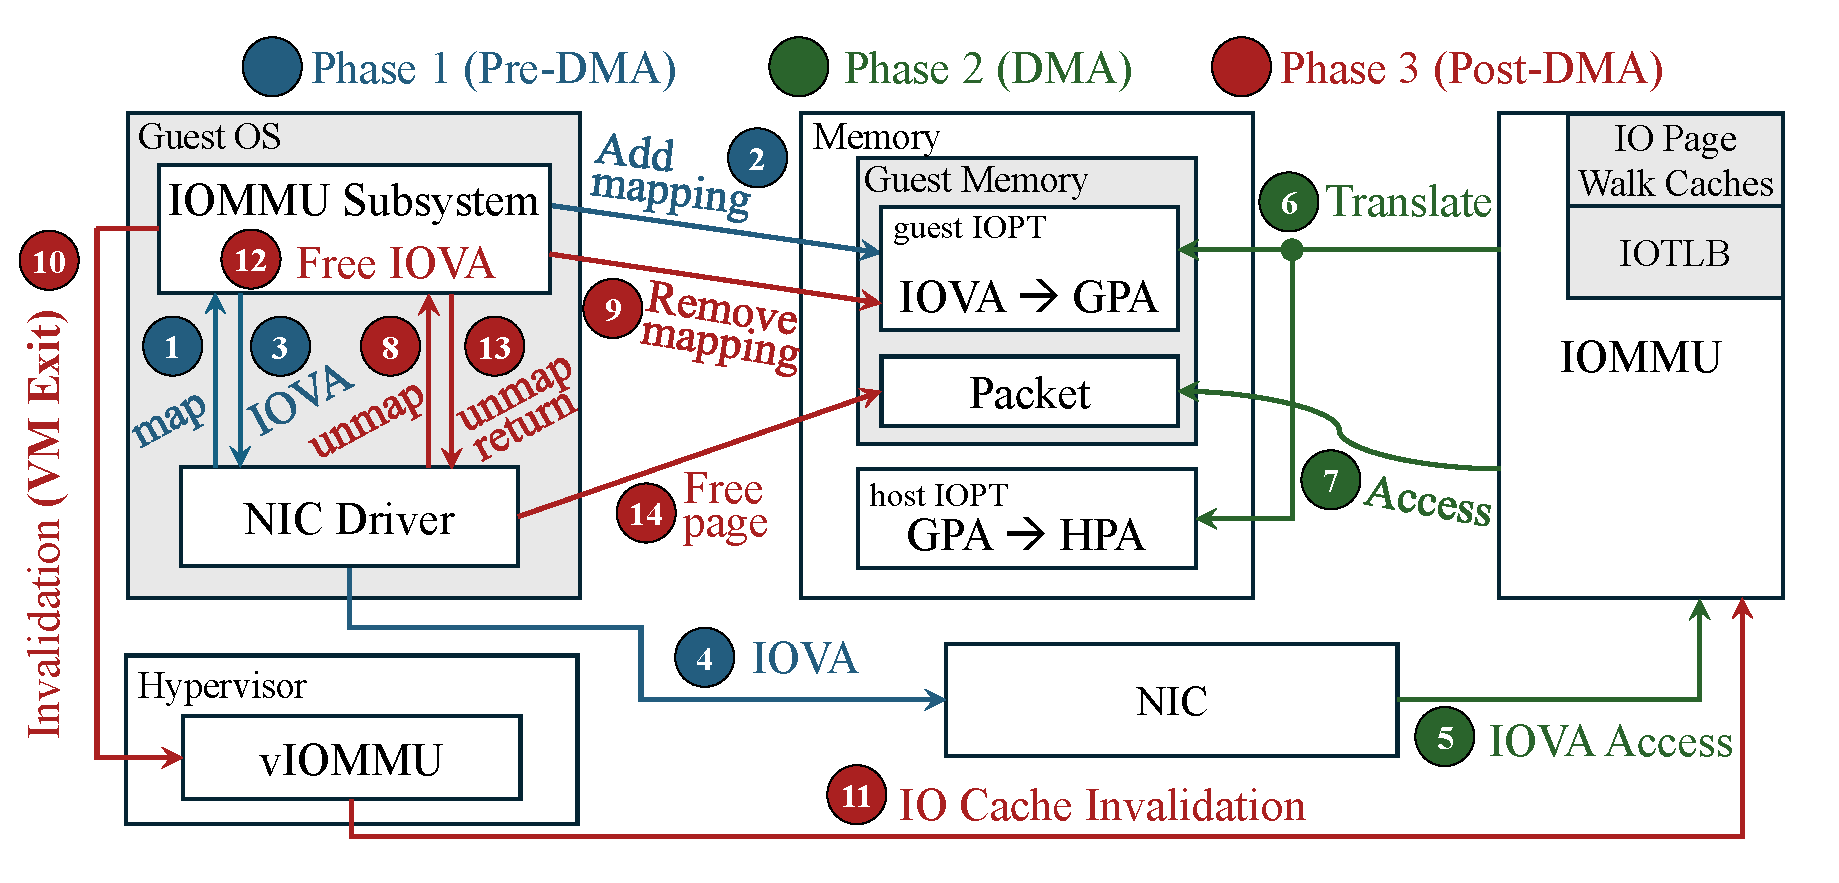
\includegraphics[width=\columnwidth]{figures/datapath_large_font_cropped.pdf}
\Description{ Illustration of NIC-to-memory DMA datapath at the transmitter when memory protection is enabled.}
\caption{\small {\bf Illustration of NIC-to-memory DMA datapath at the transmitter when memory protection is enabled.}}
\label{vfree:fig:datapath}
\end{figure}

% Bypassing the hypervisor on the I/O data path is essential to saturate modern high-speed networks bandwidth. 

% Crucially, while this passthrough mechanism applies to the NIC, it does \emph{not} extend to the host's IOMMU. 
% The IOMMU remains a shared hardware resource managed by the host, and current architectures preclude VMs from directly manipulating its hardware registers~\cite{intel_vtd_spec,qemu_10_0}.
% Consequently, the Post-DMA phase—which involve invalidating IOMMU state—still necessitates hypervisor intervention, as detailed below.
% }\saksham{I think we can get rid of this para.}

% We use Intel Emerald Rapids CPUs and Nvidia CX-7 NICs; the high-level datapath for other recent CPU architectures and NICs is similar. 

% Further, we also assume device passthrough/direct device assignment\saksham{say why?}. 

% assumptions: intel CPUs, device passthrough, linux, nested translation in IOMMU, intra-guest, viommmu in QEMU, focus on strict


\para{\BC{1} IOVA allocation and IOMMU mapping.} 
% Before the NIC is allowed to DMA the data to/from the host memory, 
The guest uses the \CodeIn{map()} API to create an IOVA-to-GPA (guest physical address) 
    mapping in the guest-local IOPT. 
The guest then creates a packet descriptor containing the IOVA, and passes 
    the descriptor to the NIC.
% \footnote{There's a slight difference in exactly when the packet descriptors (hence IOVA mappings) are created and communicated to the NIC between the NIC transmit (Tx) and receive (Rx) datapath. For Tx, descriptors are created whenever the application has some data ready to be sent to the socket, while for Rx the descriptors are pro-actively filled-up to handle future packet arrivals at the NIC. \saksham{Folks should check this footnote, and make it slightly more precise.}}. 

With device passthrough, the NIC performs data transfers without involving the host. This is possible with IOMMUs in recent Intel CPU architectures (Sapphire Rapids and newer) using 
    nested translation~\cite{intel_vtd_spec} that enables the  
    IOMMU to translate IOVAs directly to corresponding host physical addresses (HPAs) rather than GPAs,
    without host intervention.\footnote{We focus on nested translation supported by modern server hardware. 
    An alternative is to {\it shadow IOPT}, where the hypervisor 
    maintains an IOPT that maps each IOVA directly to the HPA.
    Shadow IOPT requires every new mapping to trigger a VM exit 
    for the hypervisor to update the shadow IOPT. Nested translation eliminates such VM exits.
    In our measurement, nested translation achieves strictly higher throughput than shadow IOPT,
    by 1.2$\times$ to 2.6$\times$ across core counts. 
    While we focus on nested translations, some of our techniques may also be useful for shadow IOPT.} 

\if 0
With nested translation, IOMMUs support two levels of address translations: 
    IOVA-to-GPA translation using per-guest IOPT, along with GPA-to-HPA translation 
    using a host-based IOPT. 
Typically, GPA-to-HPA updates happen infrequently (e.g., when creating a new VM), 
    and hence not on the critical path of NIC DMA operations. \rachit{why do we need this paragraph; the previous paragraph already says that nested translation enables iova-to-hpa translation}
%in this paper, we assume GPA-to-HPA mappings remain static. \leshna{I do not like this framing here, this seems like we assume the mapping to remain static only for our approach, whereas that is how it is handled in QEMU, basically a supporting statement of why this assumption is not very huge}
\fi


% To prepare a packet for transmission, the guest    invokes the DMA mapping API to map the memory page containing the packet data.
% The vIOMMU subsystem assigns an I/O virtual address (IOVA) and 
%     installs a mapping from the IOVA to the corresponding Guest Physical Address (GPA) 
%     in the guest I/O page table (IOPT);
%     the IOVA is then returned to the NIC driver.

    
% Upon DMA, the GPA is further translated by the host into a Host Physical Address (HPA).
% The host establishes the GPA-to-HPA mappings when allocating memory to the VM. 
% These mappings change infrequently and are not on the critical path of DMA operations. 
% In contrast, the guest dynamically installs IOVA-to-GPA mappings 
%     for DMA buffers. 
% When a new IOVA-to-GPA mapping is created, no host intervention or IOTLB invalidation 
%     is required because the IOVA can only be reused after the device has no stale cache translations.
   
% As a result, the mapping operation proceeds entirely within the guest without triggering a VM exit.

%        The hypervisor intercepts this invalidation,\rachit{allocates a physical page at this point?} updates the shadow page table, 
% and issues the hardware invalidation on the guest's behalf. 
% Thus, under shadow page tables, every new IOMMU mapping requires a VM exit in addition to the unmap-path VM exit. 
% We present comparative results for shadow and nested translation in \todo{fig}}

% \footnote{Under shadow page tables, the hypervisor maintains a single merged IO page table mapping IOVAs directly to HPAs.
% Because the hypervisor has no other mechanism to learn about new guest mappings, the guest must issue an IOTLB invalidation after every new mapping ---- a privileged operation that triggers a VM exit. The hypervisor intercepts this invalidation,\rachit{allocates a physical page at this point?} updates the shadow page table, and issues the hardware invalidation on the guest's behalf. Thus, under shadow page tables, every new IOMMU mapping requires a VM exit in addition to the unmap-path VM exit. We present comparative results for shadow and nested translation in \todo{fig}}

\if 0
% discussed with Leshna and this is not super relevant
\question{we have a lot of ways this is handled, do we want a description? Do I say we focus on static pinning as that will give us the best performance?, 
    On-demand page pinning (original vIOMMU paper) — hypervisor creates GPA to HPA mappings lazily, 
    invalidations; IOMMU hardware page faults (PRI/PRQ) 
    — the IOMMU itself can fault on a missing second-stage entry 
    and the hypervisor populates it on demand, 
    Dynamic scenarios like memory ballooning, live migration, etc. 
    that mutate second-stage mappings at runtime or static pinning we see in our case}
\fi

 % To initiate DMA, the guest writes the IOVA of the packet buffer 
    % into a Tx descriptor and notifies the NIC.
    % \rachit{\circled{4} should be a part of step \circled{2} in the figure?}


 \para{\BC{2} DMA and address translation.} 
The NIC issues DMA requests using the IOVA in packet descriptors,
    which triggers IOVA-to-HPA address translation using the IOMMU; 
% \leshna{this reads to me like the NIC and IOMMU are tightly coupled, like the IOMMU is part of the NIC} 
the final or intermediate translation 
    could be cached in IOMMU's IOTLB and IO PWCs~\cite{Rubin2024FastSafe}. Upon successful translation, the DMA is executed to the corresponding HPA. 
% to fetch the packet data from host memory 
    % before transmitting it over the network. 
% A single DMA operation may be split into multiple PCIe transactions 
%     depending on the request size and the maximum PCIe transaction size supported by the device and the platform.

% As these PCIe transactions reach the root complex (e.g., the Integrated I/O Controller in Intel architectures), 
%     the IOVA in each transaction must be translated into a HPA. 
% The IOMMU first consults its IOTLB. 
% On an IOTLB hit, the cached translation is used to obtain the corresponding HPA. 
% On a miss, the IOMMU performs a IOPT walk to resolve the translation, 
%     potentially involving nested translation across the guest and host IOPTs. 
% As address translation occurs at the granularity of individual PCIe transactions, 
    % multiple translations may be required to complete the DMA transfer for a single packet.
% \rachit{This paragraph should be significantly cut down; information that seem important to the rest of the paper: to initiate DMA, the guest informs the NIC of the iova; the NIC performs address translation using IOMMU; gets a physical address and transmits data at that physical address (there should be a data copy involved somewhere). requires no VM exits.}

% both stages; paging-structure caches may accelerate this walk 
%    by caching intermediate entries from either or both stages. 
\if 0
\rachit{would be nice to say how to this about nested page tables in terms of levels 
    (e.g., can L1 cache store the first level of first-stage AND the first level of second-stage?)}
\leshna{
    This in the spec explicitly mentions everything is allowed,
   the can combine or do one, based on hardware}. 
\fi

\para{\BC{3} Completion and IOMMU cache invalidation.} 
To maintain strict IO memory protection, NIC's access to the target page(s) in the host memory must be revoked immediately after the DMA completes~\cite{Rubin2024FastSafe,Amit2011vIOMMU}. This happens using two steps.
% \rachit{explicitly say: To do so, the guest invokes unmap() call which leads to removal of ....}
First, the guest uses the \CodeIn{unmap()} API which removes 
    the corresponding IOVA-to-GPA mapping from the guest IOPT.\footnote{GPA-to-HPA mapping are managed by the host. In KVM/QEMU, these mappings are established at VM creation time; for VFIO passthrough devices, guest memory is pinned, so GPA-to-HPA mappings remain static.} % and are not on the DMA critical path.} %This paper focuses on the IOVA-to-GPA mappings that 
    % change with every \CodeIn{map}/\CodeIn{unmap}.}} 
Second,
    mappings in IOMMU caches are also invalidated---typically, these invalidations are executed synchronously within the \CodeIn{unmap()} call.
The IOMMU provides an invalidation queue as an interface for the OS 
    to submit {\it invalidation requests (IRs)}. This happens in two steps (see Figure~\ref{vfree:fig:ir-ops}). 


   

\begin{enumerate}
\item {\bf Preparing the IR descriptor (IR-PREP).} 
% The first step is preparing an IR to submit to % processed by the IOMMU hardware. 
The guest kernel thread first acquires 
    a per-IO-domain 
    spinlock (termed \CodeIn{cache\_lock}~\cite{dmar_domain.cache_lock} in Linux). 
    Upon acquiring the lock, the thread prepares and enqueues 
    an IR descriptor in a per-IO-domain submission queue---referred 
    to as {\it IO-domain queue} in the guest. 
Note that there can be multiple IO-domain queues in the guest
    (\textit{e.g.}, for different devices).
%    \rachit{this may confuse the reader: if the thread keeps both cache-lock and q-lock, why does it need to copy the request to the SW queue; why can't it directly write to the emulated invalidation queue?}

% \rachit{IIRC, we never define a device, and never say that devices share IO virtual address spaces; we should define devices and say it in S2}. \rachit{is it true that only the vCPUs within a single VM contend on this lock? are vCPUs in different VMs in different domains in vIOMMU?}
% As an IOMMU domain may have multiple physical devices, the kernel needs to ensure the IOMMU caches for each of the devices are flushed. 
% While holding this lock, the thread iterates over the domain's list of \emph{cache tags}---metadata 
%     entries that record which hardware caches may hold translations for IO devices in this domain (e.g., IOTLB in IOMMU or ATS-supported NICs~\cite{}\saksham{need references}). 
% For each cache tag, the kernel prepares the appropriate IR, specifying the IOVA range to invalidate. 
% % and whether to flush IOTLB entries alone or additionally flush page-table cache entries. The descriptors are accumulated into a batch for the physical IOMMU hardware unit of the device. 
% % \rachit{the text is very clear now, great. However, I (and hence, may be other readers) wonder: why does the kernel need to ensure that IOMMU caches for all devices are flushed? [Update] Ha, I see it is answered in the next paragraph.}.
% The lock ensures safe access of the cache tags for IR-PREP,
%     preventing data races caused by concurrent updates 
%     of the cache-tag list (e.g., a concurrent 
%     detach of an I/O device would free its cache-tag list).
% % Specifically, if a device were detached while iterating over the list, the cache tag entry could be freed underneath the iterator, resulting in a use-after-free.  
% % Conversely, if a device were attached mid-flush, the new device's caches might not receive the invalidation, leaving stale translations that violate the strict guarantee.  \CodeIn{cache\_lock} serializes flushes against structural
% % modifications to prevent both hazards.
% % \rachit{use-after-free discussion makes sense but this is a cache, so use-after-free should not lead to any errors---right?}
% % For the device attachment, why would a newly attached device have cache entries?}
% However, this lock serializes IR-PREP operations 
%     for all threads in the same IO domain in the VM.
% Upon acquiring the lock and preparing the IR, it is enqueued in a (per-IO-domain) submission queue---referred 
%     to as SW queue within the guest kernel\saksham{check if true}.

\item {\bf Submitting the IR to IOMMU hardware (IR-SUB):} 
% \para{\circledx{2} Hardware queue submission under \CodeIn{q\_lock}.} 
To submit the IR descriptors in an IO-domain 
    queue to the IOMMU hardware, 
    the hypervisor, specifically the vIOMMU subsystem, exposes 
    an {\it emulated IOMMU invalidation queue} to the guest.
% This is the interface available to each guest to submit IRs to the IOMMU hardware. 
Before submitting the IR to the emulated invalidation queue, the guest needs to acquire another lock---a 
    per-invalidation-queue spinlock (\CodeIn{q\_lock}{~\cite{q_inval.q_lock}} in Linux). 
% This serializes access to the emulated invalidation queue for IRs from all threads within the guest; 
% otherwise, concurrent writers could corrupt the queue by overwriting each other's IRs. 
    While holding \CodeIn{q\_lock}, the kernel writes the IR descriptor into the queue, 
    then advances a tail register---via an MMIO write---to signal the hardware 
    to process the IR. 
% \rachit{guest/kernel inconsistency; also the text says that the ``the'' guest thread: is it different from the network thread above?}
\end{enumerate}






 % While holding \texttt{q\_lock}, the kernel writes the batch of invalidation descriptors and a trailing wait descriptor into the queue, then advances the tail register via an MMIO write.

    % \para{\circledx{3} VM~exit and busy-wait.} 
    %  The MMIO write to the tail register triggers an \texttt{EPT\_MISCONFIG} VM~exit, transferring control to the hypervisor.  The hypervisor validates the invalidation request, issues the corresponding hardware invalidation on the physical IOMMU, and returns control to the guest.  The guest CPU then busy-waits on the status field written by the wait descriptor until the hardware signals that the invalidation is complete.  Only then are both locks released and the physical page made available for recycling.
\noindent
{\bf Unavoidable VM exit for {\em every} IR.} 
Submitting IRs from the guest to the IOMMU hardware necessarily requires hypervisor intervention. 
This is because the IOMMU invalidation queue---the interface provided to the OS for IOMMU cache invalidation---is 
    a shared host resource with no per-VM partitioning~\cite{intel_vtd_spec_caching}; 
    allowing multiple guests to write concurrently would risk corruption. Thus, the MMIO write to the tail register
% Every IR-SUB operation to the emulated invalidation queue 
triggers a 
% \CodeIn{EPT\_MISCONFIG} 
VM~exit, transferring control to the hypervisor.  The hypervisor validates the IR, issues the corresponding IR to the physical IOMMU (by copying the IR to the IOMMU invalidation queue in the host), and returns control to the guest.  The guest thread, in the meantime, busy-waits on the status field until the hardware signals that the invalidation is complete.  
% Consequently, the guest must trap into the host, incuring an unavoidable VM exit~\cite{qemu_intel_iommu_c} during unmaps.
% Only then are both locks released.
So, the VM exit is performed for {\em every} IR,
because an IR descriptor is written to the emulated queue protected
    by \CodeIn{cache\_lock} (\CodeIn{q\_lock} 
    is acquired \emph{inside} \CodeIn{cache\_lock}). 
% The nesting of the two critical sections is not a major performance bottleneck
    % on bare mental (taking less than one microsecond).
% However, it becomes significantly more expensive in virtualized environment (see \S\ref{vfree:sec:pointer}).
% This is likely done to avoid re-acquiring the \CodeIn{cache\_lock} 
%    to copy the IR from the SW queue to emulated invalidation queue \rachit{I understand we are doing it in our final design (as we discussed)? if so, we should avoid this sentence otherwise we need to outline our key insight on why we can do it.}. 
% Therefore, each IR triggers an independent VM exit. 

 





% Each physical IOMMU has its own invalidation queue



 % and its own \CodeIn{q\_lock}; 

    
% This queue is shared across all cores; 
% While holding \CodeIn{q\_lock}, the kernel writes the batch of invalidation descriptors and a trailing wait descriptor into the queue, then advances the tail register via an MMIO write.





% \rachit{a bit of restructuring the rest of this paragraph will be helpful: while the guest can remove iova-to-gpa mappings, mappings in IOTLB and IOPT caches must also be invalidated---this requires hypervisor intervention; then move the next two sentences to after describing why the intervention is needed.}

\begin{figure}[H]
	\centering
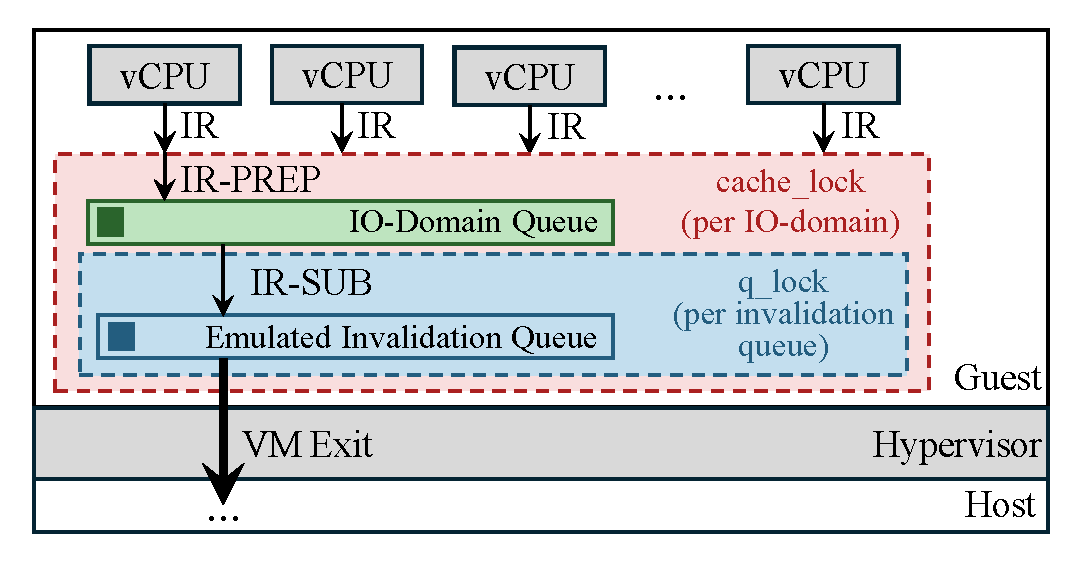
\includegraphics[width=0.72\columnwidth]
{figures/background_guest_queues_cropped.pdf}
\caption{\small {\bf IR-PREP and IR-SUB operations in the Post-DMA phase and the corresponding queues.}}
\label{vfree:fig:ir-ops}
\end{figure}

% The vIOMMU then invalidates the affected entries in all IOMMU caches, including the IOTLB and IOPT caches, 
    
    
% \saksham{Need to describe the invalidation process in more details here, the cache lock, shared SW Q, q lock, emulated HW q, hypervisor trap, and corresponding host operations.} \saksham{Also talk about strict safety guarantee here, about synchronously invalidating after unmaps.}


% Unlike mapping new pages, unmapping \emph{always} 

% , which serializes invalidation requests 
%     and issues the hardware invalidation on the guest's behalf. 
    
 % \para{\circledx{3} VM~exit and busy-wait.} 

\noindent
Finally, upon successful IR processing, the IOVA is returned to the IOVA allocator and the corresponding physical page(s) 
    used for DMA are made available for recycling. 
Both \CodeIn{cache\_lock} and \CodeIn{q\_lock} are released when IR-SUB finishes.
% \rachit{say when the locks are released}

% \vspace{0.1in}
% \paragraphb{Strict memory protection} Linux today enforces strict memory protection by performing IR processing synchronously with {\tt unmap()} call. 

% \paragraph{Tx Datapath}
% \label{vfree:sec:tx-datapath}
% Every transmitted network packet---including TCP \leshnaedit{acknowledgements} generated in response to received data---goes
%     through a per-packet IOMMU lifecycle in the follows steps:
% %\begin{enumerate}[leftmargin=*,label=\protect\circledb{\arabic*}]
% % \item 
% \paragraph{\bf Rx Datapath.}
% \label{vfree:sec:rx-datapath}
% The Rx datapath follows the IOMMU mapping, address translation, and invalidation steps (\BC{1}--\BC{3}) as the Tx datapath steps, 
%     but does so in the reverse direction: the NIC DMAs incoming packet data 
%     into host memory rather than reading it out. 

\para{Optimizations for Rx Datapath in Linux.}
% \label{vfree:sec:linux-opt}
Recent versions of Linux network stack (>=6.11~\cite{linux_page_pool_netmem}) implement
    an optimization in the Rx datapath to reduce \CodeIn{map()}
    and \CodeIn{unmap()} operations.{\footnote{For several pragmatic reasons, existing operating systems do not apply similar optimizations on the Tx datapath.
% , 
%     because typically no data-copy operation is involved between the kernel and userspace buffers: 
%     NIC directly DMA's data from the userspace \rachit{are we sure?} buffers in the Tx datapath, 
%     and the NIC can maliciously access the DMA buffers if permanently mapped IOVAs are used. 
%
Hence, every transmitted packet incurs at least one VM exit per \CodeIn{unmap()} call.}}
It uses a per-CPU cache to maintain a set of IOVAs permanently mapped to the IOMMU~\cite{markuze2018damn}. 
In the Rx datapath, the kernel uses the physical pages mapped to these IOVAs to allocated kernel-space buffers 
    (\textit{e.g.}, TCP socket buffers), used to DMA data from the NIC. 
Upon DMA, the data is copied from kernel-space buffers to the userspace buffers, 
    before returning back the IOVA to the cache.
Malicious NIC with access to the IOVA cannot access the userspace buffers (which are not mapped to the IOMMU). 
Using (and recycling) these IOVAs therefore do not require \CodeIn{map()}/\CodeIn{unmap()} calls. 
This optimization is helpful for workloads for which actively used IOVAs are consistently smaller than the cache size~\cite{Rubin2024FastSafe}. 
Upon exhausting this cache, whenever the kernel requires another IOVA, 
it uses the default IOVA allocation/deallocation datapath, 
using regular \CodeIn{map()}/\CodeIn{unmap()} operations.
%  as discussed previously in this section.
% The page pool consists of a small per-CPU cache (64~entries in mlx5 \tianyin{??}) backed by a larger pointer ring (1024~entries) \rachit{is it important to distinguish between the two? if not, that seems unnecessary detail}. 
% Every page in the pool carries a valid IOVA mapping, established when the page first enters the pool and persists as long as the page remains in it. 
% On the receive fast path, the driver retrieves a pre-mapped page from the cache, installs its IOVA into an Rx descriptor, and marks it ready to receive---no IOMMU interaction is needed. Upon completion of DMA, the page is returned to the page pool. If the pool has space (the cache or pointer ring is not full), the page is placed back with its IOVA mapping unchanged. No IOMMU operation occurs and no VM~exit is triggered. 



% {Why it works for Rx side only?}
% This is feasible because on the receive side, the driver owns the page from allocation through free and can keep it persistently mapped without friction. 
% On the transmit side, no such pool exists because the kernel does not often own the page being sent. the payload resides in userspace memory; thus, the driver cannot recycle the userspace pages in a pre-mapped pool without performing expensive data copies. 


% An important difference is that modern NIC drivers maintain a per-CPU \emph{page pool} that eliminates most IOMMU operations from the Rx fast path. 

% \leshnaedit{In our setup \S\ref{vfree:sec:inefficiencies}, over 99.9\% IOMMU operations on the Rx data path are skipped by page pool.}








\subsection{Understanding Protection Overhead}
\label{vfree:sec:inefficiencies}
This section builds an in-depth understanding of inefficiencies in existing strict intra-VM IO memory protection mechanisms. We present more results, including those for real-world applications 
  in \S\ref{vfree:sec:eval}.
%We also provide insights into the fundamental reasons behind the observed degradation. 
% Our key findings are:
% \begin{itemize}[leftmargin=*]
% \item State-of-the-art IO memory protection mechanisms introduce significant performance degradation---reducing 
%   the peak throughput by as much as {$\sim$}60-95\% compared to the no protection case. 
%   Using additional cores to run networked applications does not improve throughput; 
%   in fact, we observe a surprising phenomenon: beyond a certain point, assigning more cores to the application can actually result in lower than the peak throughput. 
% % throughput reaches only 145\,Gbps at 12~cores and then \emph{decreases} with additional cores---dropping by 3$\times$ at 24~cores---exhibiting anti-scaling behavior.

% \item The {\it root cause} of low peak throughput is that today each invalidation request (IR)
% %  is serialized across all threads in the VM, 
%   necessitates {\it at least one VM exit}. 
%   This limits the maximum aggregate rate of IRs, 
%   and thus the maximum achievable network throughput, independent of the number of cores running the application. 

% % is not the cost of any single VM~exit, but the \emph{serialization} of all cores' invalidations through a single hardware resource whose access requires a VM~exit.  This serialization caps the system's aggregate invalidation throughput independent of core count.
% \item The {\it root cause} for the surprising phenomenon is more subtle. Virtualization introduces an intricate feedback loop between lock contention 
%   and hypervisor scheduling: 
%   when vCPUs contend for invalidation, those that fail to aquire the lock are descheduled by the hypervisor. 
% Waking these vCPUs requires hypercalls and inter-processor interrupts (IPIs) that further trigger 
%   VM~exits, inflating lock acquisition time and causing 
%   even more vCPUs to be descheduled. 
%   Such a feedback loop causes performance to degrade beyond VM-exit overhead
%   %  beyond the serialization-imposed throughput limit
%   as the number of cores increase.
% \end{itemize}

\para{Measurement Setup.}
% \schaic{All comments resolved. @Rachit please check.}
We use two servers directly connected to each other via $400$Gbps Nvidia ConnectX-7 NICs to ensure performance bottlenecks not in the 
  network. 
The servers use Emerald Rapids processor architecture that supports nested translation,
  with Intel Xeon Platinum 8592V CPUs and Intel Xeon Gold 6538Y+ CPUs respectively. 
The former hosts our VMs, 
  and the latter acts as client to send or receive traffic to the VM. 
  % a passive server engaged in Rx or Tx traffic 
  % \rachit{we have to be careful: each server does both Rx and Tx---right?}.  
% Each server has an Nvidia ConnectX-7 NIC; the two NICs connected to Ethernet with 400Gbps access link bandwidth.
% The host server is a 4-socket server; each socket has
%   32 physical cores, 252GB of memory and 150GB/s of memory bandwidth.
  % per-socket. 
The host server, guest VM, and client machines run with Ubuntu 22.04 and Linux v6.12.9. 
% \saksham{KVM/QEMU versions?} 
The VMs are hosted by QEMU v10.0 with nested translation~\cite{yiliu1765qemu}.
% \saksham{Static pinning of vCPUs to physical cores to avoid interference.} 
We place the VMs on the NIC-local NUMA node.
Every vCPU of the VM is pinned to a separate physical core on the host to avoid interference. See \S\ref{vfree:sec:eval} for more details.
  % We disable hyperthreading, CPU frequency scaling (we fix cores at their base frequency), and NUMA balancing for stable performance. 
% We built a ebpf-based tool to measure the performance of guest and host OS.
% \saksham{if we get time, we should add error bars with stddev}.
% \schaic{We already have errors bars in the latest version @Saksham.}

We use Iperf3~\cite{iperf3} to generate network traffic with $4$K MTU size, and measure throughput.
% We measure CPU utilization with sar~\cite{sar}.
% We use eBPF probes to record the execution time and invocation counts of relevant kernel functions.
% We measure VM exit counts, reasons, and time with perf~\cite{perf}.
% We enabled TCP Segmentation Offload (TSO), Generic Receive Offload (GRO), and adaptive Receive Flow Steering (aRFS) 
% to reflect high-performance networks. 
We run each experiment five times, and present the average results and standard deviation. We use two setups to isolate the impact of IO memory protection on Rx and Tx datapaths. In the {\bf Rx-server} setup, the client sends large payloads to the VM; the VM receives these payloads and transmits TCP ACKs back to the client. In the {\bf Tx-server} setup, the VM sends large payloads to the client and receives TCP ACKs from the client.




% We run the VM as receiver (Rx) 
%   and trasmitter (Tx) 
%   of network traffic, respectively, in two sets of experiments; this helps us isolate the impact of I/O memory protection on each setup. \rachit{this continues to be very confusing---saying that VM is the receiver of network traffic is incorrect since it also does Tx. We should precisely define what these two setups are: Rx receives large payloads and transmits ACKs; Tx transmits large payloads and receives ACKs;}
% Tx and Rx cases separately to isolate the impact of I/O memory protection on each datapath
%   (full-system results in \S\ref{vfree:sec:eval}). 
  % \rachit{readers may find this confusing---each server does both Rx and Tx.}
% later in eval section we run an end-to-end scenario where both kinds of traffic are running concurrently.
% \schai{: receive (Figure~\ref{vfree:fig:motivation-rx}) and transmit (Figure~\ref{vfree:fig:motivation-tx}).
% \noindent
% We increase the number of flows (each pinned to a core in the VM)
%   and compare throughput when running with
%   (1) vIOMMU off and (2) vIOMMU with strict memory protection (using nested translation).
% This section presents minimalist results to build an in-depth understanding of inefficiencies in strict intra-guest IO memory protection;  
  

% \begin{figure}
% 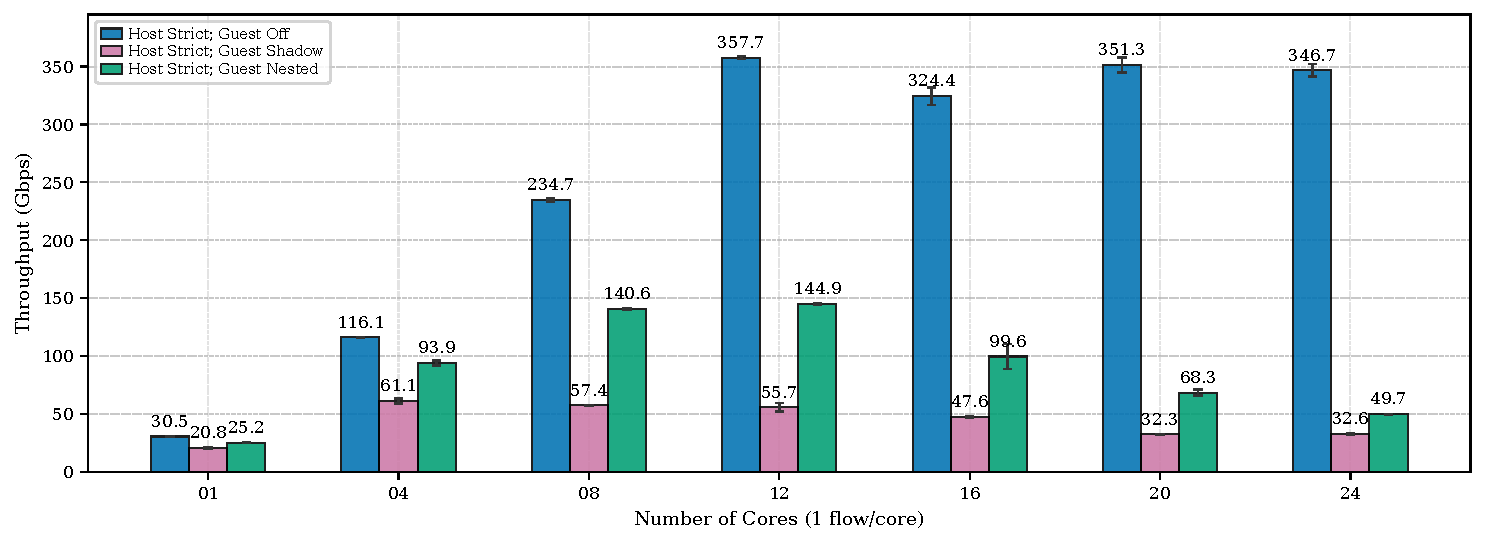
\includegraphics[width=\columnwidth]{figures/baseline-iperf-tput.pdf}
% \Description{Throughput vs Number of Cores Viommu off, Shadow and Nested}
% \caption{Throughput vs Number of Cores Viommu off, Shadow and Nested \saksham{I think we should get rid of shadow results?}}
% \label{vfree:fig:baseline-iperf}
% \end{figure}

\begin{figure}[H]
    \centering
    \begin{subfigure}[b]{\columnwidth}
        \centering
        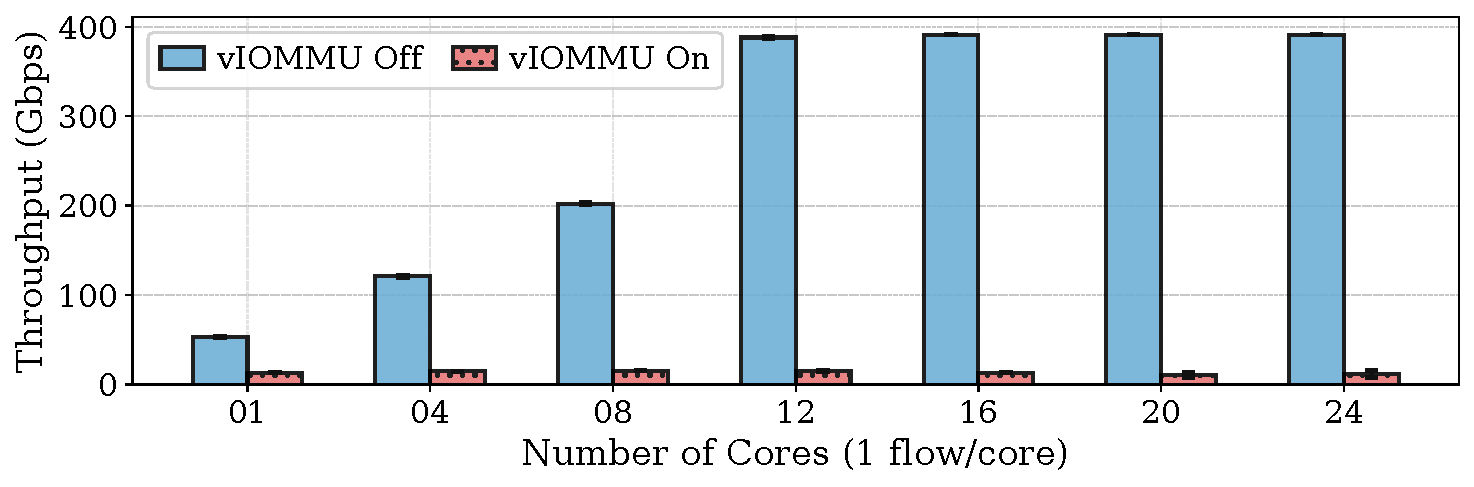
\includegraphics[width=\textwidth]{figures/motivation_tx_varying_cores-tput.pdf}
        \caption{Tx-server (VM running as a transmitter)}
        \label{vfree:fig:motivation-tx}
    \end{subfigure}
    \begin{subfigure}[b]{\columnwidth}
        \centering
        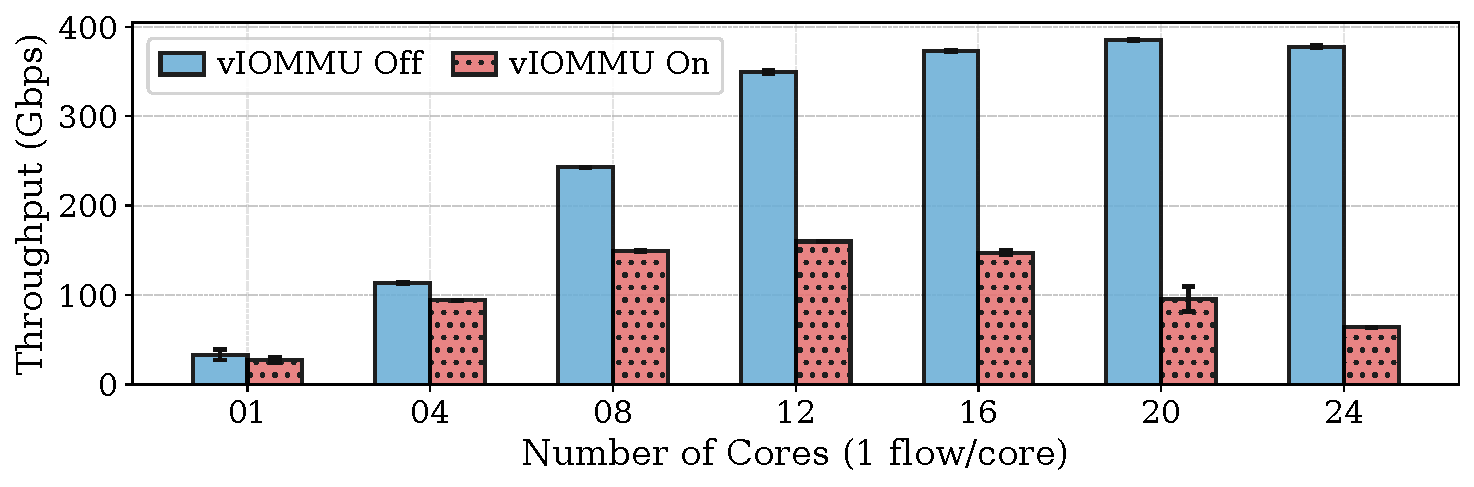
\includegraphics[width=\textwidth]{figures/motivation_rx-tput.pdf}
        % \caption{Rx throughput}
        \caption{Rx-server (VM running as a receiver)}
        \label{vfree:fig:motivation-rx}
    \end{subfigure}
    \caption{\small {\bf State-of-the-art IO memory protection mechanisms suffer from significant performance degradation compared to the unprotected mode,
    and exhibit anti-scaling behavior with increasing cores.} Performance degradation is much more profound on the Tx-server setup.}
    \label{vfree:fig:baseline-iperf}
\end{figure}


\paragraphb{[Figure~\ref{vfree:fig:baseline-iperf}] Performance degradation with IO memory protection in VMs}
% Figure~\ref{vfree:fig:motivation} compares network throughput with increasing number of cores\saksham{should we use vCPUs, or cores in our discussion?} for three configurations: (1) vIOMMU disabled, (2) \sout{vIOMMU strict mode with shadow page tables,} and (3) vIOMMU enabled with strict memory protection and nested translation.
% Figure~\ref{vfree:fig:motivation-rx} and \ref{vfree:fig:motivation-tx} compare network throughput with increasing number of flows (each flow pinned to a core in the VM)
%   for two configurations: (1) vIOMMU disabled and (2) vIOMMU enabled with strict memory protection and nested translation.
Figure~\ref{vfree:fig:motivation-tx} shows throughput for the Tx-server.
Without IO memory protection, $12$ cores are sufficient to saturate the network bandwidth; thus, the achievable throughput increases until $12$ cores and plateaus thereafter.
With IO memory protection enabled, the maximum achievable throughput, 
  irrespective of number of cores used, 
  is ${\sim}$15\,Gbps---a ${\sim}$95+\% degradation 
  compared to no protection.

Figure~\ref{vfree:fig:motivation-rx} shows throughput for the Rx-server.
% With vIOMMU off, the throughput can be as high as ${\sim} 385$Gbps.
%; 12~cores is the minimum to saturate the link, 
 % where Rx throughput reaches 350Gbps .
% \rachit{is 357 the best achievable for a 400gbps link? whats the pcie bandwidth?}
% \sout{Enabling strict mode with shadow page tables---where \emph{both} map and unmap operations require VM~exits---reduces 
  % throughput to 55\,Gbps at 12~cores. }
% \sout{Switching to nested translation, which eliminates VM~exits on the map path, 
%   improves throughput to 145\,Gbps at 12~cores.  
% While nested translation recovers 90\,Gbps compared to shadow mode, 
%   a 60\% gap relative to the unprotected baseline remains.} 
Enabling IO memory protection again results in significant degradation in throughput: we observe a peak throughput of $160$Gbps with $12$ cores---{$\sim$}54\% degradation compared to the no protection case. 
Upon increasing the number of cores beyond 12, the throughput, rather surprisingly, 
  starts to drop; we observed a maximum degradation of up to $\sim$83\% when using 24 cores. 
Compared with the Tx-server case, the relatively higher Rx-server throughput is due to the page pool optimization that reduces map/unmap operations (\S\ref{vfree:sec:background-datapath}); and TCP ACK coalescing, which increases the number of pages 
  per \CodeIn{unmap} (by as much as ${\sim}15\times$).


\if 0
\schai{
We also compare the throughput under the same setup between vIOMMU running on traditional shadow page tables 
  and on nested translation.
We find that the nested translation configuration achieves strictly higher throughput than shadow page tables,
  by 1.2$\times$ to 2.6$\times$ across core counts (\textit{e.g.}, 144.9 vs.\ 55.7\,Gbps at 12~cores).
The difference comes from the fact that with shadow page tables, both map and unmap operations require VM~exits, 
  while with nested translation, only unmap operations require VM~exits.}
\fi

\paragraphb{[Figure~\ref{vfree:fig:lock-contention}] Root cause of performance degradation with IO memory protection: 
  at least one VM exit per unmap/invalidation}
IO memory protection introduces two extra operations on the datapath: \CodeIn{map()} and \CodeIn{unmap()}. 
With nested translation,
\CodeIn{unmap} is far more costly than \CodeIn{map}: 
  besides updating IOPTs, \CodeIn{unmap} also performs IOMMU cache invalidations which 
  require VM exits (\S\ref{vfree:sec:background-datapath}).
We observe that overheads of unmap operations
  are the primary contributor to the performance degradation due to IO memory protection.
  % \footnote{In vanilla Linux,
  %   the overhead of \texttt{\footnotesize unmap} further slows down \CodeIn{map}
  %   as the \texttt{\footnotesize map} implementation tries to acquire 
  %   the \texttt{\footnotesize cache\_lock} for IR processing which is only needed for shadow IOPT, not nested 
  %   translation. Unfortunately, the check is done inside \texttt{\footnotesize cache\_lock}.
  %   We optimized the behavior in \S\ref{vfree:sec:impl}. \rachit{I suggest removing this footnote}}
  % % of the above t degradation 
  % compared to vIOMMU off.

% Our kernel profiling shows that the average \CodeIn{unmap} latency 
%  is orders of magnitude higher than \CodeIn{map}'s\saksham{Verify this} 
% \rachit{precision will be helpful here---present exact numbers}. 
% So, we focus on the \CodeIn{unmap} to understand the root causes of observed performance trends. 

We observe that processing IRs within the \CodeIn{unmap} operation accounts for over {$95\%$} of the total \CodeIn{unmap()} latency on average, across all vCPU counts in both the Rx-server and the Tx-server setup (not shown; measured via eBPF probes on the unmap path). Thus, we dug deeper into IR processing overheads.
%
% \leshna{alternate text for the above: Invalidation request~(IR) processing within the \CodeIn{unmap} 
%   operation accounts for over {$95\%$} of the total \CodeIn{unmap} 
%   latency on average, across all vCPU counts in both the Rx 
%   and Tx setups (measured via eBPF probes on the unmap path).}
%
Figure~\ref{vfree:fig:lock-contention} shows the average IR processing latency per \CodeIn{unmap}
  and its breakdown across different operations involved in IR-SUB datapath (\S\ref{vfree:sec:background-datapath}). 
We observe that, as the number of cores increases, IR processing latencies increase. This increase in IR processing latency is rooted in two key characteristics of the existing IR processing path (phase \BC{3} in \S\ref{vfree:sec:background-datapath}): 
(1) the vCPU performing IR-PREP must acquire a per-IO-domain \CodeIn{cache\_lock} {\it before} preparing the IR; and 
% \leshna{each thread needs lock not vCPU hence the term here}
(2)  IR-SUB is executed {\it inside} the critical section of the same \CodeIn{cache\_lock}.
Since IR-PREP and IR-SUB are tightly coupled under one lock, 
  every invalidation request triggers its own VM exit
  (Figure~\ref{vfree:fig:current-design}).
As a result, all concurrent vCPUs serialize on 
  \CodeIn{cache\_lock} for every \CodeIn{unmap}. 

\begin{figure}[H]
	\centering
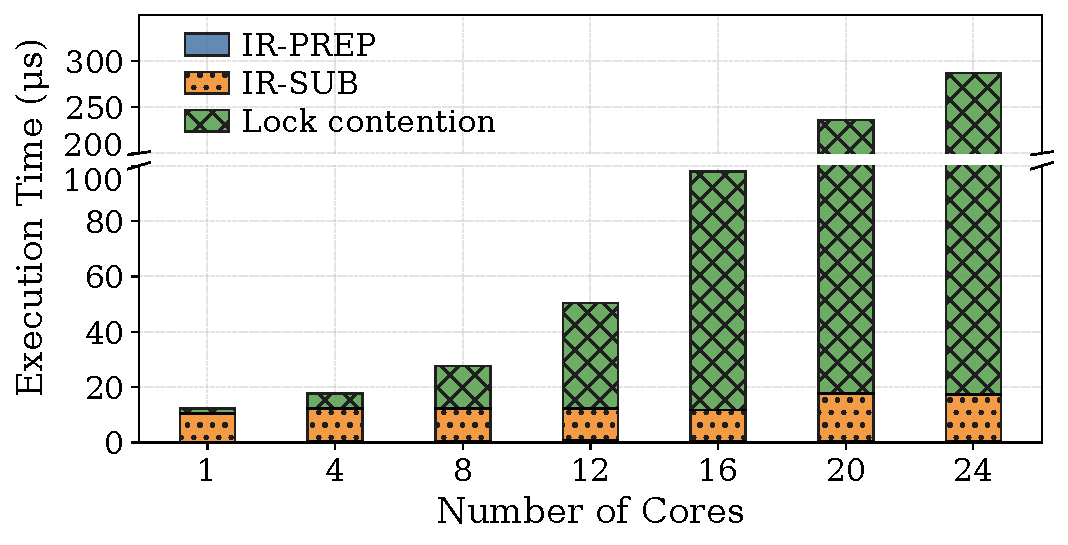
\includegraphics[width=0.7\columnwidth]{figures/siyuan_invalidation_breakdown.pdf}
% \Description{Lock Contention Time Balloons with increasing core count}
\caption{\small {\bf Breakdown of IO memory protection overheads.} IR-PREP contributes minimally, independent of number of cores. For fewer than $8$ cores, IR-SUB cost dominates; for $8$ and more cores, lock contention overheads dominate. Moreover, with increasing number of cores, lock contention time increases superlinearly while the IR-SUB cost remains nearly constant.
}
% \saksham{Linear plot with broken y-axis here.}}
\label{vfree:fig:lock-contention}
\end{figure}

Figure~\ref{vfree:fig:lock-contention} shows the consequence: 
  as the number of vCPUs increases, the time spent waiting 
  to acquire \CodeIn{cache\_lock} grows, 
  while the time for IR-PREP and IR-SUB themselves remains 
  nearly constant. In other words, the actual work per invalidation grows only modestly with scale---the dominant increase is wasted time 
  spent serializing behind other vCPUs.
Each vCPU blocks on its \CodeIn{unmap} call for the duration 
  of this wait, so per-vCPU throughput drops as contention 
  increases.

\if 0
The serialization limits the maximum rate at which the guest can perform \CodeIn{unmap} 
  per unit time (denoted as $R$), independent of the number of concurrent cores performing them: 
  $R < 1/L$ where $L$ is the time to execute the critical section of \CodeIn{cache\_lock}, \textit{i.e.}, the time 
    to execute both IR-PREP and IR-SUB operations. 
The serialization also limits the number of unmap operations 
  needed per unit of transferred network data: if we require an unmap for every $k$ pages transferred on average, 
  the achieved throughput $T < k \times 4KB / L$. For example, for the Tx-host case, 
  we measured $k = 5.5$ ($k>1$ because \CodeIn{map()}/\CodeIn{unmap()} can be performed on 
  a batch of packets in Linux~\cite{Rubin2024FastSafe}). 
  We also measured {$L = 10{\mu}s$}, giving us $T = {\sim}18$Gbps; 
  the observed Tx-host saturation throughput (${\sim}15$Gbps) is within this bound. \rachit{this paragraph is stating the obvious (throughput inversely proportional to lock contention time), brings up unnecessary issues (we never talked about batching in datapath) and is distracting; I suggest removing it.}

% The Serialization especially hurts the performance above because of the large value of $L$. 
Importantly, a majority time out of $L$ (>90\%) is spent on the {\it unavoidable VM exit} 
  required to submit the IR to the IOMMU invalidation queue in the host (see \S\ref{vfree:sec:sec:background-datapath}); 
VM exits typically incur several ${\mu}s$ worth overhead~\cite{vmexit1,vmexit2}. 
While this may have been acceptable with lower I/O speeds in the past, 
  it leads to significantly under-utilized IO bandwidth with 
  current trends of rapidly increasing IO bandwidths. \rachit{if the paper story is about VM exits, this discussion is getting too little real estate.} \rachit{this will benefit significantly from showing the number of VM exits}
\fi 

%  and stagnant VM exit overheads 
%  are leading to larger IO bandwidth underutilized.


% our evaluated workload is a best-case scenario for the optimization, 
%   where the IOVA working set size remains low and thus 
%   most IOVAs used to receive payloads do not require map/unmap operations. 
% However, Rx still needs to perform map/unmap operations for transmitted packets, 
%   such as TCP ACK packets back to the sender. 
% Due to TCP sending aggregated ACKs for multiple packets, the amount of pages transfered per \CodeIn{unmap} (i.e., $k$) 
%   is higher in the Rx case compared to Tx. 
% We measured $k$ to be ${\sim}15\times$ higher, and correspondingly the maximum achievable throughput (${\sim}215$Gbps), 
%   which is still significantly lower than the I/O bandwidth (400Gbps). 
% The maximum measured throughput (145Gbps) lies well within this bound. \rachit{this paragraph could be reduced to 1 line: rx has higher throughput due to optimizations discussed in 2.2 (give them some name) and due to ACK coelescing on the Rx side; note that this is not too important.}

\if 0
\begin{figure}[H]
	\centering
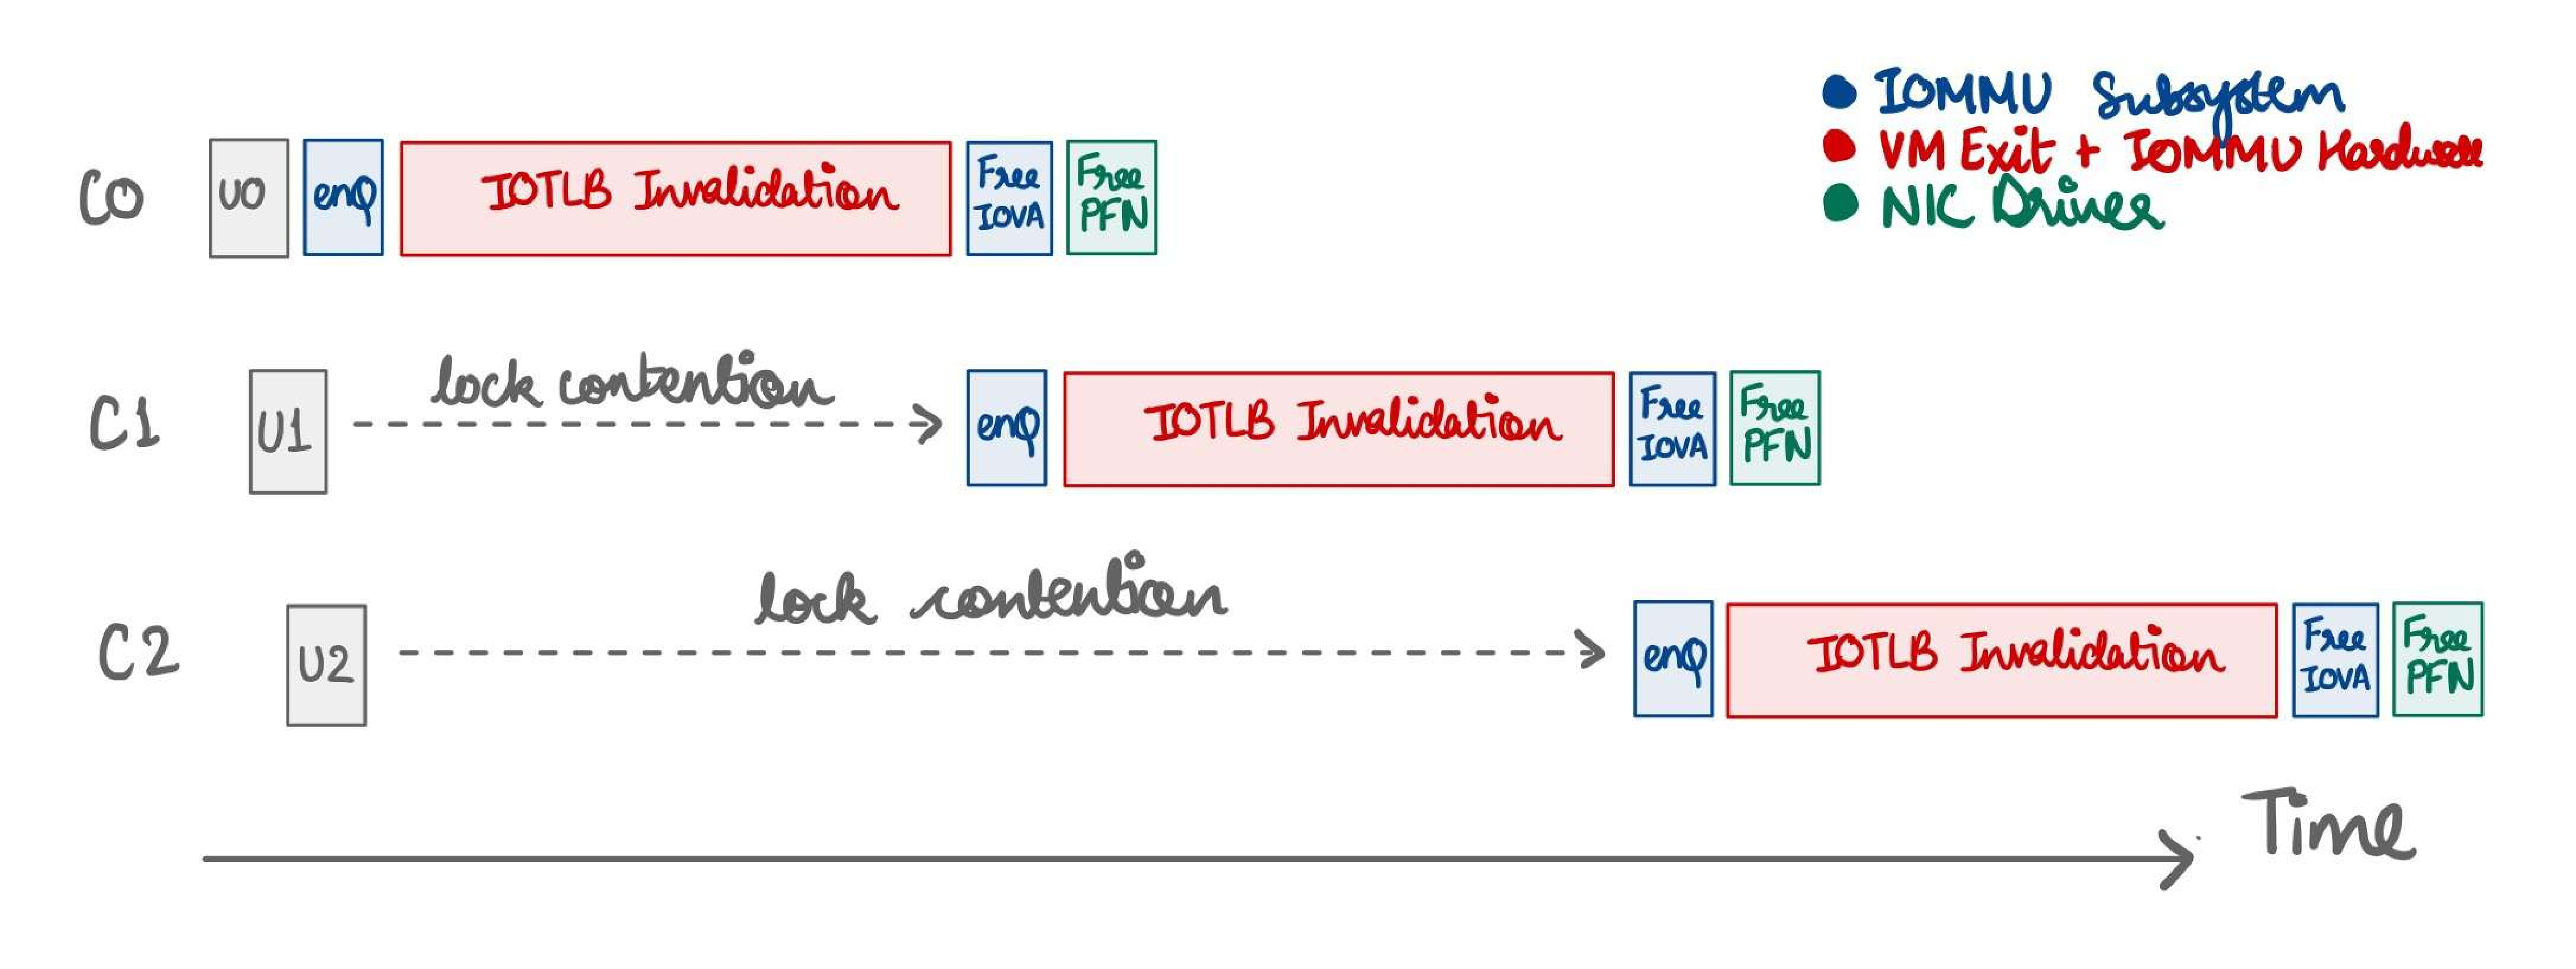
\includegraphics[width=\columnwidth]{figures/hd-default-serialization.pdf}
\Description{Serialization in current strict}
\caption{\saksham{Add pipeline bubbles here because of thread wakeups, leading to lower throughput}}
\label{vfree:fig:current-design-hlt}
\end{figure}
\fi 

\begin{figure}[H]
	\centering
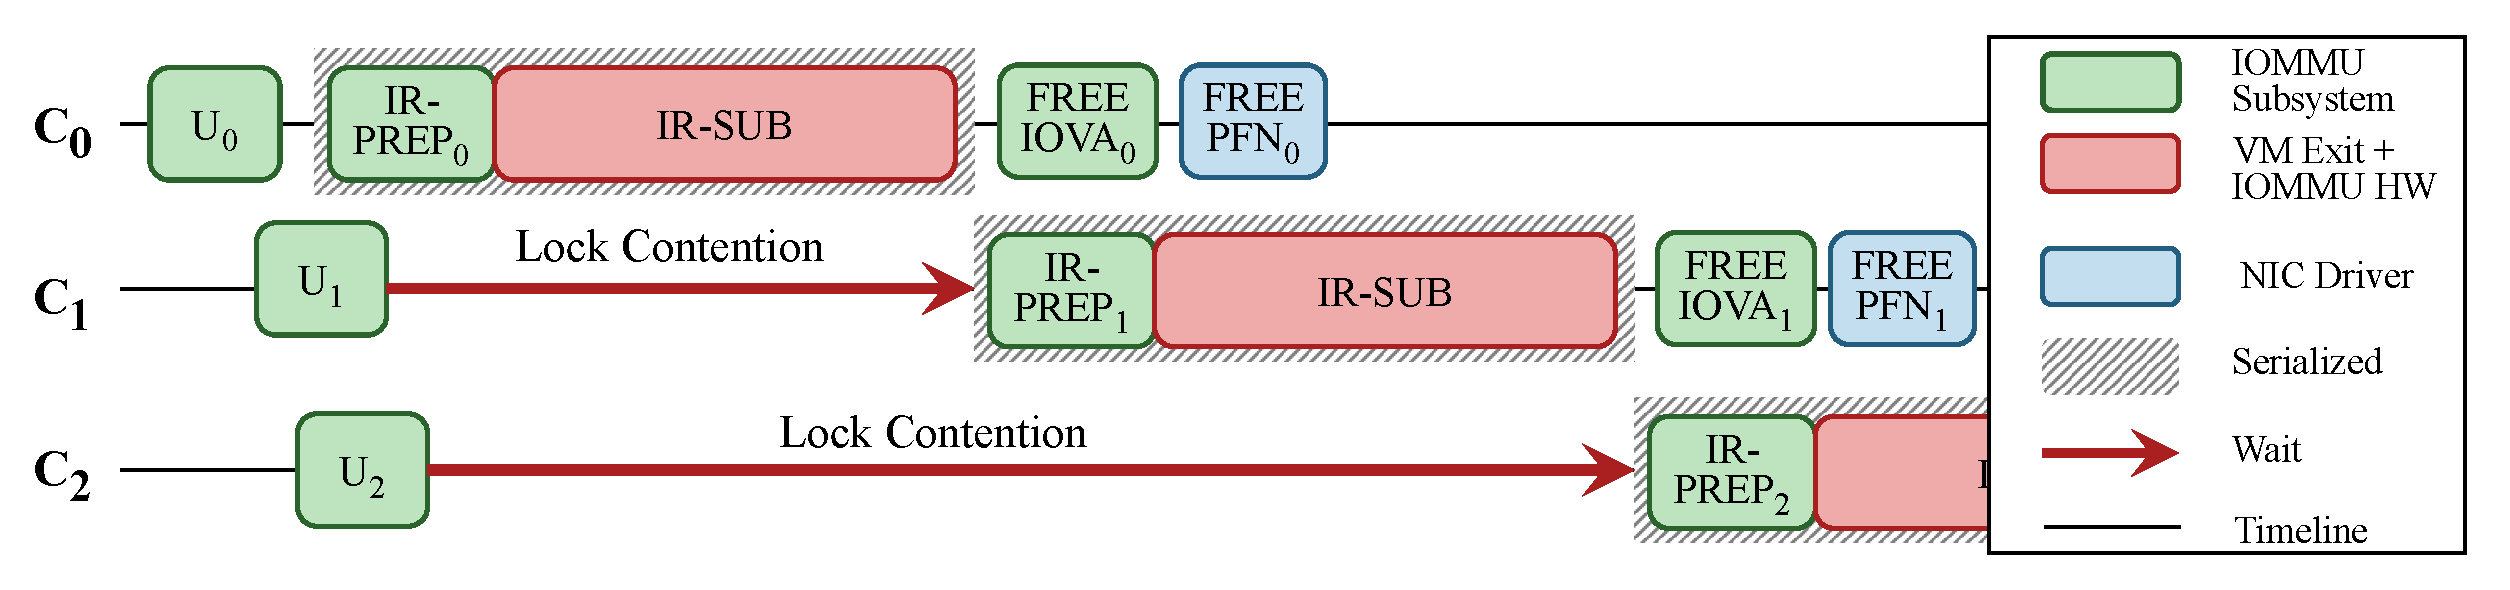
\includegraphics[width=\columnwidth]{figures/strict_serialize_v2_cropped.pdf}
\Description{Serialization in current strict}
\caption{\small {\bf Illustration of strict serialization of each IR-PREP and IR-SUB in existing strict IO memory protection mechanisms across CPU cores ($C_{0,1,2}$).}}
\label{vfree:fig:current-design}
\end{figure}

% \begin{figure}
% 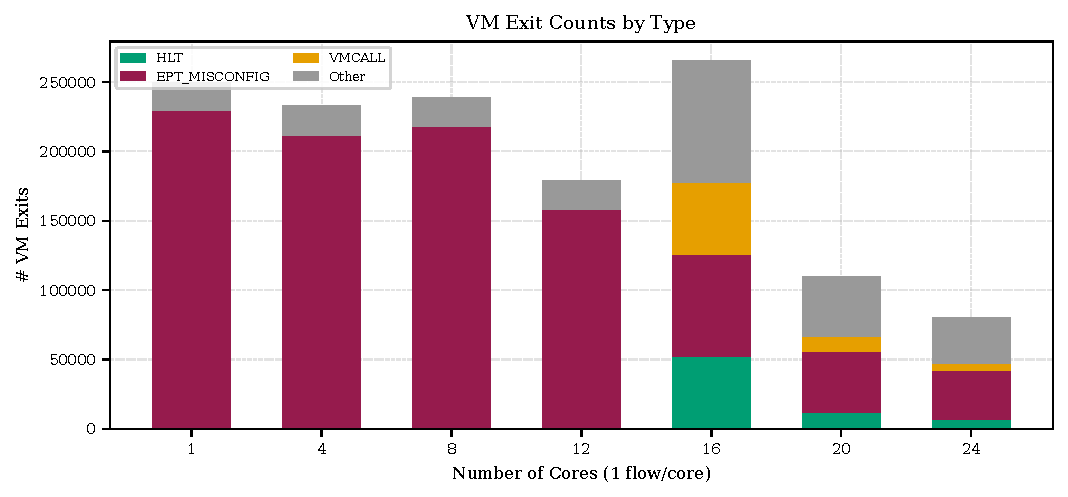
\includegraphics[width=\columnwidth]{figures/vm_exit_counts.pdf}
% \Description{Number of VM exits by exit reason on a single profiled core across increasing core counts. EPT\_MISCONFIG counts decline steadily while PAUSE\_INSTRUCTION, HLT, and VMCALL counts surge between 12 and 16 cores.}
% \caption{VM~exit counts by event type on a single profiled core.
% EPT\_MISCONFIG exits (completed invalidations) decline as contention grows, while PAUSE\_INSTRUCTION and HLT/VMCALL exits surge between 12 and 16~cores}
% \label{vfree:fig:vm-exit-count}
% \end{figure}

% \todo{LESHNA: add pause as separate in vm exit count}

\paragraphb{[Figure~\ref{vfree:fig:lock-contention}] Root cause of throughput reduction at large core counts: % in Figure~\ref{vfree:fig:baseline-iperf}: 
contention-descheduling feedback loop in virtualized environments} We now explain the root causes behind the counter-intuitive observation of throughput reducing with number of cores increasing beyond 12.

% VM exits can happen due to many reasons; Figure~\ref{vfree:fig:vm-exit-time-pct} shows the average time spent on VM~exits on a per \CodeIn{unmap} basis, broken down by events that trigger the VM exit.
% due to all VM exits. 
We observe that two kinds of VM exits dominate. First, VM exits due to MMIO writes to the IOMMU invalidation tail register---``useful work'' of the \CodeIn{unmap} path. Second, VM~exits due to contention-induced vCPU descheduling (triggered by \texttt{HLT} event).
In virtualized environments, an \texttt{HLT} halts a vCPU and triggers a VM~exit that causes KVM to deschedule the vCPU till an interrupt or wake event arrives.

We observe that, at low core counts, nearly all per-\CodeIn{unmap} VM~exit time (${\sim}$94\%) is spent in handling writes to the MMIO invalidation queue tail register 
% in VM exits  due to the \texttt{EPT\_MISCONFIG} event 
and the total per-\CodeIn{unmap} exit cost is ${\sim}$11--18\,$\mu$s (IR-SUB cost in Figure~\ref{vfree:fig:lock-contention}).
At 16~cores and above, contention-induced descheduling consumes
  % \texttt{HLT}-induced VM~exits consume
 {93--97\%} of per-\CodeIn{unmap} exit time, inflating the total cost to 141\,$\mu$s at 16~cores and \textit{514\,$\mu$s} at 24~cores---a $46\times$ increase over the low-contention baseline.
 The reason is as follows.

% \begin{figure}
% 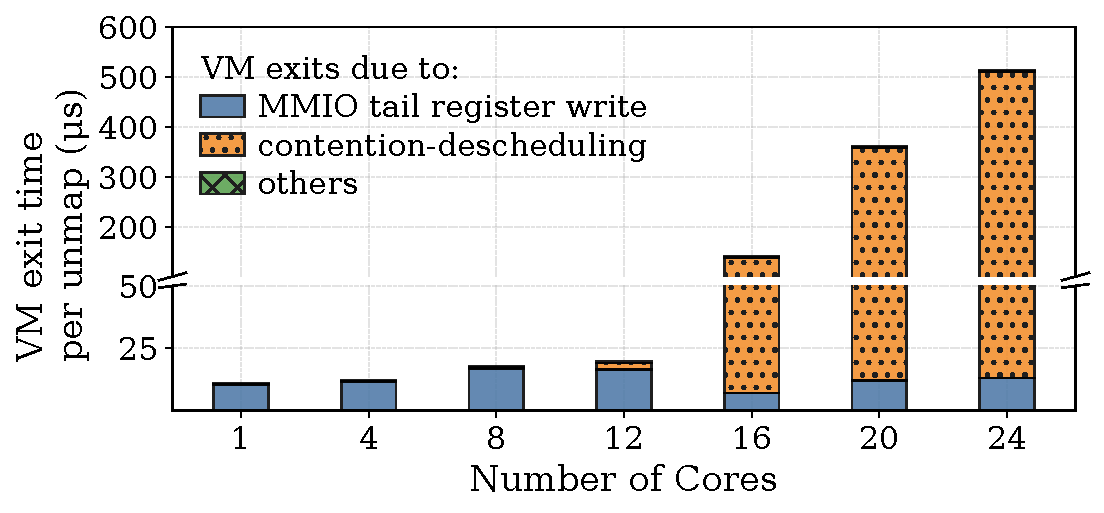
\includegraphics[width=\columnwidth]{figures/vm_exit_time_per_unmap.pdf}
% % \Description{Average VM exit time per unmap operation speant on HLT and EPT\_MISCONFIG across increasing core counts. At low core counts EPT\_MISCONFIG dominates; beyond 16 cores HLT dominates.}
% \vspace{-15pt}
% \caption{\small {\bf Breakdown of average VM~exit time per \CodeIn{unmap} operation due to various events that trigger VM exits.} At low core counts, nearly all per-\CodeIn{unmap} VM~exit time is spent in handling writes to the MMIO invalidation queue tail register; at 16~cores and above, contention-induced descheduling consumes contributes to most of the per-\CodeIn{unmap} exit time. \rachit{make a note on why this figure y-axis has scale higher than figure 5 y-axis scale (why is average HLT time higher than average execution time---the normalization factor for averages uses different number of cores in the two}}
% \vspace{-10pt}
% \label{vfree:fig:vm-exit-time-pct}
% \end{figure}


\para{Contention-descheduling feedback loop.}
The transition from useful work to idle waiting follows a three-stage cascade process visible in the VM~exit data:

\begin{enumerate}
\item {\it Spinning.}
  As vCPU count grows, more vCPUs contend for \CodeIn{cache\_lock}.
  Waiters spin in tight \CodeIn{PAUSE} loops, waiting for the lock holder to complete its invalidation.
  We find that, from 12 to 16 cores,
  \CodeIn{PAUSE}-related VM exits
  increase by {$60\times$}, triggered by the processor's Pause-Loop Exiting (PLE) mechanism,
  which detects sustained spinning and traps to the
  hypervisor once a threshold is exceeded~\cite{Shan2017apples}.
\item \textit{Descheduling.}
  Once a vCPU has exceeded its spin budget,
\if 0
  \footnote{Increasing the 
  PLE spin budget (\textit{i.e.}, \texttt{PLE\_window}) 
  delays the onset of this cascade to higher core counts 
  but does not prevent it: the fundamental throughput ceiling 
  is set by the serialized invalidation path, not by the 
  spin threshold.
  Kashyap et al.~\cite{Kashyap2016oppspinlocks} observe that 
  the collapse simply shifts rightward with a larger budget, 
  and Shan et al.~\cite{Shan2017apples} show that 
  no static threshold is optimal across workloads.},
\fi
  an \CodeIn{HLT} event is triggered, which leads to another VM exit that causes
  the host (KVM) deschedules the vCPU.
  We confirmed that these \CodeIn{HLT}-related VM exits are lock-induced halts, and not due to idle vCPUs. 
  % (the so-called \CodeIn{VMCALL}-induced wakeups~\cite{KVM_KICK_VM_CALL}
  % track almost exactly with \CodeIn{HLT}-related VM exits). 
  The same phenomenon is observed for general kernel spinlocks:
  at a high contention level, most vCPUs
  simultaneously fail their optimistic spin
  and trap to the hypervisor~\cite{Kashyap2016oppspinlocks}.

  
  
  % jump from 588 to 52,265
  % between 12 and 16 cores,
  % tracking \CodeIn{VMCALL} almost exactly
  % (469 to 51,648), confirming these are lock-induced halts, not idle vCPUs.


\item \textit{Expensive wakeup.}
  When the lock holder finishes and
  releases \CodeIn{cache\_lock}, the next waiter must be
  woken via an IPI.
This wakeup path, which is cheap on bare metal (${\sim}$8\,$\mu$s),
  is an expensive event in virtualized environments,
  known as the \emph{Blocked-Waiter Wakeup} (BWW) problem~\cite{Ding2014gleaner}:
  the IPI triggers a VM~exit on the vCPU that triggers the wakeup event, invokes the KVM scheduler,
  and requires a VM~entry to reschedule the target vCPU. The latency for the wakeup path is included in the \CodeIn{HLT} duration.
%  with a penalty factor of 
%  4.6--6.2$\times$ even with dedicated CPU pinning
% BWW arises whenever blocking synchronization 
%  executes in a virtualized environment, 
%  causing increased execution times and reduced 
%  throughput~\cite{Ding2014gleaner}.
In our measurements, average \texttt{HLT} duration per unmap
  grows from $2.5\mu$s at $12$~cores to 131\,$\mu$s at 16~cores to $346\mu$s at 20~cores to $498\mu$s at 24~cores, far exceeding a single BWW event because the cost compounds:
  as more vCPUs are descheduled simultaneously, 
  each must wait longer to be rescheduled,
  and the vCPU responsible for sending wakeup IPIs
  may be contending for the same lock.
% \schaic{
% Do we want the average per call HLT (what we have in the text) or HLT time per unmap (Fig6).}
% During this wakeup window, no core holds the lock.
%  creating idle bubbles on the hardware invalidation queue.
\end{enumerate}
% The three stages form a \emph{positive feedback loop}:
%  contention causes descheduling,
%  descheduling inflates wakeup latency,
%  longer wakeups leave the lock unheld 
%  (introducing pipeline bubbles on the invalidation queue),
%  which increases the effective time between
%  consecutive invalidation completions as seen by
%  all waiting vCPUs---causing more of them to exceed 
%  their spin budgets and be descheduled.
This feedback loop results in {\it super-linear} increase in \CodeIn{HLT}-related VM exit time:
  for the core on which we profile, ${\sim}$157K invalidations are completed for 12~cores
  but only ${\sim}$35K invalidations are completed for 24~cores, a $4.5\times$ reduction with merely $2\times$ increase in number of cores. %---while
%   the average cost of each individual invalidation grows only
%   $1.7\times$ (8.3\,$\mu$s to 14.3\,$\mu$s).
% The remaining ${\sim}3.8\times$ gap
%   is entirely time spent descheduled.

This feedback loop is specific to virtualized environments.
On bare metal, a spinning thread remains on its physical
  core and resumes immediately when the lock is released;
  the virtualization layer converts what would be a brief
  spin-wait into a cascade of VM~exits whose cost compounds
  with every additional contending vCPU.
The individual pathologies---PLE-triggered 
  descheduling~\cite{Shan2017apples}, 
  mass halt under contention~\cite{Kashyap2016oppspinlocks}, 
  and BWW~\cite{Ding2014gleaner, Kashyap2018ecs}---are well studied
  for general kernel spinlocks,
  but the IOMMU invalidation path is a uniquely severe instance:
  the serialized hardware queue is a fixed point
  on every packet's \CodeIn{unmap} that cannot be
  parallelized or avoided.

% \rachit{It would also be nice to show the number of VM exits in Figure~\ref{vfree:fig:vm-exit-time-pct} to further support the evidence.}

% \rachit{if we increased the spin budget, would this phenomenon reduce or even go away for large spin budgets? could we demonstrate that? It would really nail down the problem.} 
% \leshna{added a footnote we can keep if important}
 

\subsection{{\vfreename} Design}
\label{vfree:sec:design}
{\vfreename} is a modification to existing IO memory protection mechanisms
    for {\it strict} intra-VM protection in virtualized environments. {\vfreename} targets the same threat model as Linux strict mode (Appendix~\ref{vfree:sec:threat_model}).
%    that makes strict IO memory protection feasible in virtualized environments.
{\vfreename} achieves this goal using {\em One-for-Many Invalidations} (\S\ref{vfree:ssec:one-to-many}) 
    and {\em Deferred Free Page} (\S\ref{vfree:ssec:dfp}). % This section presents these two ideas.
% the two core design ideas in {\vfreename}: one-for-many invalidations and deferred free page.



% \subsubsection{{\vfreename} Overview}

% % As illustrated in Figure~\ref{vfree:fig:current-design}, the root cause of the performance inefficiencies in existing stacks is serialization of IRs across all threads in the VM. Keeping just one IR in-flight to the IOMMU HW for processing significantly reduces the achievable IO throughput, due to large IR processing latencies (owing to unavoidable VM exits in the datapath; \S\ref{vfree:sec:background-datapath}). In this section, we argue that such a serialized processing of IRs is in fact, completely unnecessary. And building on this insight, we propose {\vfreebrand}---a rearchitecture of memory protection mechanism for virtualized Linux network stacks---that enables concurrent IR processing, while providing strict memory protection. {\vfreebrand} thus helps achieving close-to-no-protection performance (\S\ref{vfree:sec:eval}), while still maintaining the strongest safety guarantees providing by existing stacks (\S\ref{vfree:sec:security}). 


% % {\vfreebrand} achieves its benefits by using two key design ideas, that are complementary to each other. The first idea---Safely Batched Invalidations (SBI)---enables concurrent IR processing by multiple vCPUs in the VM; and the second---Deferred Free Pages (DFP)---enables each vCPU to also concurrently submit multiple IRs for processing. \S\ref{vfree:sec:eval} evaluates the benefits enabled by each idea, and demonstrates that both are necessary to provide near-optimal performance. 

% % SBI is enabled by 



% % % enables concurrent IR processing by enabling each vCPU across the guest to concurrently submit an IR to the IOMMU. 
% % This is enabled by two key ideas: (i) using per-vCPU virtual queues for SW submission queue for safely performing concurrent IR-PREP (ii) decoupling IR-PREP and IR-SUB, to enable batching of multiple concurrent IRs to be submitted via IR-SUB which still needs to be serialized across cores. 

% % % While the first design alleviates the gap between no vIOMMU and strict protection performance, by improving concurrent IRs, specifically 1 by each vCPU, but that's not enough, given the high IR processing latency due to involved VM exits. 


% % The key challenge lies in maintaining strict memory protection under concurrent IR processing. 

% % The second design idea---deferred page frees---enables each vCPU to keep multiple concurrent IRs to the IOMMU HW, enabling to offset the high IR processing latency. This is enabled by performing invalidations asynchronously with unmaps. Performing this without impacting safety is based on the following insight: as long as the following ordering
% % of operations->unmap->invalidate→free page is followed, we
% % maintain the default strict protection guarantees, irrespective
% % (8) We argue this problem is not fundamental: \textit{contrary to conventional wisdom, executing both IR-PREP and IR-SUB synchronously with unmap calls are in fact NOT fundamentally necessary to achieve the strict memory protection.} This tradition fallacy arises due to the way existing network drivers recycle physical physical pages after unmap operations, to be mapped to other IO virtual addresses. The drivers today free a physical page after every unmap call. To ensure strict protection, we need to invalidate the IOTLB before the physical page is freed and recycled (or else it could result in known confidentiality attacks~\cite{}). Therefore, today invalidations are performed synchronously with unmaps to ensure they are always executed before the corresponding page free operations. Our key insight is that \textit{as long as the following ordering of operations---unmap$\rightarrow$invalidate$\rightarrow$free page is followed, we maintain the default strict protection guarantees}, irrespective of the fact whether invalidations are synchronous with the unmaps. \saksham{probably need to mention somewhere that recent linux kernel designs also ensure that there is no possibility of TOCTOU attacks even with asynchronous unmaps and invalidations.}
% % of the fact whether invalidations are synchronous with the unmaps. 

% % /** Current System */

% % lock (cache\_lock) // per domain

% % SUBMIT INV req to SW queue

% % lock (q\_lock) // per device

% % pick the request from the SW q and send to the HW q

% % PROCESS INV req

% % unlock(q\_lock)

% % unlock(cache\_lock)


% % /** Our Work */
% % // change per-domain cache\_lock to per-CPU cache\_lock

% % // change per-domain SW queue to per-CPU SW queue

% % // remove nested locking

% % lock(cache\_lock) // per CPU

% % SUBMIT INV req to SW queue

% % unlock(cache\_lock)

% % lock(q\_lock)

% % pick the request from the SW q and send to the HW q

% % PROCESS INV req

% % unlock(q\_lock)

% % \rachit{are we sure the above is correct?}
% % \subsubsection{Thoughts/Flow}

% % we decouple IR-PREP and IR-SUB; 

% % if we don't decouple, nothing fundamentally changes---we don't reduce the number of VM exits; 

% % \subsubsection{Preparing Invalidation Requests {\em Before} Cross-Core Serialization [\saksham{Will get rid of this subsection}]}

% % \begin{itemize}
% %     \item We want to reduce number of VM exits per unmap; today it is strictly more than 1, due to cross-core serialization before IR-PREP---prohibiting any opportunity to ``batch'' IRs to be submitted to the hardware via a single write to the invalidation queue, i.e. a single VM exit \rachit{for each point being made here, there should be a direct subsection/paragraph in S3 that we should be able to point to;} \rachit{we are mixing the goal with the solution: do not bring up batching; that is part of the solution}

% %     \item Such cross-core serialization today is performed to prevent concurrent reads and writes to per-IO-domain data structures; reads are performed during IR-PREP operation, writes are performed to allocate/deallocate the data structures during IO device attach/detach events. \rachit{could we point back to S2 where we discuss these?}

% %     \item We argue that performing cross-core serialization {\em before every} IR-PREP operation is unnecesarily aggressive, due to two reasons: (i) while concurrent reads and writes need to be serialized, there is no need to serialize concurrent reads; and (ii) attach/detach are rare events 

% %     \item We propose eliminating the cross-core serialization before IR-PREP, and only serialize reads and writes: {\em only when} attch/detach is happening, no thread can perform IR-PREP; otherwise concurrent threads can perform IR-PREP; since writes are rare events in practice, we most often see no serialization/blocking across cores to perform concurrent IR-PREP. \rachit{this is a bit confusing and if written this way will introduce questions related to safety guarantees: I suggest to describe it as {\vfreebrand} introducing a slow path and a fast path for IR-PREP: the former is triggered when attach/detatch happen and require cross-core serialization; the latter requires no cross-core seralization (common case)}  

% %     \item However, cross-core serialization is still required after IR-PREP: IR-SUB operation needs to be serialized---since it perfoms write to single emulated HW q (can't have multple emulated qs without modifyind the hypervisor); so serialization is necessary before IR-SUB; 

% %     \item Hence, our key design idea is to move cross-core serialization to after IR-PREP and before IR-SUB. Essentially, this design decouples IR-PREP and IR-SUB operations---i.e., they are no longer performed within the critical section of a same lock. Cross-core lock is only acquired before IR-SUB operation. 

% %     % \item If we need to reduce the number of VM exits per unmap, we need to perform a single VM exit for multiple IRs; that necessitates decoupling IR-PREP and IR-SUB; 

% %     % \item After concurrently preparing IRs, cross-core serialization is done to enqueue the requests to a single logical SW Q---enabling "batching" (need to be careful with the term); 
% % \end{itemize}
% % \rachit{high-level feedback: IR-PREP overheads do not even show up in Figure 6 and 7: why are we spending so much time and real estate discussing IR-prep?}

% {\vfreename} enables multiple vCPUs to concurrently prepare IRs for submission to the IOMMU; the vCPUs then remain blocked until invalidation is completed. For all invalidations requests concurrently prepared across different vCPUs, {\vfreename} enables actually submitting only a single IR descriptor to the IOMMU hardware in a manner that executing the single submitted invalidation request results in invalidating the IOMMU cache entries for all invalidation requests. Recall that submitting an IR descriptor to the emulated invalidation queue results in an unavoidable VM exit. Hence, using a single submission for multiple IRs reduces the number of VM exits to only one for entire set of concurrent requests (instead of one VM exit for each individual request as today). 

% We use two key insights to realize one-for-many invalidations. The first insight is to decouple the IR processing pipeline (IR-PREP and IR-SUB operations discussed in \S\ref{vfree:sec:background-datapath}) across multiple threads, each using separate independent locks. This allows multiple vCPUs to concurrently perform IR-PREP operations to prepare requests while IR-SUB is concurrently executing on another thread. The second insight enables performing invalidation for the multiple prepared IRs using only a single submission to hardware. We achieve this by sending an IR with a special flag that {\em flushes all IOMMU caches} for the VM. While flushing the IOMMU caches can increase address translation overheads (due to larger IOPT lookup overheads owing to IOMMU cache misses~\cite{Rubin2024FastSafe}; \S\ref{vfree:sec:background-datapath}), increasing address translation overheads to reduce the number of VM exits turns out to be a good tradeoff. 

% While one-to-many invalidations enable multiple vCPUs to concurrently prepare IRs, each vCPU still remains blocked upon preparing a single IR until invalidation limiting the performance benefits. This is done to guarantee strict safety since the IOVA and the corresponding physical page must be released for future reuse only after completing invalidation. {\vfreename}'s second design idea of deferred free page addresses this challenge: {\vfreename} ensures that each page is freed only after the corresponding invalidation has been completed. Using this idea, vCPUs are not blocked and can continue preparing more IRs even while the previous IRs have not been invalidated. The key insight here is as that long as physical pages are freed only after their corresponding IOVAs are invalidated, strict safety is guaranteed. 

% The next two subsections describe the two ideas in detail; we then discuss how {\vfreename} maintains strict safety guarantees (\S\ref{vfree:sec:security}).

% \begin{itemize}
    


%     his is because, to
% guarantee strict safety, the IOVA and the physical page must
% be released for future use only after the invalidation has
% completed [? ? ? ]. To that end, the deferred free page idea
% delegates free IOVA and free page operations to the dedi-
% cated vCPU, which performs these operations only and im-
% mediately upon receiving the completion signal.

    % \item The second idea is deferred free page
% \end{itemize}
\subsubsection{Enabling Concurrent Invalidation Requests}
\label{vfree:ssec:enabling}
As discussed in \S\ref{vfree:sec:background-datapath}, 
    existing IO memory protection mechanisms 
    enforce strictly one invalidation requests (IR) in flight: 
    vCPUs acquire the \CodeIn{cache\_lock} before executing IR-PREP, 
    synchronously execute IR-SUB, and release the lock only after the IR completion signal is received; 
    during this process, all other vCPUs remain blocked, waiting to prepare and submit their respective IRs. 
Since each IR requires a VM exit, existing IO memory protection mechanisms 
    enforce at least one VM exit per IR to enable strict IO memory protection.

\para{Fast path for concurrent IRs.}
{\vfreename} enables a fast path within IO memory protection mechanisms that 
    allows keeping multiple in-flight IRs. 
To achieve this, {\vfreename} decouples the two operations involved in IR processing---preparing 
    IR descriptors (IR-PREP) and submitting the descriptors to the hardware (IR-SUB)---across multiple threads. 
Specifically, {\vfreename} uses a producer-consumer model, as shown in Figure~\ref{vfree:fig:async-design}. 
IR-PREP is executed by producer threads---which are the same threads performing unmap operations. 
Furthermore, {\vfreename} replaces the single IO-domain queue and \CodeIn{cache\_lock} 
    with per-CPU virtual IO-domain queues, each protected with per-CPU \CodeIn{cache\_locks}. 
This allows multiple producer threads (running concurrently on multiple vCPUs) 
    to concurrently execute IR-PREP: 
    each producer acquires its per-CPU \CodeIn{cache\_lock}, 
    prepares an IR, enqueues it in per-CPU virtual IO-domain queue, releases the per-CPU \CodeIn{cache\_lock}, and then waits to receive a completion signal for its IR. 
With this design, multiple IRs can be kept in flight. %producer threads across vCPUs can now concurrently execute IR-PREP. %In fact, our measurement results in Figure~\ref{vfree:fig:lock-contention} establish that IR-PREP is a light-weight operation. To run IR-PREP, the thread first acquires the \CodeIn{cache\_lock}, enqueues the prepared IR descriptor in the {IO-domain queue}, and then immediately releases the \CodeIn{cache\_lock}.

The IR-SUB operation is executed by a consumer thread on a designated core. % (the highest-numbered online core).
% For design simplicity, the consumer thread runs on a dedicated vCPU by default (we discuss an optimization in \S\ref{vfree:sec:impl} 
%    that allows the consumer thread to run in a distributed manner without any dedicated vCPU). 
The consumer thread acquires each per-CPU \CodeIn{cache\_lock} one at a time, 
    copies pending IR descriptor(s) from the per-CPU IO-domain queue to a temporary buffer, 
    and immediately releases the per-CPU \CodeIn{cache\_lock}. 
%--- the IR-SUB operation always executes there.
% \review{
When a producer observes that its IR has not completed, 
    it attempts to activate the consumer by atomically test-and-setting a domain-wide BUSY bit.
If the test-and-set succeeds, the consumer is inactive; thus,
    the producer schedules the consumer on the designated core
    via a workqueue.
    % via a high-priority workqueue running in softirq context.%
% \footnote{We chose a workqueue over SMP function calls because the latter would execute in hard-interrupt context,
% which cannot invoke DFP callbacks with NAPI optimizations~\cite{linux_napi,mlx5_napi_poll} \rachit{we have not introduced DFP yet}}
If the test-and-set fails, the consumer is already running;
the producer spins on the completed counter until the consumer finishes.
If the producer is running on the designated core
(dispatching via the workqueue would deadlock), %since the target core is occupied by the producer itself.
    the producer executes the flush locally, bypassing the workqueue.


% \rachit{the rest of the paragraph should move to the next subsection}
% Only after processing all per-CPU virtual IO-domain queues, the consumer thread acquires the \CodeIn{q\_lock}, copies the descriptor from the buffer to the emulated HW queue. It then notifies hypervisor to perform invalidation by writing 
% to the MMIO invalidation queue tail register (incuring a VM exit); it releases the \CodeIn{q\_lock} only upon the invalidation completion. 

\begin{figure}[H]
	\centering
% 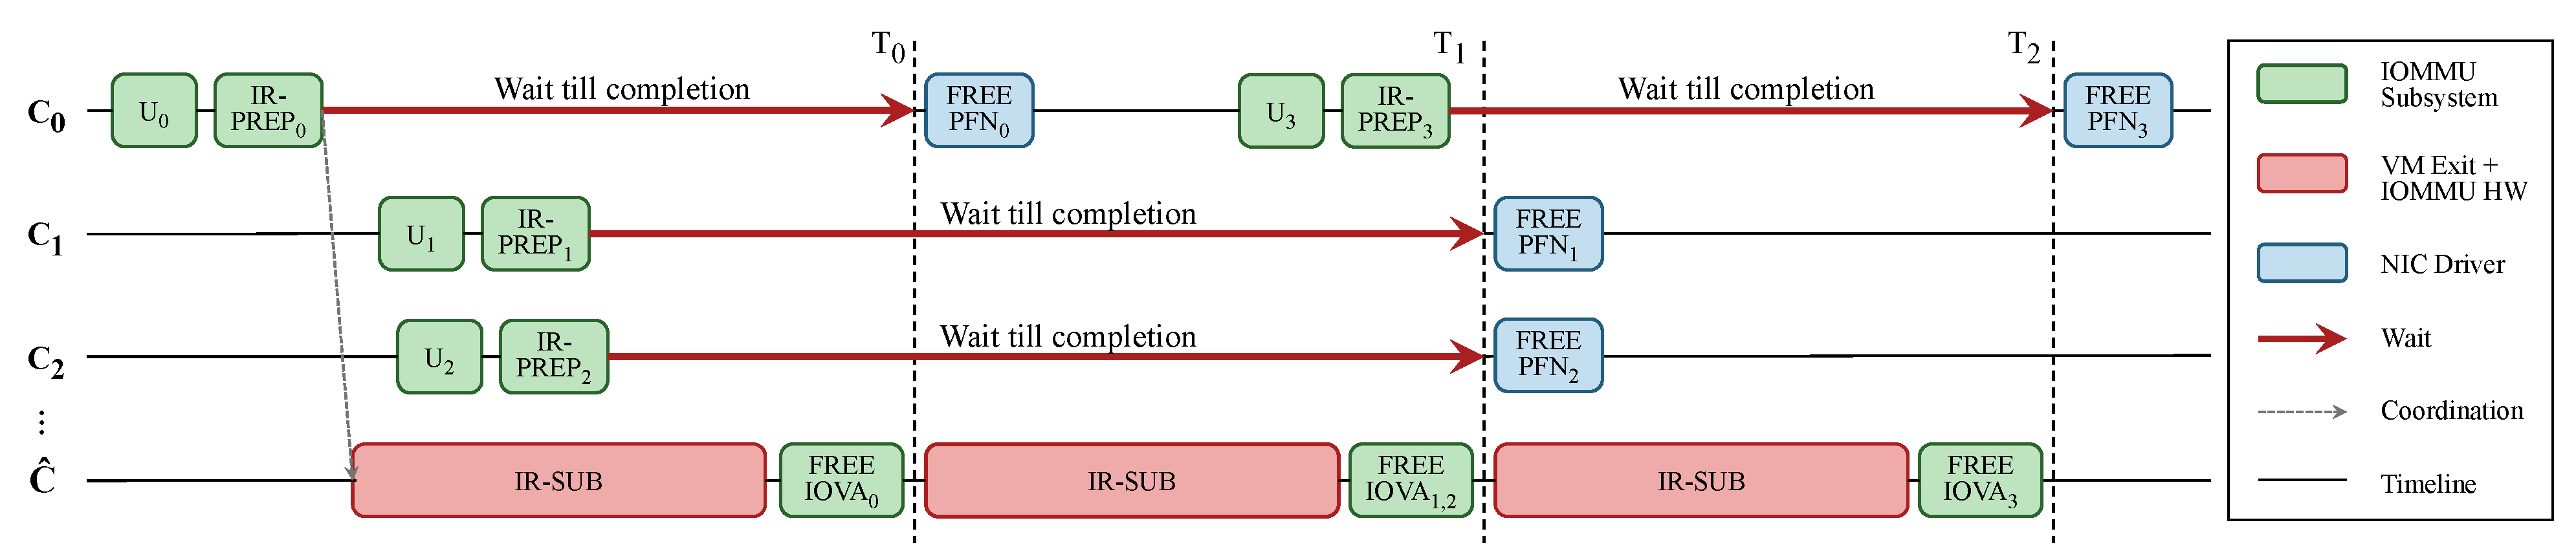
\includegraphics[width=\linewidth]{figures/omf_v4_cropped.pdf}
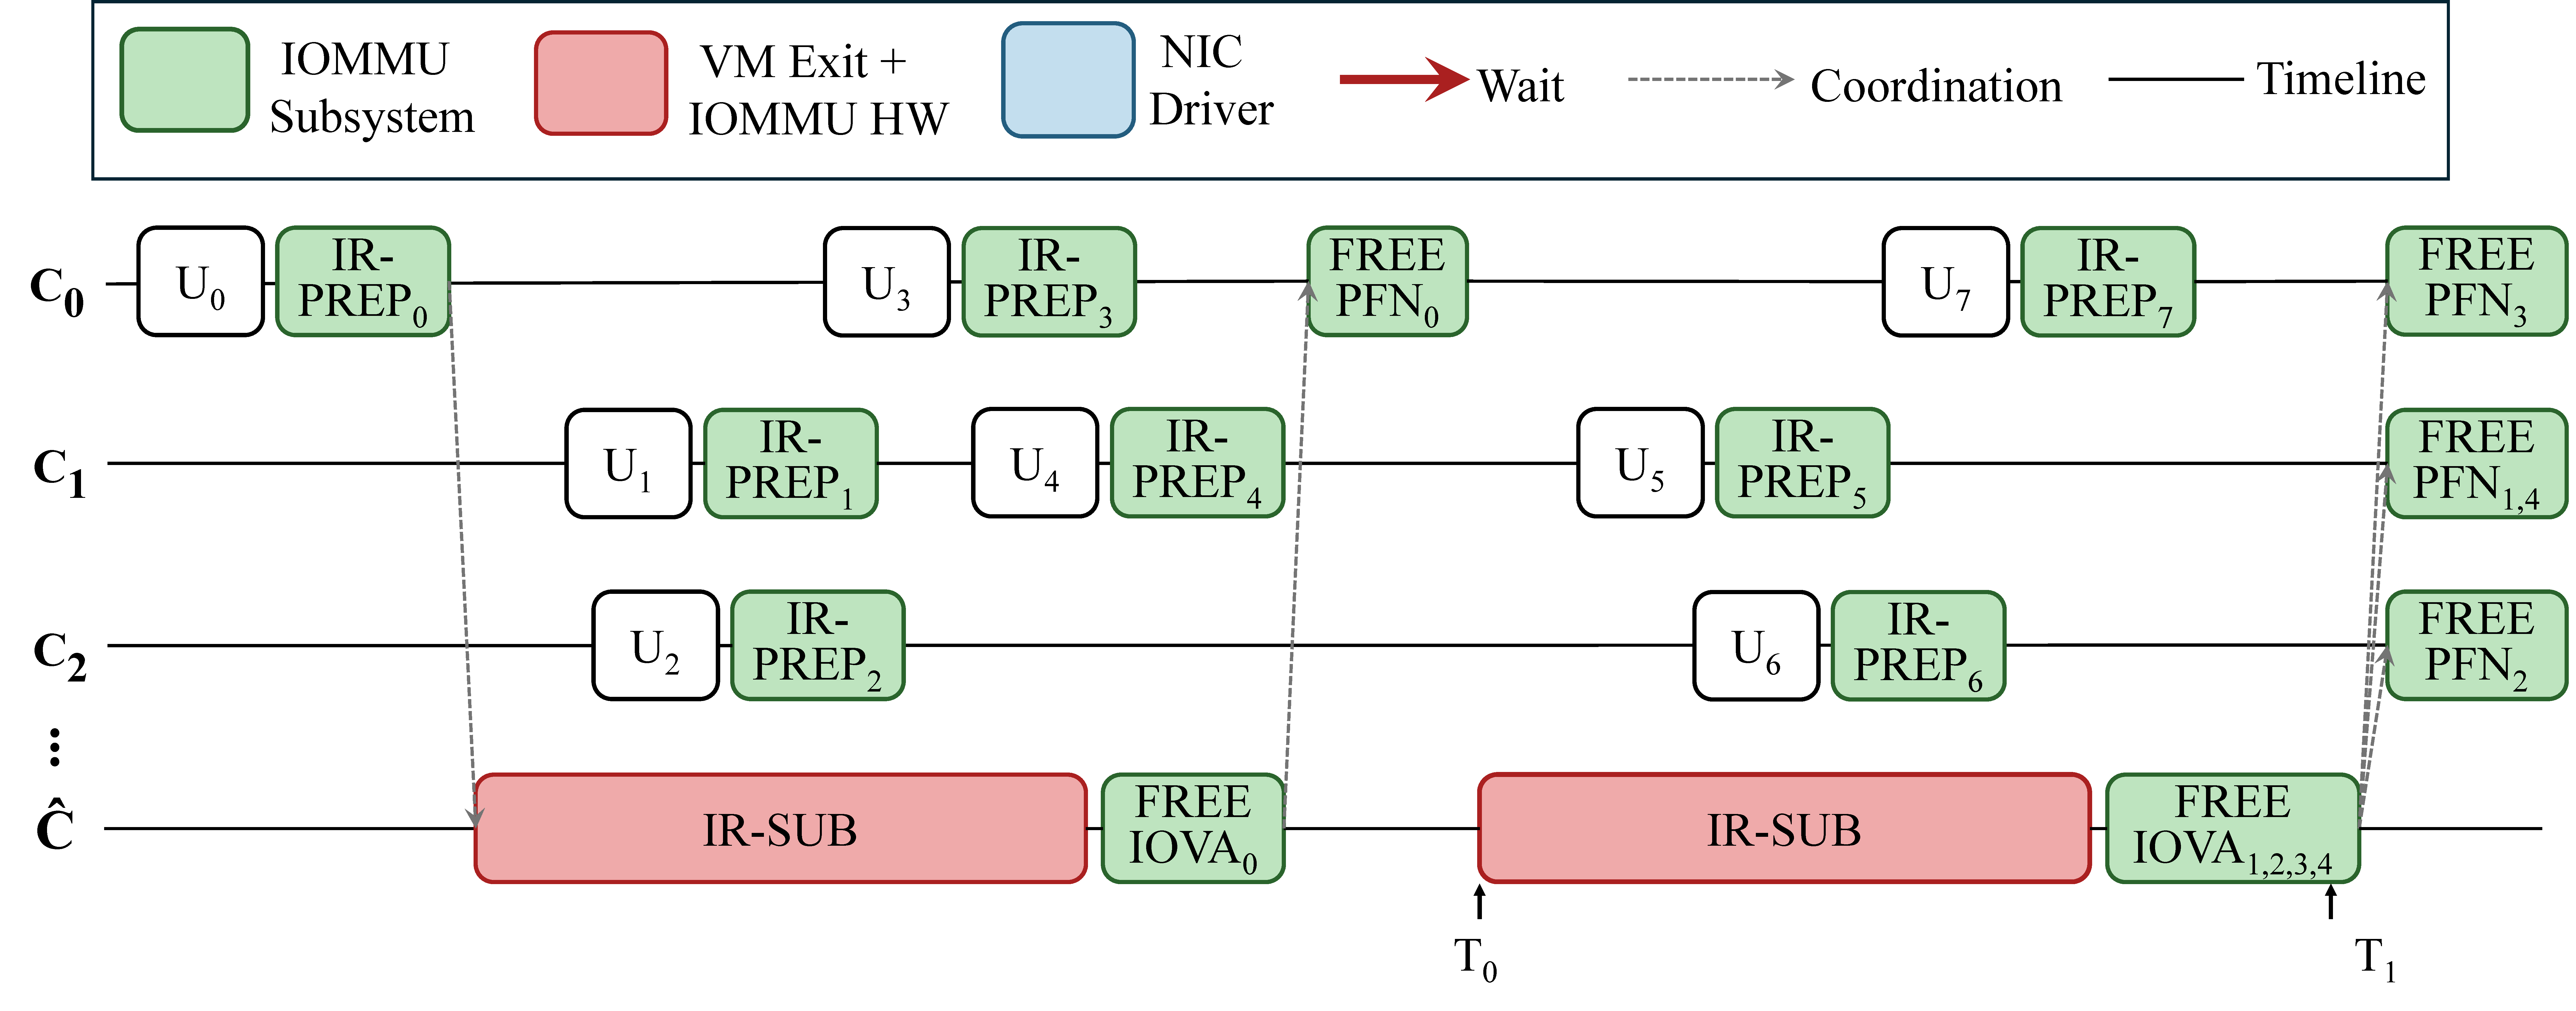
\includegraphics[width=\linewidth]{figures/One_for_many_timline.pdf}
\caption{\small
    \textbf{
One-for-many enables multiple IR-PREPs to run concurrently with an IR-SUB operation. 
It reduces the number of VM exits by using one IR-SUB operation
for all outstanding IRs to flush all IOMMU caches.}
In this figure, producers run on cores $C_1, C_2, C_3$, and a dedicated consumer thread runs on $\hat{C}$.
Each producer performs an unmap operation (U$_{1-3}$) and busy-waits until its IR is invalidated by the consumer thread.
}
% \saksham{We need to show the pinned version here instead; showing consumer thread running on 1 core, and producers on others; }\saksham{we should club copy as part of IR-SUB}}
\label{vfree:fig:async-design}
\end{figure}

% \para{Per-CPU queue for IR-PREP.}
% We improve the scalability of \vfreebrand
% by replacing the single IO-domain queue and \CodeIn{cache\_lock}
%     with per-CPU queues protected by per-CPU locks.
% % The per-CPU SW queue is protected by a per-CPU lock.
% The optimization enables multiple producers to execute IR-PREP in parallel.
% With the per-CPU queue,
% each producer acquires its per-CPU lock,
% prepares an IR and enqueues it.
% After the short IR-PREP (As shown in Figure~\ref{vfree:fig:lock-contention}), the producer releases the lock.
% This optimization avoids multiple producers contending for the per-IO-domain \CodeIn{cache\_lock} 
%     at IR-PREP time,
%     which could lead to long lock contention especially when DFP is enabled. \leshna{quick explaination as of why}

% The consumer copies all IRs from all per-CPU queues to a temporary buffer.
% It grabs the per-CPU lock one by one, and releases it after each copy.
% % The consumer never holds more than one per-CPU lock at a time.
% % it acquires the per-CPU lock,
% % rather than contending for the per-IO-domain \CodeIn{cache\_lock} a per-IO-domain SW queue.
% % The per-CPU SW 
% % % a per-CPU SW queue rather than a per-IO-domain SW queue.
% % After the producer core unmaps an IOVA, it acquires only its own per-CPU lock, prepares an the request based on given IOVA range, 
% % and appends the IR to its per-CPU SW queue.
% The per-CPU lock is released before IR-SUB,
%     enabling other producers to prepare more IRs while the consumer performs IR-SUB.

% \paragraphb{Slow path for maintaining strict IO memory protection}
\para{Slow path.}
As discussed in \S\ref{vfree:sec:inefficiencies}, IO memory protection mechanisms 
    use \CodeIn{cache\_lock} to protect cache tags for each IO-domain, as
    a domain can be attached/detached at any time, and the list of cache tags is recycled during invalidation.
% With our per-CPU design,
% This is a more expensive operation than acquiring a single per-IO-domain lock,
The domain attaching/detaching is a rare event, but must be accounted for to maintain strict IO memory protection. 
Thus, any domain attaching/detaching event triggers the slow path: \emph{all} per-CPU \CodeIn{cache\_locks} 
    have to be acquired at attaching/detaching time to ensure safety.

\subsubsection{One-for-Many Invalidations}
\label{vfree:ssec:one-to-many}
% \saksham{todo---we'll be mentioning one-for-many itself as the first key design idea; rethink how the two concepts below are introduced, not as two design ideas again}
% \saksham{Todo: avoid using the word "(a)synchronous"}
% \schaix{
% , and then releases the \CodeIn{q\_lock} upon receiving write completion.
% % }
% \schai{
% It then acquires the \CodeIn{q\_lock}, copies the descriptor from the buffer to the emulated HW queue, 

% The VM exit is triggered at MMIO write time.
% The MMIO write triggers a VM exit to doorbell the hypervisor 
% pass the invalidation request to host OS and utimately invalidating the physical IOTLB or IOPT caches.
% }
% followed by MMIO write to the invalidation queue tail register to 

% each preparing IR descriptors and enqueueing to a shared, per-IO-domain, \CodeIn{sw\_queue}. 

% Specifically, we propose performing IR-PREP and IR-SUB operations independently, in separately acquired locks 

% \saksham{todo: Some details on producer/consumer design here to enable decoupling; say IR-PREP is performed by the producer threads---same thread performing unmap, after IR-PREP; a dedicated consumer thread for IR-SUB, AND ALSO freeing the corresponding IOVAs}

% (shown in Figure~\ref{vfree:fig:decoupled-design}\saksham{Todo: add figure}).



% Such decoupled IR processing enables a useful design opportunity which can help reduce the number of VM exits per unmap. This is because the decoupled design allows concurrent 
Decoupling IR-PREP and IR-SUB processing across producer and consumer threads enables 
    {\vfreename} to execute them concurrently. 
Recall that the majority time of IR-SUB 
    is spent for the VM exit, 
    which is executed within the \CodeIn{q\_lock}; 
IR-PREP requires only acquiring the per-CPU \CodeIn{cache\_lock}, and can therefore be executed concurrently. 
Executing multiple IR-PREPs concurrently during an ongoing IR-SUB enables generating multiple IR descriptors 
    by the time this IR-SUB operation finishes. 
The one-for-many invalidations technique in {\vfreename} exploits this opportunity 
    to efficiently reduce the number of VM exits per unmap operation.

% This presents an opportunity to submit a single representative IR descriptor to the hardware that can collectively invalidate all IOVAs in the group of IRs.  %needed for invalidations from $N$ to 1. 
% \saksham{Do we need to discuss the tradeoff here, that we need to acquire the cache lock again to read the IR from SW Q to copy to HW Q, but its a good tradeoff to make due to reduced VM exits?}
    

\para{Flushing IOMMU caches to enable one-for-many invalidations.} 
The (emulated) IOMMU invalidation queue supports submitting 
    multiple IR descriptors---up to 256 entries in our setup---before updating the tail register. 
It is possible to use this interface to submit all outstanding IRs with a single tail register update (and hence a single VM exit); 
this will invalidate the IOMMU cache entries corresponding to the outstanding IRs. 
The invalidation queue in existing hardware only supports invalidating a contiguous IOVA range 
    for any enqueued IR descriptor~\cite{intel_scalable_iov_spec}. 
However, the group of IR descriptors to be invalidated can be arbitrarily discontiguous 
    collectively\footnote{Existing works~\cite{Rubin2024FastSafe} have studied reasons 
        for discontiguity in IOVAs allocated even for successive maps.}.
Thus, when submitting multiple descriptors together to the invalidation queue, 
    the total time to invalidate IOMMU caches will scale with the number of entries submitted. 
Specifically, IOTLB invalidation cost is known to be ${\sim}{600}$-${700}$ns~\cite{Malka2015rIOMMU}
% \saksham{Siyuan, might be nice if we can measure on our server}. 
Hence, the overhead of performing multiple invalidations, one for each outstanding IR, will at least be a few microseconds.

{\vfreename} executes only one IR for all outstanding IRs, 
    but invalidates the {\em entire} IOVA address space for each IR-SUB operation, 
    independent of the IR group size or IOVA ranges the IR group represents. 
This is feasible today via a special IR descriptor type that 
    {\em flushes} all IOMMU cache entries associated with the guest\footnote{IOMMUs today provide 
        per-guest isolation in caches by using separate PASIDs for each guest~\cite{Zhang2024HDIOV}}. 
% \saksham{Mention here we flush only the caches associated with the guest; there is per-guest isolation in terms of caches}
%
% submits a single representative IR descriptor to the IOMMU invalidation queue, along with a flag requesting the hypervisor to flush all IOMMU caches for the corresponding VM. we argue that flushing the IOMMU caches still provide a better trade-off. 
%
Flushing the IOMMU caches maintains correctness guarantees---\textit{i.e.}, the IOVAs represented by 
    the group of IRs will be invalidated. 
Thus, the submitted IR acts as a {\it one-for-many} invalidations: 
    the single submitted IR results in invalidating the IOMMU cache entries for all outstanding IRs. 
This reduces the number of VM exits by the same factor as the number of outstanding IRs. 
However, flushing the IOMMU caches also poses an inherent tradeoff: 
    while VM exits per unmap and invalidation decrease, the address translation cost may 
    increase (see phase 2 in \S\ref{vfree:sec:background-datapath}). 
This is because after flushing IOMMU caches, subsequent IOVA-to-HPA lookups may take as many as $4$ memory accesses, 
    instead of potentially $1$--$4$ depending on cache hit rates~\cite{Rubin2024FastSafe}. 
% \saksham{Revisit this given 2-level translation, and end-to-end translation, i.e., IOVA-to-HPA kept in IOTLB can also be lost; could be more than 3 extra accesses.}
This is a strictly good tradeoff to make: even in the extreme case 
    where we incur three extra memory accesses for address translation, 
    assuming a pessimistic memory access latency of $100$ns, 
    it will cost ${\sim}3\times100$ns extra overhead. 
This is much smaller than a VM exit overhead, which can be several $\mu$s (10--12$\mu$s in our measurements).  
Moreover, larger sized IR groups being invalidated using a single flush (which will be the case in the high network load case) result in larger gains. 
    % \vspace{0.1in}
    % \paragraphb{Using one-for-many invalidations in {\vfreename}}
    % We next describe how {\vfreename} builds upon the two key insights discussed above to minimize VM exits per unmap, while maintaining the same safety guarantees as strict memory protection in Linux. 

\begin{figure}[H]
	\centering
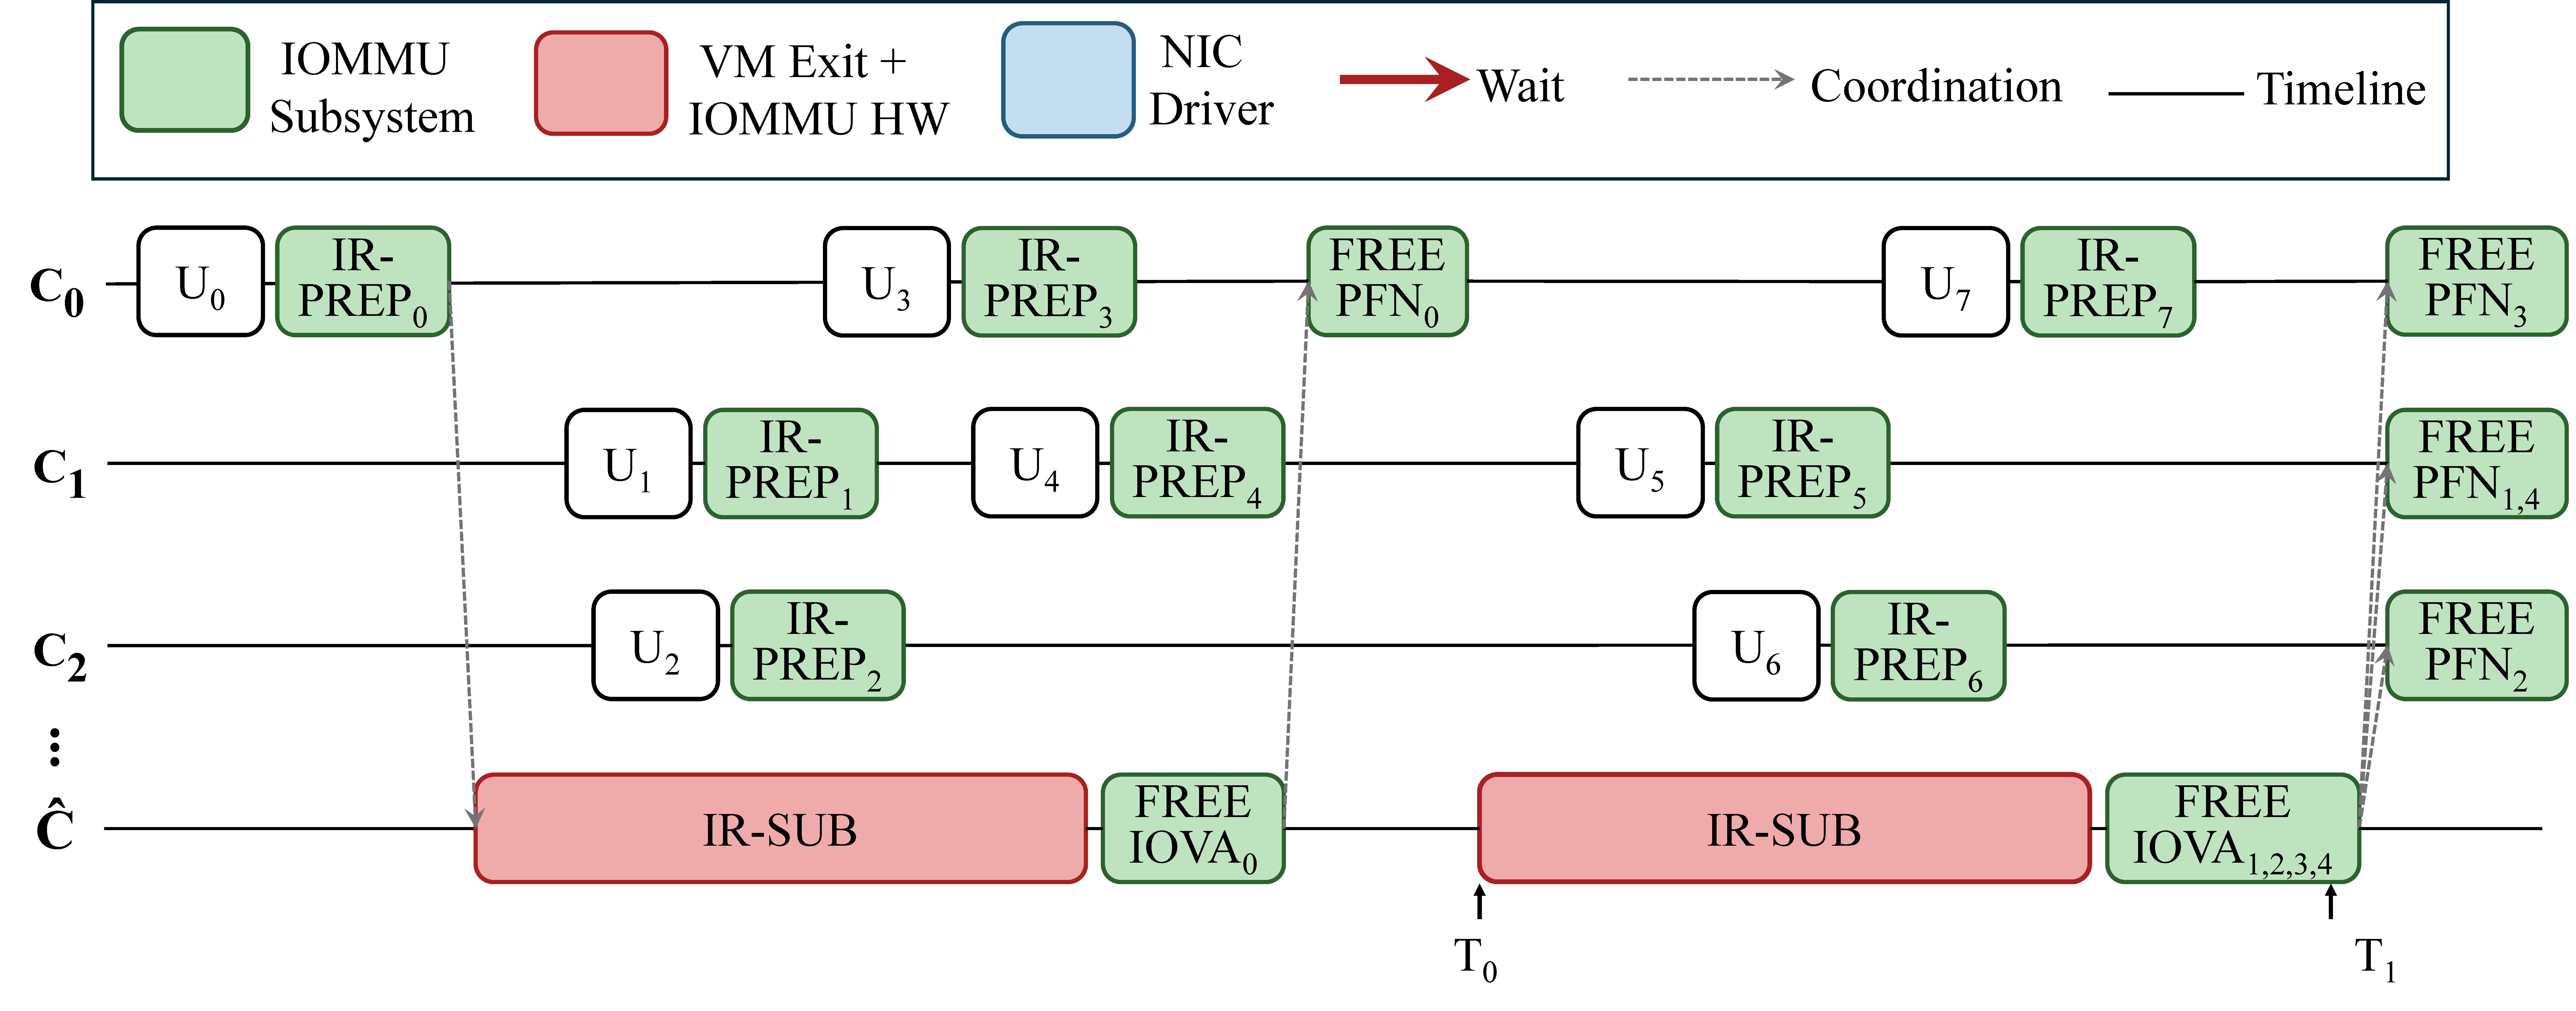
\includegraphics[width=\linewidth]{figures/dfp_timeline.pdf}
% 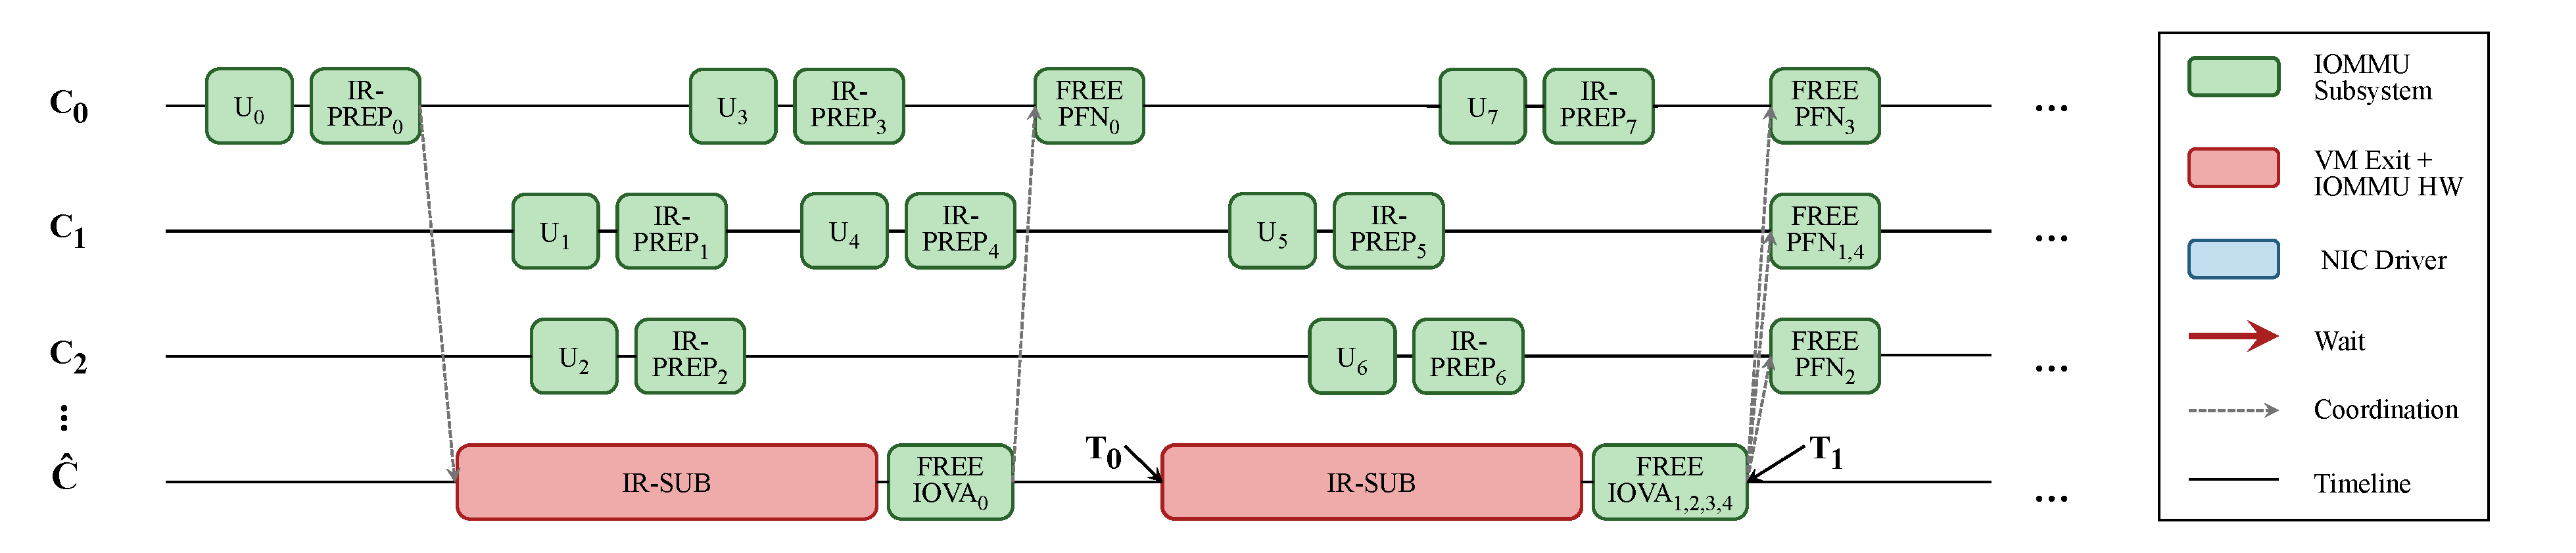
\includegraphics[width=\linewidth]{figures/dpf_side_cropped.pdf}
\caption{\small
    \textbf{
With deferred free page, vCPUs
can proceed immediately without waiting for the invalidation to complete.}
In this figure, producers run on cores $C_1, C_2, C_3$ and dedicated consumer runs on $\hat{C}$.
Each producer thread performs unmap (U$_{1-3}$) and IR-PREP operations and immediately proceed.
It enforces strict protection by deferring the free page operation to after the IR-SUB operation completes.
}
% \saksham{Copy is part of IR-SUB the way I've currently defined in text; one thing needs to update.}}
\label{vfree:fig:dfp}
\end{figure}

    % \paragraphb{An example}
Figure~\ref{vfree:fig:async-design} illustrates the one-for-many invalidation design: 
    each producer, upon any {unmap}, executes IR-PREP. Next, there are two cases. 
First, if the consumer thread is inactive (such as for {\tt IR\_PREP$_0$} in Figure~\ref{vfree:fig:async-design}), 
    % \schaix{the producer thread wakes up the consumer and asks it to perform IR-SUB.}
    {the producer thread schedules the consumer thread on a designated vCPU.} 
    % \schaix{Upon waking up,} 
    The consumer copies IR descriptors from each of the per-CPU virtual IO-domain queues, 
    acquires the \CodeIn{q\_lock}, copies one of the IR descriptors with the flush-all flag, 
    and then writes to the MMIO invalidation queues tail register (incurring a VM exit); 
    the consumer then busy waits until it receives the invalidation completion signal; 
    upon receiving the signal, it frees IOVAs contained in the IR descriptors copied from the per-CPU virtual IO-domain queues. 
Or,  
    % \noindent
    % (2) 
    if the consumer thread is active, running IR-SUB for previously prepared IRs (such as  {\tt IR\_PREP$_1$} in Figure~\ref{vfree:fig:async-design}), the IR will be submitted by consumer's next round of operations. When any round of consumer operations finishes, the consumer starts executing another round if there are any descriptors present in the per-CPU virtual IO-domain queues. 
    % \schaix{Otherwise, it goes to sleep.} 
    {Otherwise, it terminates.} 
    % \schaic{The change here doens't impact the design story, what I added is what we actually have.}

   
    % When the current IR-SUB operation finishes, 
    %     the consumer core collect all IRs from all producer cores' SW queues, perform a single IR-SUB (single VM exit) that flushes all IOPT caches for the domain,
    %     and free the IOVAs based on all IRs.
    % Otherwise, if an IR-SUB operation is ongoing concurrently, the thread remains blocked until the IR-PREP. 
    
    Importantly, each producer thread also {\em busy waits} until its IOVA has been successfully invalidated and freed by the consumer. For instance, producer thread $P0$ waits until time $T0$, and $P1,P2$ wait until time $T1$ in Figure~\ref{vfree:fig:async-design}. This is required to maintain strict IO memory protection with existing network drivers. The drivers today free a physical page after every unmap call (shown in blue color in Figure~\ref{vfree:fig:async-design}). To ensure strict protection, we need to invalidate the IOMMU caches before the physical page is freed and recycled; or else it could result in known integrity and confidentiality attacks~\cite{RajapakshaIOMMU}. 
    % \saksham{Come back here after reading safety subsection}
    % Therefore, today invalidations are performed synchronously with unmaps to ensure they are always executed before the corresponding page free operations---as is the case with this proposed design.
    
\para{Preserving strict IO memory protection.}
One-for-many invalidation preserves the invariant required for strict IO memory protection---each core still blocks until 
    its own invalidation request (IR) completes before freeing the page.
What changes is \emph{when} the invalidation descriptor is submitted to the IOMMU hardware, 
    {\it not} the order between IR completion and page free.
% Under vanilla strict mode, each core acquires the global lock, submits one invalidation descriptor, busy-waits for hardware acknowledgment, and only then proceeds to page free.
% Under \optOne, the core still submits its invalidation descriptor and still waits for hardware acknowledgment before proceeding---the difference is that the lock is released after enqueue rather than after completion, allowing multiple cores to have invalidations in flight concurrently.
The only relaxation is \emph{between} cores: one core's IR need not complete before another core enqueues its own.
This cross-core concurrency does not violate the invariant, 
    which holds per-page: a page is freed only after the invalidation that covers it has completed. 

% \schaic{is the cross-core concurrency a relaxation? How can previous IR's completion affect another core?}   
% no; see the invariant    

    
  

    

    % Try to perform as many IR-PREP as possible before the IR-SUB operation, to minimize the number of VM exits per unmap; but also not unnecesary delay the IR processing. 
    % waiting for longer to further aggregate IRs would result in inefficiency---unnecesarily delay the processing of an IR, degrading the throughput. 
    % why not wait for very large group size---try to submit IR as soon as possible, to minimize the average IR processing. 
    
    % \item Specifically, we propose the following design (as shown in Figure)---referred to as {\em Safely Batched Invalidations}: IR-SUB operations are serialized; IR-PREP operations from multiple cores execute concurrently, perform cross-core serialization after preparing the IRs to enqueue them to a single Q to form a group to be invalidated; whenever IR-SUB operation (invalidating previous group of IRs, by flush operation) gets free, it invalidates the next group of IRs. the IR-PREP threads busy wait until the current group of IRs is invalidated successfully by IR-SUB---i.e., within each thread, IR-PREP and IR-SUB operations are decoupled, but still synchronous. 
    % \schaic{I prefer the name "coalesced invalidation"}.

% \begin{itemize}
%     \item
%     % \schaic{I think we go way to high level here. Readers won't know what exactly happening if we just have previous paragraph.}
%     \schai{
        % Our design decouples IR-PREP and IR-SUB into different cores, a significant difference from vanilla implementation of strict protection.
        % We reshape the invalidation path with a producer-consumer model.
        % We have multiple producer cores who prepare IRs.
        % At any given time, we have at most one consumer core which performs IR-SUB operations to invalidate the IRs.
        % While a consumer core is performing IR-SUB, other cores are free to prepare IRs.
        % As a result, the delegated core can coalesce multiple IRs from different cores into a single IR-SUB operation.

        % We have two strategies to select the consumer core, pinned and distributed.
        % For simplicity, we start with pinned strategy where the consumer core is the highest-numbered online core.
        % Next, we dicuss the restructured invalidation path with Safely Batched Invalidations (SBI).
        
        % IR-SUB is performed by a delegated core (by default, the highest-numbered online core).
        % When a producer core finishes preparing an IR, it enqueues it to a per-CPU SW queue.
        
        % If the consumer core is not running IR-SUB, 
        %     the producer core wakes up the consumer core and asks it perform IR-SUB operation.
        % Upon waken up, the the consumer core collects the IRs, performs IR-SUB (single VM exit), and frees the IOVAs.

        % If the consumer core is running IR-SUB, the core's prepared IR will be collected by consumer core's next round of IR-SUB operation.
        % When the current IR-SUB operation finishes, 
        %     the consumer core collect all IRs from all producer cores' SW queues, perform a single IR-SUB (single VM exit) that flushes all IOPT caches for the domain,
        %     and free the IOVAs based on all IRs.
        
        % Producer core wait until its IRs are invalidated by the consumer core.
    % }
    
    

    % \item Strict safety guarantees: the above design still maintains strict safety guarantees. This is because for each thread performing unmaps, the model didn't change: required IOVAs are still invalidated upon after unmap call synchronously.  

    
% \end{itemize}

\subsubsection{Deferred Free Page}
\label{vfree:ssec:dfp}
The {\vfreename} design of one-for-many invalidations significantly improves upon existing IO memory protection mechanisms; 
    however, there is still a source of inefficiency: in order to guarantee safety, 
    each producer thread must busy wait until the consumer invalidates and frees the IOVA. For example, in Figure~\ref{vfree:fig:async-design}, producer threads $P1$ and $P2$ wait until time $T1$. 
This wait time can range tens of thousands of clock cycles 
({${\sim}$10--20$\mu$s} in our measurements) 
due to the necessary VM exit performed during each IR-SUB operation. 
% \schaic{Shall we really show the number from ablation here? The difference is a bit hard to explain without delving deep into datapath.}


% The fundamental reason behind the producers performing this busy wait is performing invalidations synchronously with unmaps to provide strict safety. 
The second key idea in {\vfreename} design---deferred free pages---addresses the above inefficiency. 
The {key insight} is that strict IO memory protection can be achieved even \emph{without} producer threads busy waiting: 
for any unmap request for an IOVA $I$ and the corresponding mapped physical page(s) $P$, 
    if we defer freeing $P$ to after $I$ is invalidated, 
    we maintain strict IO memory protection
    because the driver cannot recycle the page before it is invalidated from IOMMU caches. %We refer this technique as deferred free page.

\para{Using deferred free page in {\vfreename}.}
Figure~\ref{vfree:fig:dfp} illustrates the {\vfreename} design with deferred free page.
Each producer thread, upon any unmap, executes IR-PREP and then immediately proceeds---independent of the time taken by the consumer thread to complete invalidation.
The key invariant is that free-page is deferred to {\it after} IR-SUB completes;
the consumer thread strictly enforces this ordering.

To achieve this, {\vfreename} transfers control of the free-page operation from the device driver to the IOMMU subsystem.
This is necessary because, in the design so far (Figure~\ref{vfree:fig:async-design}),
the NIC driver controls the timing of the free-page operation, which may execute before the IOVA is actually invalidated.
Specifically, we extend the IOMMU subsystem with a new callback-based \CodeIn{unmap} interface:
the NIC driver calls this interface with a callback that performs the free-page operation 
    and associated cleanups (\textit{e.g.}, freeing network buffers).
The consumer thread invokes the callback only after IR-SUB completes.
Our callback-based interface follows Linux's  convention for deferred memory 
    reclamation~\cite{linux_rcu,linux_ma_free_rcu, linux_kfence_free, linux_tlb_remove_table_free}.

% \paragraphb{Trade-off of deferred free-page.}
A straightforward approach is for the consumer thread to execute all accumulated free-page callbacks,
    such as freeing socket buffers.
However, executing them sequentially on the single consumer core can create a CPU bottleneck
    when there are many producers:
the consumer cannot free socket buffers fast enough, exhausting the finite socket-buffer pool and stalling all producers.
\vfreebrand therefore dispatches each producer's free-page operations back to its originating core,
enabling parallel execution and offloading the bulk of free-page processing from the consumer's critical path.
% \vspace{0.1in}
% \paragraphb{Using deferred free page in {\vfreename}} Figure~\ref{vfree:fig:dfp} illustrates the {\vfreename} design with deferred free page technique. Each producer thread, upon any {unmap}, executes IR-PREP and then---independent of the time taken by the consumer thread to invalidate and free the IOVA---immediately proceeds. However, there is a key difference between the set of operations handled by the producer/consumer threads compared to the previously discussed {\vfreename} design:
% \todo{one possible way. Limiation. -> parallelize. }
% {the free page operation is no longer performed by the producer, but rather the consumer}. Specifically, the consumer thread performs IR-SUB, free IOVA, and free page, in this exact order, in each successive round of operations. The producer thread, after performing IR-PREP performs the same operations as discussed earlier in \S\ref{vfree:ssec:one-to-many} apart from free page operation.  Since free page is performed only by the (single) consumer thread, and that too after IR-SUB, {\vfreename} always ensures that for any IOVA, the corresponding mapped page is freed only after the IOVA invalidation. This ensures {\vfreename} correctly incorporates deferred free page. \rachit{this needs to be updated to bring up discussion from the next section; need a chat before I could do that.}

% \vspace{0.1in}
% \paragraphb{Performing free page by the IOMMU subsystem} 
% % Performing free page in this manner do require modifications to the existing NIC drivers that perform such free page operations themselves (for instance, the Nvidia mlx5 drivers~\cite{dpdk_mlx5}). 
% {\vfreename} moves the onus for free page operation from device driver to the IOMMU subsystem. 
% This is because of two reasons: (1) with the above design, driver processing can execute before the required IOVA is actually invalidated; and (2) the IOMMU subsystem knows precisely when the IOVAs have been invalidated. 
% To perform page frees, {\vfreename} uses a callback-based interface available in the IOMMU subsystem to execute the device driver's memory cleanup routine. We discuss in \S\ref{vfree:sec:impl} Nvidia mlx5 driver required relatively minor modifications---{$\sim$350 LOC}---to pass the cleanup routine as a callback. 

% \saksham{Any additional discussion regarding of ownership of pages/ who should free can come here.}

% To achieve this, {\vfreename} introduces a new callback-based interface in the IOMMU subsystem, allowing IO device drivers to pass a callback function that delays physical memory cleanup until invalidation completion signal is received. With deferred free page, the vCPUs can proceed immediately without waiting for the invalidation to complete while still preserving strict security guarantees.


% \schai{
% A potential concern of shifting free page operations to the IOMMU subsystem 
% is that it violates the standard kernel ownership principle, 
% where the allocating subsystem (the NIC driver) must be responsible for freeing the resource. 
% However, \vfreebrand avoids this violation by designing a callback-driven deferred reclamation model, 
% heavily inspired by the Linux kernel's popular Read-Copy-Update (RCU)~\cite{linux_rcu} synchronization primitive.
% In the RCU paradigm, 
% when a writer removes an element from a shared structure, 
% it defers memory reclamation to avoid disrupting concurrent lockless readers. 
% It invokes \CodeIn{call\_rcu()}~\cite{linux_rcupdate_h} to pass a callback function to the core RCU subsystem
% which will execute the callback function after it's safe to free the memory(for example, ~\cite{linux_ma_free_rcu, linux_kfence_free, linux_tlb_remove_table_free}.
% % Once a safe "grace period" elapses, the RCU subsystem executes this callback, allowing the originating subsystem to safely free its own memory. 
% The Linux kernel employs similar deferred reclamation schemes in other areas, such as the Block I/O layer (\CodeIn{bi\_end\_io}) 
% and the generic reference counting API (\CodeIn{kref\_put()}).

% \vfreebrand applies the scheme to the IOMMU subsystem 
% by extending the Linux DMA mapping layer with callback-enabled unmap interfaces. 
% After the NIC driver finishes processing a packet, 
% it calls a new \CodeIn{unmap()} interface, passing a cleanup callback. 
% This callback is only invoked after the IOMMU subsystem has completed the IR-SUB operation, 
% ensuring the strict safety guarantees of \vfreebrand. 

% }


% Performing free page in the context of the consumer thread, which is spawned by IR-PREP operation, leads to ...In terms of architectural changes, ... page frees by IOMMU subsystem instead of NIC driver; modifications to NIC driver needed...

Incorporating deferred free page in {\vfreename} enables each producer thread to execute more IR-PREPs per round of IR-SUB,
creating even larger IR groups and further reducing the number of VM exits per unmap.
For example, in Figure~\ref{vfree:fig:dfp}, at time $T_0$ the consumer thread gathers
all outstanding IRs (IR-PREP$_{2\text{--}4}$)---including multiple IRs from the same producer
(IR$_{1,4}$ from the producer on $C_1$)---into a single IR-SUB operation.
After IR-SUB and free-IOVA complete at time $T_1$, the consumer dispatches free-page callbacks
to each originating core, parallelizing the execution of FREE~PFN$_{2\text{--}4}$.

% We demonstrate {\vfreename} benefits in \S\ref{vfree:sec:eval}, showing how all ideas discussed in \S\ref{vfree:ssec:one-to-many} and \S\ref{vfree:ssec:dfp} together enable {\vfreename} to achieve close-to vIOMMU off (no IO memory protection) performance, while maintaining strict safety guarantees. 

\para{Preserving strict IO memory protection.}
Deferred free page decouples the CPU from IR completion. Rather than blocking for hardware acknowledgment, 
    the CPU enqueues the IR and registers the page-free operation 
    as a callback that fires only when the IOMMU confirms completion.
The CPU is free to return to the driver immediately after enqueue.
The invariant is preserved by construction: 
    the callback mechanism guarantees that the page is not returned to the allocator 
    until the hardware has confirmed the invalidation.


% \begin{itemize}
    % \item While above proposed design is better than vanilla vIOMMU---reducing VM exits/unmap by $abc\times$ (\S\ref{vfree:sec:eval}), there is still inefficiency in terms of VM exits/unmap (we observe around $xyz\times$ lower throughput compared to vIOMMU disabled): to mimic the current model of Linux implementation for strict memory protection---where invalidations are performed synchronously with unmaps---after preparing a single IR, corresponding to the unmap call, each core busy waits until the ongoing IR-SUB operation finishes. 
    
    % \item This blocking operation is the key reason behind the performance gap between vIOMMU disabled and above design. We measured that IR-SUB operation takes on average ${\sim}10\mu$s worth time (due to costly VM exit), and IR-PREP on the other hand takes a few hundred ns. Therefore, CPU wasted significant fraction of cycles waiting for IR-SUB to finish. 

    % \item We argue this\textbf{ problem is not fundamental}: {contrary to conventional wisdom, performing invalidations synchronously with unmap calls are in fact NOT fundamentally necessary to achieve the strict memory protection.} 
    
    % \item This \textbf{tradition fallacy} arises due to the way existing network drivers recycle physical physical pages after unmap operations, to be mapped to other IO virtual addresses. The drivers today free a physical page after every unmap call. To ensure strict protection, we need to invalidate the IOTLB before the physical page is freed and recycled (or else it could result in known confidentiality attacks~\cite{}). Therefore, today invalidations are performed synchronously with unmaps to ensure they are always executed before the corresponding page free operations. 
    
    % \item Our\textbf{ key insight} is that \textit{as long as the following ordering of operations---unmap$\rightarrow$invalidate$\rightarrow$free page is followed, we maintain the default strict protection guarantees}, irrespective of the fact whether invalidations are synchronous with the unmaps. 
    % \saksham{probably need to mention somewhere that recent linux kernel designs also ensure that there is no possibility of TOCTOU attacks even with asynchronous unmaps and invalidations.} 
    % \leshna{does this need to go in the intro? I think we should keep the insight of order and refer answers to all questions about securty details to later section}

    % \item We leverage the above insight to update our previously proposed design, with two architectural modifications: (i) IR-PREP and IR-SUB are executed asynchronously---the thread only executes IR-PREP synchronously with each unmap operation, and defers IR-SUB (again, using a single batched call for all unmap calls) to whenever earliest possible, given the required serialization across all vCPUs; and (ii) page free operations for the set of unmap calls are also deferred until the corresponding IR-SUB has been performed. 

    % \item Performance benefits: since it avoids cores being blocked behind ongoing IR-SUB operation to finish, it enables more IRs being prepared by each core, and hence provides larger IR group to be invalidated by IR-SUB. This effectively further reduces the number of VM exits per unmap. This helps close the gap to vIOMMU disabled scenario (\S\ref{vfree:sec:eval}).
    
    % \item Still maintain strict safety protection: we maintain the required ordering guarantees to ensure strict memory protection guarantees (formal proof in \S\ref{vfree:sec:security}). 
    
    







   
    

    
    % Connect to next idea: can we further reduce number of VM exits per unmap? There's a lingering inefficiency currently---each core gets blocked after preparing a single IR for the flush to finish.
% \end{itemize}
% \rachit{high-level feedback: we need more discussion on how it works}

 

% - deferred free page: only unmap and enq are synchronous, and flush is asyncrhonous+batched within each vCPU; flush is seialized across vCPUs, but batched


% - Deferred page frees
% --Explain the figure
% --asynchronous invalidations
% --deferred free pages, tradeoff
% --safety guarantee overview













\subsection{Implementation}
\label{vfree:sec:impl}
% In the section, we discuss the implmentation optimizations that enables 
% \vfreebrand to achieve close-to-no-vIOMMU performance.
% All of these optimizations do not change the high-level design nor security guarantees; 
% they only affect how vFree is realized in practice.

We implement \vfreebrand within Linux v6.12.9 in 1.9K lines of C code. 
The IOMMU subsystem, the DMA mapping layer, and the NIC driver (mlx5 driver)
% (mlx5 ConnectX-5 \ik{is this correct? drivers are called mlx5, but can support multiple generations of NICs, including CX-4, CX-6, CX-7})
    are modified.
% We run vFree on QEMU/KVM (v10.0) with nested translation enabled~\cite{yiliu1765qemu}.
\vfreebrand requires no modification to the hypervisor 
    (\textit{e.g.}, the QEMU vIOMMU).
We present the most interesting implementation details. 
%     and no changes to IOMMU hardware.
% \tianyin{can we describe the above in the KVM context (I assume we are atop KVM
    % not other ``hypervisors''?)}
% (tianyin) this should be made clear
% The implementation targets nested (two-stage) translation environments. \question{do we care about LOC}
% The two techniques, \optOne{} and DFP, can be independently enabled via CLI.
% \tianyin{through kconfig?}
% via kernel command-line parameters.
% Below, we describe the key implementation decisions.
% \tianyin{Will need to rewrite after \S\ref{vfree:sec:design}}


\subsubsection{\optOneHeading}

% As described in , \optOne{} decouples the invalidation path into
% \emph{producer threads} for IR-PREP and 
% a \emph{consumer thread} for IR-SUB.
% Multiple producers may run concurrently, while a single consumer
% handles accumulated requests.
% We implemented {\optOneHeading} (\S\ref{vfree:ssec:one-to-many}) with the following optimizations.
% These optimizations are orthogonal to the core design presented in the previous section.

% We want per-core ordering without cross-core serialization: each vCPU must ensure that its own IOTLB invalidation completes before the corresponding page is freed, but there is no correctness requirement for one vCPU to wait on another's invalidation.
% The vanilla kernel violates this principle by funneling all vCPUs through a single domain-wide lock that protects the hardware invalidation queue.


% \para{Per-CPU batching with double buffering.}
% Each vCPU core accumulates invalidation descriptors into a local batch buffer rather than submitting them directly to the hardware queue. When the vCPU unmaps an IOVA, it acquires only its own per-CPU lock, appends a descriptor to the local buffer, and releases the lock. Critically, this lock is held only for the append---never for the
% hardware submission or completion---so vCPU cores do not block one another during the common-case produce step.

% The domain maintains a per-CPU data structure for each possible vCPU. Each per-CPU entry contains two batch buffers---an \emph{active} buffer that the producing vCPU writes into, and a \emph{shadow} buffer used by the flush consumer---along with a lightweight \texttt{spinlock\_t} that protects only the swap between the two buffers.  Double buffering ensures that the consumer can drain descriptors without blocking producers: producers always write to the active buffer, and the consumer swaps it atomically before reading.

% Each buffer holds up to 256 invalidation descriptors.  If the active buffer fills before a flush drains it, the producing vCPU triggers an immediate domain-wide flush for that buffer and resets it.  This overflow path ensures correctness under burst conditions without unbounded memory growth.

{\bf Tracking IR completion with sequence numbers.}
A producer must not return 
    until its IRs have been handled by the consumer.
    \vfreebrand uses a sequence-based mechanism to ensure this invariant,
     avoiding expensive IPIs.
Each IR is assigned a \emph{sequence number} from a monotonically increasing atomic counter per IO domain.
A separate IO-domain-wide \emph{completed counter} records the highest number whose IR has been processed.
After the consumer finishes IR-SUB and IOVA free operations,
    it advances the completed counter to the highest sequence number processed.
For a producer to ensure its IR to be flushed,
    it spins on the completed counter until it reaches or exceeds the IR's sequence number.

% \para{Coalesced flush.}
% When a flush is triggered, a single consumer drains all per-CPU active buffers. For each per-CPU entry, it acquires the per-CPU lock, swaps the active and shadow pointers, and releases the lock. After collecting all shadow buffers, the consumer issues one domain-wide IOTLB invalidation to the hardware rather than issuing $N$ individual invalidation queue entries.
% After the hardware acknowledges the coalesced invalidation, the consumer frees the IOVAs from all drained shadow buffers and advances the completed token by the total number of descriptors that were flushed. Any vCPUs waiting on their request tokens observe the updated completed token and proceed.

\if 0
\para{Consumer placement.}
% In \S\ref{vfree:sec:design}, we have a high-level discussion 
% on how IR-PREP and IR-SUB are decoupled to be executed by producer and consumer threads.
We implemented two placement mechanisms termed pinned and distributed consumers:
% \schaic{@Saksham Consider moving this to design.}
% This design concentrates all VM~exit overhead from hardware queue
% submission into a single flush operation, regardless of how many vCPU cores produced invalidation requests. 
% The flush can be executed by any core. 
% % the choice of which core serves as consumer is an implementation policy exposed as a boot-time parameter (\texttt{intel\_iommu\_pinned=on|off}). 
% The \emph{follower} behavior depends on the \texttt{wait\_finish} flag 
%     carried by the follower's most recent unmap request:
\begin{itemize}[leftmargin=*]
\item {\it Pinned.}
The consumer runs on a designated core. % (the highest-numbered online core).
%--- the IR-SUB operation always executes there.
When a producer observes that its IR has not been completed, 
    it attempts to activate the consumer by atomically test-and-setting a domain-wide BUSY bit.
On succeeds, if no consumer is active,
    the producer schedules the consumer on the designated core
    via a high-priority workqueue running in softirq context.%
\footnote{We chose a workqueue over SMP function calls because the latter would execute in hard-interrupt context,
which cannot invoke DFP callbacks with NAPI optimizations~\cite{linux_napi,mlx5_napi_poll}}
If the test-and-set fails, the consumer is already running;
the producer spins on the completed counter until the consumer finishes.
If the producer is running on the designated core
(dispatching via the workqueue would deadlock), %since the target core is occupied by the producer itself.
    the producer executes the flush locally, bypassing the workqueue.

% The pinned strategy concentrates all VM~exit overhead to one core.

% The domain-wide busy bit indicates 

% attempts to become the \emph{leader} by atomically setting a domain-wide busy bit.  

% The flush always executes on a designated core (the highest-numbered online core).  When a producing vCPU observes that its request token has not been completed, it attempts to become the \emph{leader} by atomically setting a domain-wide busy bit.  If successful, the
% leader dispatches the flush to the designated core via a high-priority workqueue that runs in bottom-half (softirq) context.

% Non-leader vCPUs (\emph{followers}) check their \texttt{wait\_finish} flag: if true (DFP disabled or callback allocation failed), they spin on the completed token until the leader's flush covers their request; if false (DPF enabled), they return immediately, and the callback will fire when the flush completes.  If a follower happens to be on the designated core, it executes the flush locally to avoid deadlock from a
% self-targeted IPI.

% The pinned strategy concentrates all VM~exit overhead from hardware queue submission onto one core, leaving remaining vCPUs free for other work.

\item \textit{Distributed.}
Any producer can become a consumer and execute IR-SUB on its local core.
A producer whose invalidation has not yet completed
attempts to become a consumer by atomically test-and-setting the BUSY bit with interrupts disabled.
On success, it collects IRs from all per-CPU IO-domain queues,
performs IR-SUB, frees the IOVAs, and advances the completed counter.
The consumer repeats this collect-flush-free cycle for up to a configurable number of iterations
to drain IRs that arrived during IR-SUB.
After exhausting its iteration budget, the consumer clears the BUSY bit 
    and returns control to the NIC driver.
If the producer fails to acquire the BUSY bit---meaning another thread
is already flushing---it spins on the completed counter until the consumer finishes.
\end{itemize}
The distributed consumer avoids the overhead of
    cross-core dispatch and does not require dedicating a core to IR-SUB.
However, it diverts a packet-processing core to serve as consumer,
and rotating the consumer role across cores increases IR-SUB latency
due to cold data and instruction caches.

% The pinned strategy, by contrast, confines IR-SUB to a single designated core
% that benefits from warm caches.
When the number of active network flows is less than the number of online cores,
the designated core would otherwise be idle, making the IR-SUB overhead effectively free.
Our evaluation confirms that the pinned strategy consistently outperforms
the distributed strategy in this regime.
\fi 

\para{Zero copy with buffer swapping.}
The per-CPU queue is further optimized with buffer swapping to avoid copy overhead.
With deferred free page, the consumer may need to copy up to 256 IRs ($\sim$10\,KB) 
    from the per-CPU queues, which is non-trivial under the per-CPU lock.
We implement buffer swapping by pairing each \emph{active} per-CPU queue with a \emph{shadow} queue.
In this way, we replace the copy operation with a simple pointer swap,
    minimizing the time holding the per-CPU lock and thus the time 
    blocking active producers.
% Before the consumer begins the IR-SUB operation, it acquires the per-CPU lock,
% swaps the active and shadow queues, and releases the lock.
% Because the shadow queue was cleared after the previous round,
% the swapped-in active queue is empty and immediately ready to accept new IRs from producers.
% The consumer then performs the IR-SUB and IOVA free operations using the entries in the shadow queue,
% and clears it upon completion---off the critical path.\leshna{this may be shortened, it is a neat optimization but easy to understand. Though not sure if we are keeping similar space for importance}

\if 0 % I think this is not worthwhile to talk about 
As a fallback, if the active buffer reaches its capacity (256 entries) before the consumer drains it,
the producer bypasses the double buffering path and directly performs the IR-SUB and IOVA free operations,
resetting the buffer afterward.
This fallback is rarely exercised in practice but guarantees correctness
under burst conditions without unbounded memory growth.
\fi 

% \begin{itemize}[leftmargin=*]
% \item \textbf{Pinned flush.}  The flush always executes on a designated core (the highest-numbered online core).  When a producing vCPU observes that its request token has not been completed, it attempts to become the \emph{leader} by atomically setting a domain-wide busy bit.  If successful, the
% leader dispatches the flush to the designated core via a high-priority workqueue that runs in bottom-half (softirq) context.

% Non-leader vCPUs (\emph{followers}) check their \texttt{wait\_finish} flag: if true (DFP disabled or callback allocation failed), they spin on the completed token until the leader's flush covers their request; if false (DPF enabled), they return immediately, and the callback will fire when the flush completes.  If a follower happens to be on the designated core, it executes the flush locally to avoid deadlock from a
% self-targeted IPI.

% The pinned strategy concentrates all VM~exit overhead from hardware queue submission onto one core, leaving remaining vCPUs free for other work.

% \item \textbf{Distributed flush.}  Any vCPU can become the leader and execute the flush locally.  A vCPU that needs its invalidation completed attempts to acquire the leader
% role by atomically setting the busy bit with interrupts disabled. If successful, the leader performs the drain-swap-flush-free cycle, repeating for up to a configurable number of iterations to drain descriptors that arrived during the flush.  After exhausting its iteration budget, the leader clears busy bit and advances the completed token.

% If the vCPU fails to acquire the busy bit---meaning another core
% is already flushing---it becomes a follower.  As with the pinned
% strategy, followers with \texttt{wait\_finish=true} spin on the completed token; followers with \texttt{wait\_finish=false} return immediately.

% The distributed strategy avoids the IPI and workqueue overhead of
% cross-core dispatch, at the cost of the flush VM~exit occurring on
% whichever core becomes leader.
% \end{itemize}
% In both strategies, the consumer performs the drain-flush-free cycle in a bounded loop, ensuring a single leader invocation can service multiple rounds of arriving descriptors without requiring a new leader election.
% The maximum number of iterations per invocation is configurable.
% exposed as a runtime-tunable parameter via \texttt{debugfs}.

% \subsubsection{Batched Multi-Range Unmap}
% When the NIC driver completes a TX operation, it unmaps the DMA entries for all fragments of the transmitted SKB.  Because each fragment was mapped independently, the resulting IOVAs are generally non-contiguous and cannot be expressed as a single address range.  In the vanilla kernel, each IOVA traverses the full unmap stack independently: IOVA alignment, page-table-entry removal, IOTLB gather initialization, lock acquisition,
% descriptor submission, lock release, and sync.

% \vfreebrand introduces a \emph{sub-gather} mechanism.  Rather than
% processing each IOVA through the full stack individually, the DMA layer performs all page-table removals up front---one per IOVA range---each producing a per-range \texttt{iotlb\_gather} structure that records that range's address bounds.  These per-range gathers are collected into an array and attached to a single batched gather.

% The batched gather flows through a single sync call.  When the IOMMU driver's sync handler detects sub-gathers, it iterates over the domain's cache tags and, for each IOTLB-type tag, adds one invalidation descriptor per IOVA range into the caller's per-CPU batch---all under a single acquisition of the per-CPU lock.  The result: $N$ IOVA ranges that previously required $N$ independent traversals of the full unmap stack---each acquiring the per-CPU lock separately---are handled in one pass: one lock acquisition, $N$ descriptor additions, one lock release, one flush trigger.


\subsubsection{Deferred Free Page}
% git diff vanilla...HEAD --stat

% drivers/iommu/dma-iommu.c                         | 256 +++++--
% drivers/iommu/dma-iommu.h                         |  49 ++
% drivers/iommu/intel/cache.c                       | 879 +++++++++++++++++++++-
% drivers/iommu/intel/iommu.c                       | 148 +++-
% drivers/iommu/intel/iommu.h                       |  48 +-
% drivers/iommu/intel/nested.c                      |   6 +-
% drivers/iommu/intel/svm.c                         |   2 +-
% drivers/iommu/iommu.c                             |  17 +
% drivers/iommu/iova.c                              |  10 +-
% drivers/net/ethernet/mellanox/mlx5/core/en/txrx.h |   3 +
% drivers/net/ethernet/mellanox/mlx5/core/en_tx.c   | 536 +++++++++++--
% drivers/net/ethernet/mellanox/mlx5/core/main.c    |   6 +
% include/linux/dma-mapping.h                       |  63 +-
% include/linux/iommu-dma.h                         |  13 +-
% include/linux/iommu.h                             |  13 +
% include/linux/iova.h                              |   1 +
% kernel/dma/mapping.c                              |  66 +-
% make_and_install.sh                               |  13 +
% 18 files changed, 1982 insertions(+), 147 deletions(-)

% As described in \S\ref{vfree:sec:design}, DFP removes the producer's busy-wait after IR-PREP
% by deferring page free until after the consumer completes the IR-SUB operation.
% In vanilla Linux, page free is performed by the device driver
%    immediately after the IOMMU subsystem finishes \CodeIn{unmap}.

% unmodified drivers are unaffected and continue to use their existing
%    invalidation strategy. % (strict, lazy, or \optOne) controlled by kernel command-line parameters.
% The driver passes a cleanup callback alongside the unmap request;
% the IOMMU subsystem records it and returns immediately,
% allowing the producer to resume packet processing without waiting for invalidation completion.
% The page is freed inside the callback, preserving the ordering invariant
% (free strictly after invalidation) by construction.

% DFP shifts the page-free responsibility from the producing vCPU---and thus from the NIC driver---to the flush consumer in the IO subsystem. This allows the driver to remain agnostic to invalidation timing while the IO subsystem enforces the ordering invariant structurally,
%     which is implemented through a callback mechanism.
% \tianyin{The description is too detailed and thus hard to follow.
% We should just summarize the high-level idea.}
% Implementing DFP requires threading a callback interface through three layers:

{\bf Callback-based \CodeIn{unmap()} interface.}
For deferred free page, we introduce a callback-based interface in the IOMMU subsystem
that allows drivers to defer page free until invalidation completes.
We modify the mlx5 NIC driver's Tx data path to use this interface in 350~LOC.
The new interface
    follows Linux's established convention 
    for deferred memory reclamation~\cite{linux_rcu,linux_ma_free_rcu, linux_kfence_free, linux_tlb_remove_table_free}.
% to introduce a new callback-based \CodeIn{unmap()} interface in the IOMMU subsystem.
The primary interface is
\CodeIn{dma\_unmap\_sg\_call},
which unmaps a scatterlist of physically discontinuous pages. 
The callback function is attached to the invalidation descriptor 
so it is invoked after the IR-SUB operation completes.
% Since the scatterlist encapsulates all DMA ranges in a single call,
% intermediate unmaps return immediately and the callback fires exactly once
% after the entire scatterlist has been invalidated.
Besides the scatterlist version, we also provide a single-region variant
that enables DFP for single DMA region unmaps.

% The original unmap interfaces (e.g.,\CodeIn{dma\_unmap\_sg})
% are redefined as macros that invoke their callback variants
% with a \CodeIn{NULL} callback, preserving full backward compatibility
% with unmodified drivers.\leshna{do we need this detail?}

\para{NIC driver.}
We restructure the mlx5 driver to aggregate all post-unmap
cleanups---freeing socket buffers, reporting hardware timestamps,
and releasing queue resources---into a callback function.
\if 0 % too detailed
Before initiating the unmap, the driver extracts the necessary state---SKB
pointers and timestamps---from the completion queue entries into a
heap-allocated argument.
This extraction is necessary because completion queue entries are ring-buffer slots
that may be overwritten by subsequent completions before the callback fires.
\fi
The callback is passed to \CodeIn{dma\_unmap\_sg\_call},
so that cleanup executes only after invalidation completes.
The IOMMU subsystem returns immediately after enqueuing the invalidation descriptor,
allowing the producer to resume packet processing without blocking.
If the context allocation fails, the driver falls back to the synchronous path.

% \para{Parallel callback execution.}
% After IR-SUB completes, the consumer must execute the
% callbacks accumulated across all per-CPU queues.
% A naive implementation would process each CPU's batch sequentially, serializing
% all page-free operations on a single core.
% Under high core counts, it is hard for a single core to keep pace with the
% rate at which producers consume SKBs, exhausting the SKB
% pool and stalling producers.
% \vfreebrand dispatches each CPU's callbacks back to the originating CPU,
% so that all cores execute their callbacks in
% parallel after the IR-SUB operation completes.
% The consumer executes its own callbacks inline and waits for all
% dispatched callbacks to finish before proceeding to the next round of IR-SUB.
%
 % later are for your reference.
% The TX completion path in the mlx5 NIC driver is the primary DPF
% consumer.  In the vanilla kernel, TX completion proceeds sequentially: (1)~unmap DMA entries, (2)~process timestamps, (3)~consume or free SKBs. Steps~(2) and~(3) must follow step~(1) because the page cannot be safely reused before invalidation.

% \vfreebrand restructures this. Before initiating unmaps, the driver
% captures all state needed for deferred SKB processing---SKB pointers, timestamps, queue indices---into a dynamically allocated callback argument.  This capture is necessary because work-queue and completion-queue entries that hold this state are ring-buffer slots; they may be overwritten by new completions before the callback fires.

% The driver classifies DMA entries by type (single-mapping vs.\
% page-mapping), batches them into arrays, and passes them to the batched unmap interface with the callback attached to the last entry. The callback performs one of two operations: it either \emph{consumes} the SKBs (with timestamps, for normal completion) or \emph{frees} them (for teardown).  If callback-argument allocation fails, the driver falls back to the synchronous path.

% \para{Deferred-mode flush queue.}

\begin{figure}[H]
    \centering
    \begin{subfigure}[b]{0.32\textwidth}
        \centering
        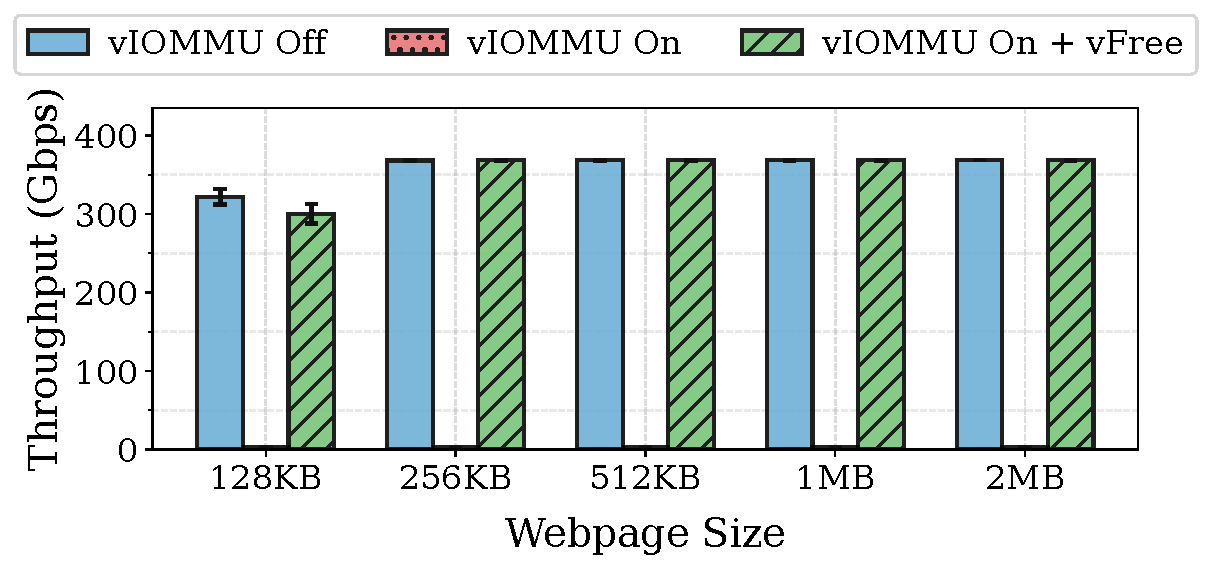
\includegraphics[width=\textwidth]{figures/nginx_size_sweep.pdf}
        \caption{NGINX}
        \label{vfree:fig:nginx}
    \end{subfigure}
    \hfill
    \begin{subfigure}[b]{0.32\textwidth}
        \centering
        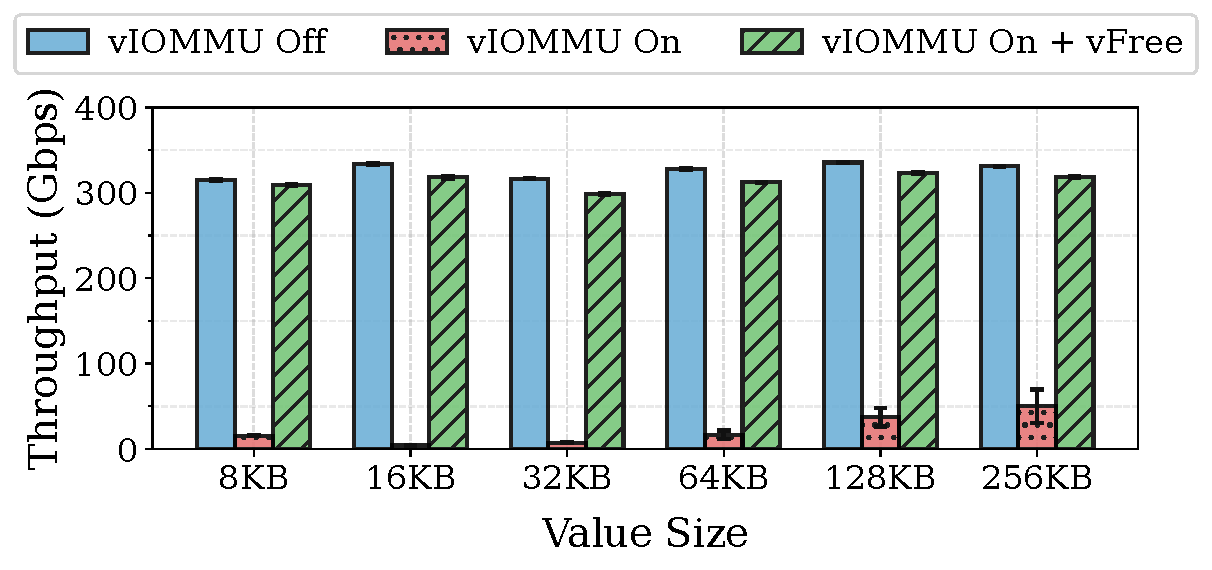
\includegraphics[width=\textwidth]{figures/redis_value_sweep.pdf}
        \caption{Redis}
        \label{vfree:fig:redis}
    \end{subfigure}
    \hfill
    \begin{subfigure}[b]{0.32\textwidth}
        \centering
        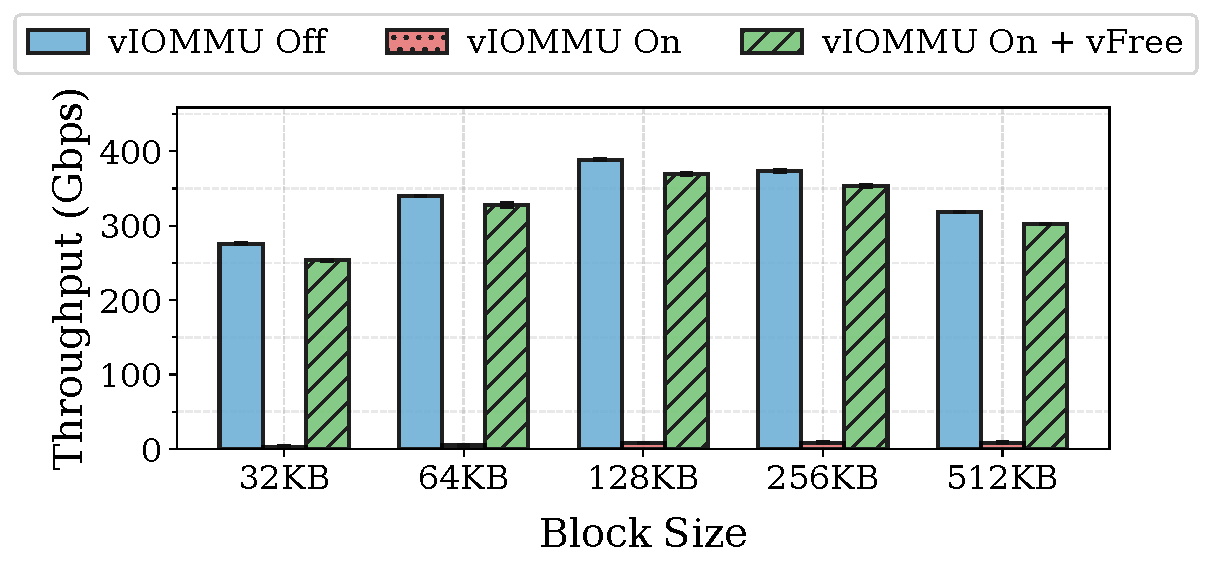
\includegraphics[width=\textwidth]{figures/spdk_fio_block_sizes.pdf}
        \caption{SPDK}
        \label{vfree:fig:spdk}
    \end{subfigure}
    \caption{\small {\bf \vfreebrand enables high-performance networked applications to
        achieve close-to-vIOMMU-off performance with strict protection, 
        consistently delivering low overhead across all evaluated applications.}}
    % Performance of real-world applications across receiver, transmitter, and mixed traffic workloads. 
    % Enabling vIOMMU causes up to 99\% throughput degradation. \vfreebrand delivers close-to-vIOMMU-off performance, with at most an 8\% throughput gap.
    \label{vfree:fig:apps}
\end{figure}


\subsubsection{Code Optimizations}
\label{vfree:sec:other-opt}

% \tianyin{reviewers may ask you how much these optimizations count in your evaluation}

{\bf Reducing critical sections.}
With nested translation,
    invalidation is only required for unmap operations, not map operations~\cite{intel_vtd_spec}.
However, vanilla Linux acquires the per-IO-domain lock at map time
    to check if the domain uses nested translation and if a write-buffer flush is needed for legacy devices.
The implementation is inefficient as both can be determined at domain creation time.
% If neither condition applies, the kernel releases the lock without performing any operation.
% Because the same lock is contended during unmap-side invalidation (\S\ref{vfree:sec:inefficiencies}),
% this unnecessary acquisition at map time exacerbates lock contention.
% We observe that both conditions---first-stage translation mode and write-buffer flush requirement---are
% determined at domain creation time and never change afterward.
\vfreebrand precomputes these attributes and skips the lock acquisition at map time.
% This optimization is general and can be applied to the vanilla kernel as well.

\para{Leveraging IOVA contiguity.}
Inspired by prior work~\cite{Rubin2024FastSafe},
we leverage IOVA contiguity to reduce the number of \CodeIn{map} and \CodeIn{unmap()} calls on the mlx5 Tx path.
Each socket buffer may contain multiple fragments of physically discontinuous pages.
In the vanilla driver, each fragment is mapped and unmapped individually.
We instead use the scatterlist DMA API to map all fragments into a single contiguous IOVA range
and unmap them in a single call, reducing the number of invalidation requests
generated from \CodeIn{unmap()} operations. % (less than 200~LOC).

% Again, the receiver path is optimized with page pool optimization, so the technique is no longer neccessary.



\if 0 % this is too fine-grained
\subsubsection{Runtime Configurability}
Both optimizations are independently controlled via kernel command-line parameters: \texttt{intel\_iommu\_pinned=on|off} selects between the pinned and distributed flush strategies, and
\texttt{intel\_iommu\_dfp=on|off} enables or disables Deferred Page Free.
The maximum number of flush iterations per leader invocation is exposed as a runtime-tunable parameter via \texttt{debugfs}, allowing adjustment without kernel recompilation.
\fi 




\subsection{Evaluation}
\label{vfree:sec:eval}


This section presents {\vfreename} evaluation. We first discuss {\vfreename} benefits for three real-world applications (\S\ref{vfree:ssec:real-world}), and then dive deeper into understanding {\vfreename} benefits using microbenchmarks (\S\ref{vfree:ssec:micro}). Next, we perform an ablation study of {\vfreename} design ideas (\S\ref{vfree:ssec:ablation}), discuss {\vfreename} scalability with increasing number of VMs (\S\ref{vfree:sec:eval-multi-vm}), and finally also discuss any associated costs of using {\vfreename} (\S\ref{vfree:ssec:cost}). 
% compared with vanilla system with vIOMMU on and off. 
% We use the pinned consumer configuration of {\vfreename}.
Unless stated otherwise, the system setup is the same as described in \S\ref{vfree:sec:inefficiencies}. 
% \saksham{Comback here to add overview}

\para{Measurement setups.}
% \schaic{All comments resolved. @Rachit please check.}
As mentioned in \S\ref{vfree:sec:inefficiencies}, we use two servers with Emerald Rapids processor architecture (which supports nested translation) directly connected to each other via $400$Gbps Nvidia ConnectX-7 NICs; this is to ensure that performance bottlenecks are not in the network. 
% The servers have  
%   with Intel Xeon Platinum 8592V CPUs and Intel Xeon Gold 6538Y+ CPUs respectively. 
% The former hosts our VMs, 
%   and the latter acts as client to send or receive traffic to the VM. 
  % a passive server engaged in Rx or Tx traffic 
  % \rachit{we have to be careful: each server does both Rx and Tx---right?}.  
% Each server has an Nvidia ConnectX-7 NIC; the two NICs connected to Ethernet with 400Gbps access link bandwidth.
These servers are 4-socket servers; each socket has
  32 physical cores, 252GB of memory and 150GB/s of memory bandwidth.
  % per-socket. 
The host server, guest VM, and client machines run with Ubuntu 22.04 and Linux v6.12.9. 
% \saksham{KVM/QEMU versions?} 
The VMs are hosted by QEMU v10.0 with nested translation~\cite{yiliu1765qemu}
and unmodified host OS (Linux 6.12.9).
% \saksham{Static pinning of vCPUs to physical cores to avoid interference.} 
We place the VMs on the NIC-local NUMA node to avoid any interference/degradation 
  due to cross-NUMA traffic.
Every vCPU of the VM is pinned to a separate physical core on the host to avoid interference. 
  We disable hyperthreading, CPU frequency scaling (we fix cores at their base frequency), and NUMA balancing for stable performance. 
Unless otherwise specified, we run all VMs with 32 vCPUs.
% We built a ebpf-based tool to measure the performance of guest and host OS.
% \saksham{if we get time, we should add error bars with stddev}.
% \schaic{We already have errors bars in the latest version @Saksham.}

We use Iperf3~\cite{iperf3} to generate network traffic and measure throughput.
We measure CPU utilization with sar~\cite{sar}.
We use eBPF probes to record the execution time and invocation counts of relevant kernel functions.
We measure VM exit counts, reasons, and time with perf~\cite{perf}.
We enable TCP Segmentation Offload (TSO), Generic Receive Offload (GRO), and adaptive Receive Flow Steering (aRFS)
to reflect high-performance networks. We run each experiment five times, and present the average results and standard deviation.



% We run the VM as receiver (Rx) 
%   and trasmitter (Tx) 
%   of network traffic, respectively, in two sets of experiments; this helps us isolate the impact of I/O memory protection on each setup. \rachit{this continues to be very confusing---saying that VM is the receiver of network traffic is incorrect since it also does Tx. We should precisely define what these two setups are: Rx receives large payloads and transmits ACKs; Tx transmits large payloads and receives ACKs;}
% Tx and Rx cases separately to isolate the impact of I/O memory protection on each datapath
%   (full-system results in \S\ref{vfree:sec:eval}). 
  % \rachit{readers may find this confusing---each server does both Rx and Tx.}
% later in eval section we run an end-to-end scenario where both kinds of traffic are running concurrently.
% \schai{: receive (Figure~\ref{vfree:fig:motivation-rx}) and transmit (Figure~\ref{vfree:fig:motivation-tx}).
% \noindent
% We increase the number of flows (each pinned to a core in the VM)
%   and compare throughput when running with
%   (1) vIOMMU off and (2) vIOMMU with strict memory protection (using nested translation).
% This section presents minimalist results to build an in-depth understanding of inefficiencies in strict intra-guest IO memory protection;
%   full results, including those for real-world applications, are 
%   in \S\ref{vfree:sec:eval}.


% \saksham{Let's not use the word nested in eval; we have already established earlier that we assume nested in this paper.}
% \saksham{we shouldn;t even use it in plots, draws unnecesary attention to nested vs shadow}

% We begin with real-world applications to highlight as much as $99\%$ throughput degradation with vIOMMU On.
% \saksham{let's not use such adjectives in papers :-); we just present the results and leave to the readers to infer its abysmal. we can simply say xyz percent degradation}
% \ikdelete{ and remarkable}
% \saksham{same comment as above for the word remarkable}
% \ikdelete{ improvements provided by \vfreename}
% With \name, we closely match the vIOMMU Off performance.
% We then analyze microbenchmark results for both Rx and Tx traffic to better understand the sources of degradation and how \vfreename mitigates them.
% Finally, we examine how each component of \vfreename\ contributes to overall performance, 
% as well as its resource overhead and the effect of key design choices.

\subsubsection{{\vfreename} Benefits for Real-world Applications}
\label{vfree:ssec:real-world}
We show the benefits of using {\vfreename} for three widely used high-performance 
    networked applications: 
    NGINX (a web server), 
    Redis (a distributed key-value store), 
    and SPDK (a userspace storage stack that uses Linux TCP stack for remote storage).
We use the same setup as earlier along with $9$KB MTU size. This helps maximize the application performance and avoid CPU becoming the performance bottleneck, when running with vIOMMU off. This allows us to focus mainly on IO memory protection-induced overheads when enabling vIOMMU and/or {\vfreename}. 
% To utilize the 400Gbps link bandwidth, we use 24 cores and a 9K MTU size~\cite{Rubin2024FastSafe}.
We use similar workloads for these applications as in prior work~\cite{Rubin2024FastSafe}; we describe them below inline with each application.  The NGINX workload most closely resembles the Tx-server setup, Redis to Rx-server setup, and SPDK has characteristics of both. 
% enabling a robust evaluation of {\vfreename} across traffic patterns.
% \schaic{@Saksham, I don't think Rx-host and Tx-host are standard terminology. 
% I changed to runs as receiver, transmitter, and concurrent receiver and transmitter.}
% \saksham{We should define the terminology in S3, and stick with it; I think a better terminology would be "Rx-host", "Tx-host" and host with concurrent Rx and Tx traffic}\ik{following the suggested terminology}.

\para{NGINX.} % Using nginx, we test \name's ability to handle Tx traffic.
% \saksham{we need to say why? give intuition that servers have majority Tx traffic because they serve HTTP GET requests from clients}. 
We run an NGINX instance inside a VM (which auto-scales to increasing load by spawning more worker threads). 
On the other host, we launch 24 clients, each pinned to a separate core. 
The clients use the \texttt{wrk} benchmark~\cite{wrk} to issue HTTP \texttt{GET} requests to the server.
We vary sizes of the requested webpage from 128 KB to 2 MB and report the aggregate throughput for each webpage size.

Figure~\ref{vfree:fig:nginx} shows over {$99\%$} throughput degradation with vIOMMU-on, 
    consistently across all evaluated webpage sizes.
\vfreebrand improves throughput by up to 147$\times$ over vIOMMU-on,
    and achieves close-to-vIOMMU-off performance for webpage sizes of 256\,KB and above, and within 7\% for 128\,KB.

% The gap at 128\,KB is due to smaller webpages causing more IO transactions per byte, 
%     increasing the number of unmap and invalidation requests vFree has to handle per unit of time. 
    
    % \ik{The simplest way to explain this is using CPU bottleneck. 128kB is already bottlenecked at vIOMMU off; lets say vFree has some extra CPU overhead => some degradation over vIOMMU off performance}


% \saksham{again, let's not use subjective terms---a value may be par for some and subpar for some :-). Just provide the results and let people infer.} 
% nginx Tx\saksham{no need to repeat "Tx" again} performance with vIOMMU on. 
% The throughput degradation is consistent across all webpage sizes, with over $99\%$ throughput degradation
% \saksham{same feedback as earlier for times vs percentage}\ikdelete{. This degradation is consistent across all webpage sizes}\saksham{repeated statement}. 

% Figure~\ref{vfree:fig:nginx} exhibits subpar
% \saksham{again, let's not use subjective terms---a value may be par for some and subpar for some :-). Just provide the results and let people infer.} 
% nginx Tx\saksham{no need to repeat "Tx" again} performance with vIOMMU on. 
% The throughput degradation is consistent across all webpage sizes, with over $99\%$ throughput degradation
% \saksham{same feedback as earlier for times vs percentage}\ikdelete{. This degradation is consistent across all webpage sizes}\saksham{repeated statement}. 
% Using {\vfreename}, the throughput is restored to near-vIOMMU-off performance\saksham{instead of phrases like throughput is restored, use simpler to-the-point phrases, like \vfreename provides close-to-vIOMMU-disabled performance}\ikdelete{, with strict invalidation policy enabled}\saksham{no need to repeat this again}.

\para{Redis.} 
% Using Redis, we test \name's ability to handle Rx traffic.
We run 24 Redis server instances inside a VM, with one instance per core. 
We use redis-benchmark~\cite{redis-benchmark} to launch an equal number of client instances on the other host,
    each sending \texttt{SET} requests to a corresponding server instance. 
We vary the \texttt{SET} value size from 8 KB to 256 KB, and 
    for each value size, we follow prior work~\cite{Rubin2024FastSafe} 
    to tune the number of parallel connections, client threads, and request batch size
    and report the optimal aggregated throughput.


Figure~\ref{vfree:fig:redis} shows that vIOMMU-on
% \ikdelete{ with strict protection}\saksham{we dont have to say strict protection again, just say it once during setup that you assume this, unless specified otherwise} 
can cause up to $98\%$ throughput degradation
% \saksham{I think we should use percentage degradation, instead of xyz times} 
with higher degradation for smaller \texttt{SET} value sizes (<= 64KB).
% \ikdelete{, with smaller }
% \saksham{smaller values of what?}\ikdelete{ leading to even worse performance}.
\vfreebrand improves throughput by up to 74$\times$ over vIOMMU-on 
    and achieves close-to-vIOMMU-off performance, with at most 6\% gap.



\begin{figure}[H]
    \centering
    \begin{subfigure}[b]{0.32\textwidth}
        \centering
        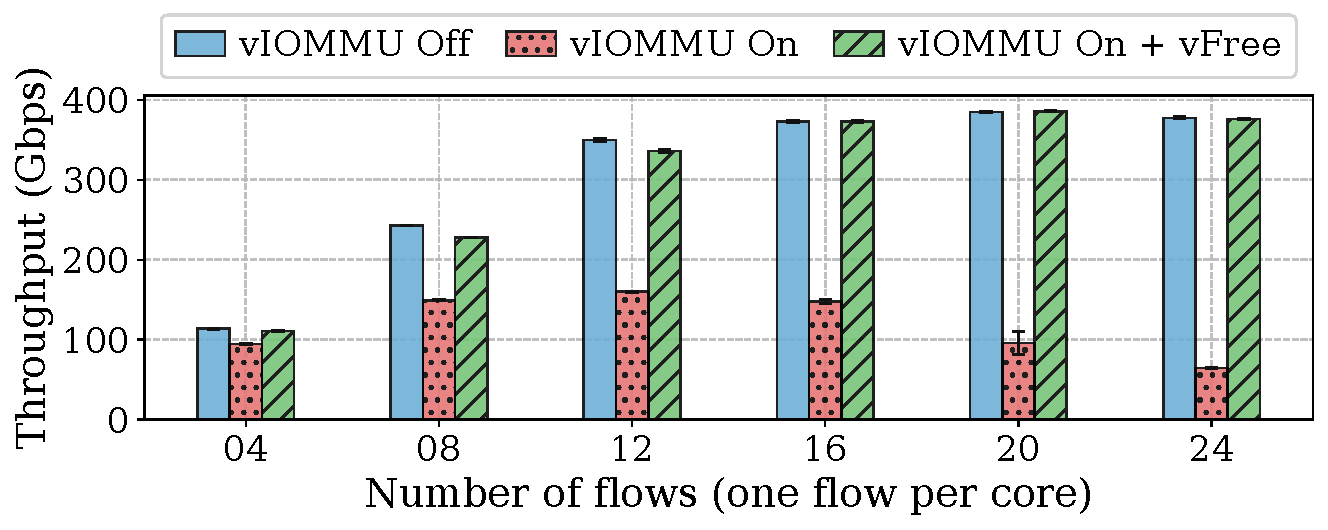
\includegraphics[width=\textwidth]{figures/eval_core_exp-tput.pdf}
        \caption{Throughput}
        \label{vfree:fig:eval-core-tput}
    \end{subfigure}
    \hfill
    \begin{subfigure}[b]{0.32\textwidth}
        \centering
        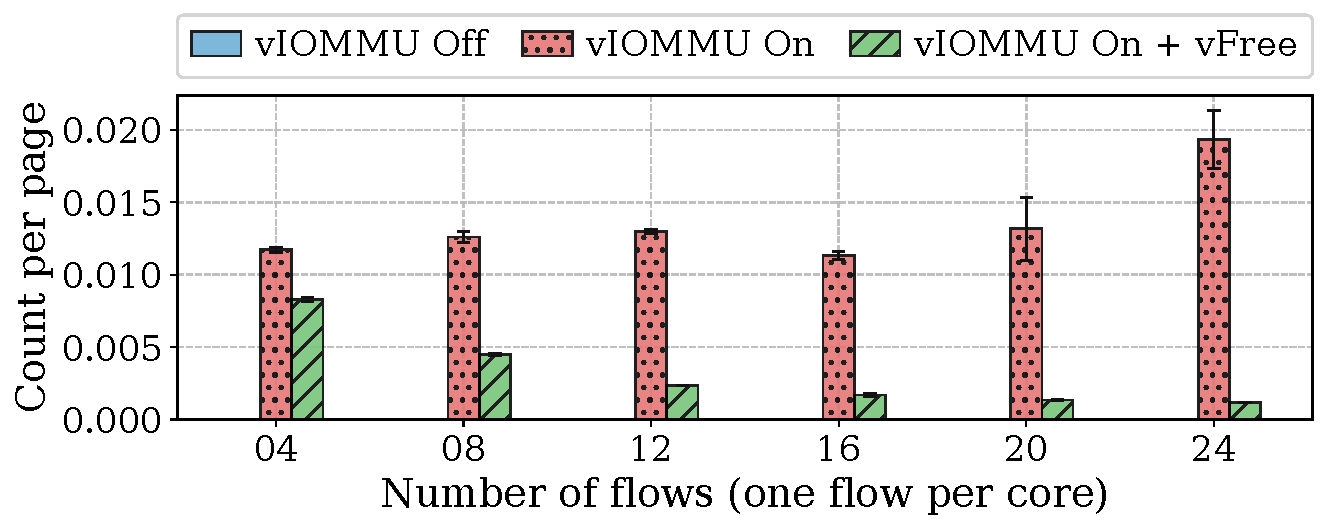
\includegraphics[width=\textwidth]{figures/eval_core_exp-qi_submit_sync-count_per_page.pdf}
        \caption{IR-SUB count per page}
        \label{vfree:fig:eval-core-qi}
    \end{subfigure}
    \hfill
    % \begin{subfigure}[b]{0.32\textwidth}
    %     \centering
    %     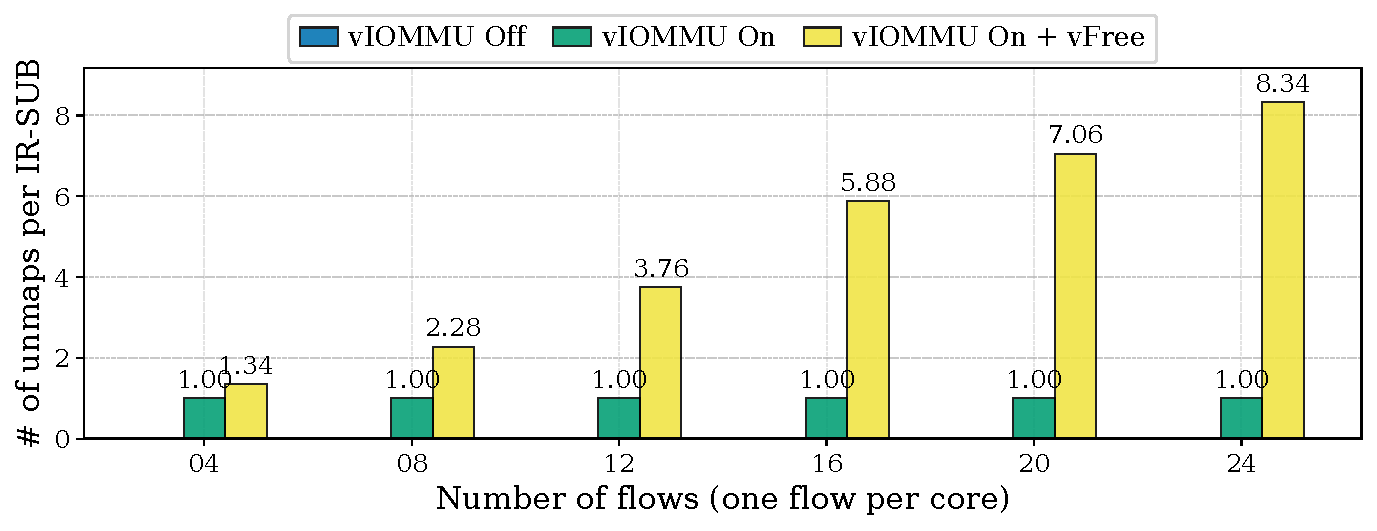
\includegraphics[width=\textwidth]{figures/eval_core_exp-unmap_to_qi_submit_ratio.pdf}
    %     \caption{Number of IR per IR-SUB}
    %     \label{vfree:fig:eval-core-unmap-ratio}
    % \end{subfigure}
    % \hfill
    \begin{subfigure}[b]{0.32\textwidth}
        \centering
        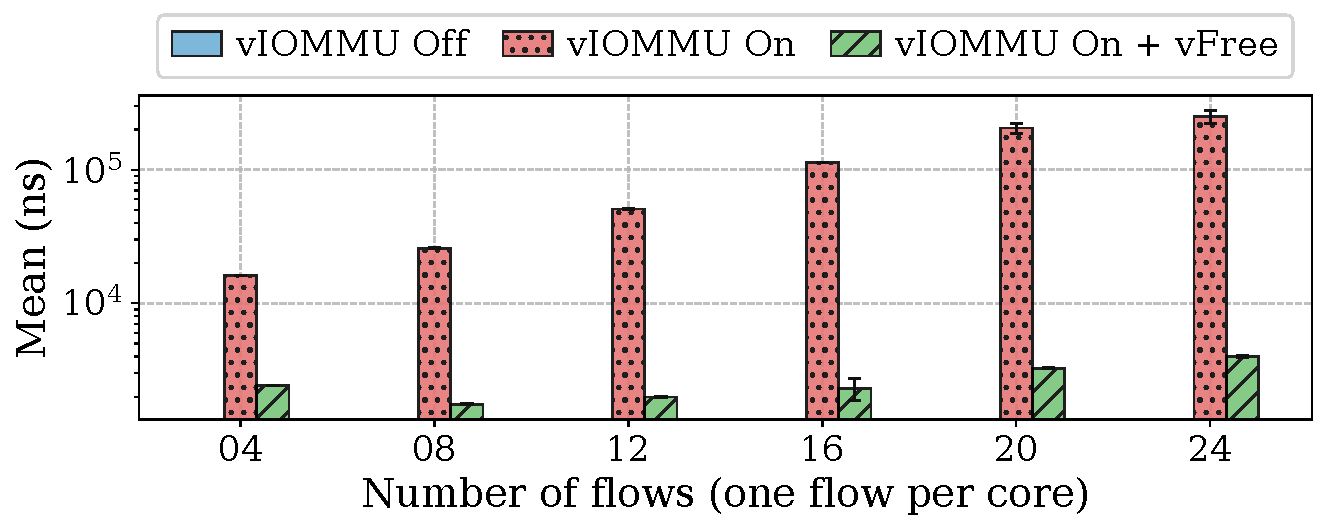
\includegraphics[width=\textwidth]{figures/eval_core_exp-cache_tag_flush_range-mean_ns.pdf}
        \caption{IR processing latency per unmap}
        \label{vfree:fig:eval-core-flush}
    \end{subfigure}
    \caption{\small {\bf Rx-server.} \vfreename{} achieves up to $4.9\times$ Rx throughput improvement over vIOMMU-on.}
%    \schaic{c)'s caption is a bit hard in one line. See text for detailed definition.}}
    \label{vfree:fig:eval-core}
\end{figure}

\begin{figure}[H]
    \centering
    \begin{subfigure}[b]{0.32\textwidth}
        \centering
        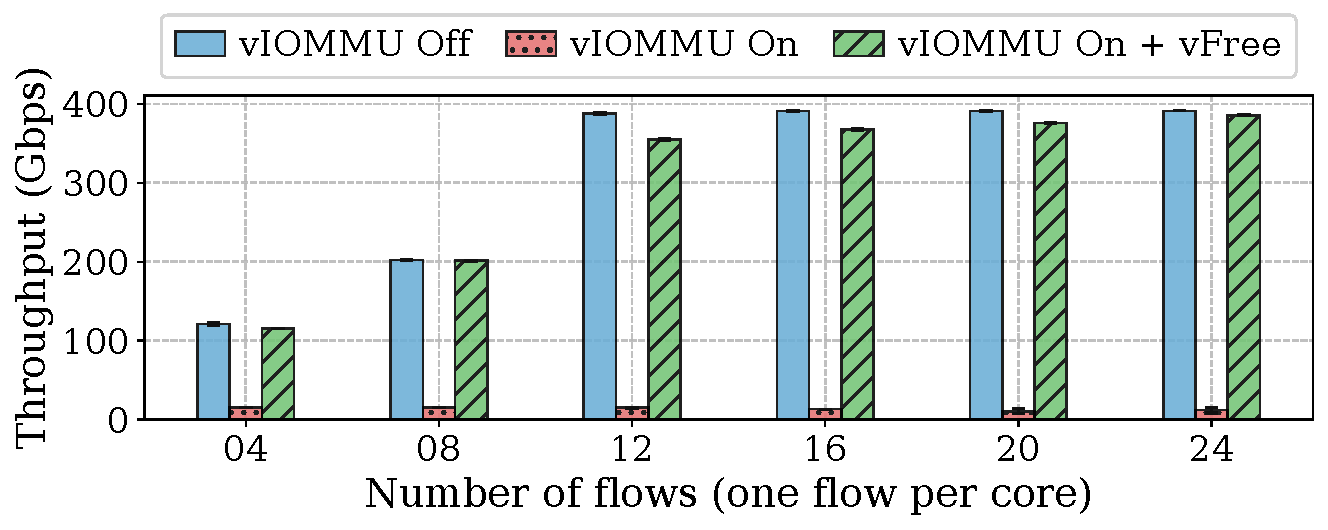
\includegraphics[width=\textwidth]{figures/tx-ebpf-tput.pdf}
        \caption{Throughput}
        \label{vfree:fig:tx-tput}
    \end{subfigure}
    \hfill
    \begin{subfigure}[b]{0.32\textwidth}
        \centering
        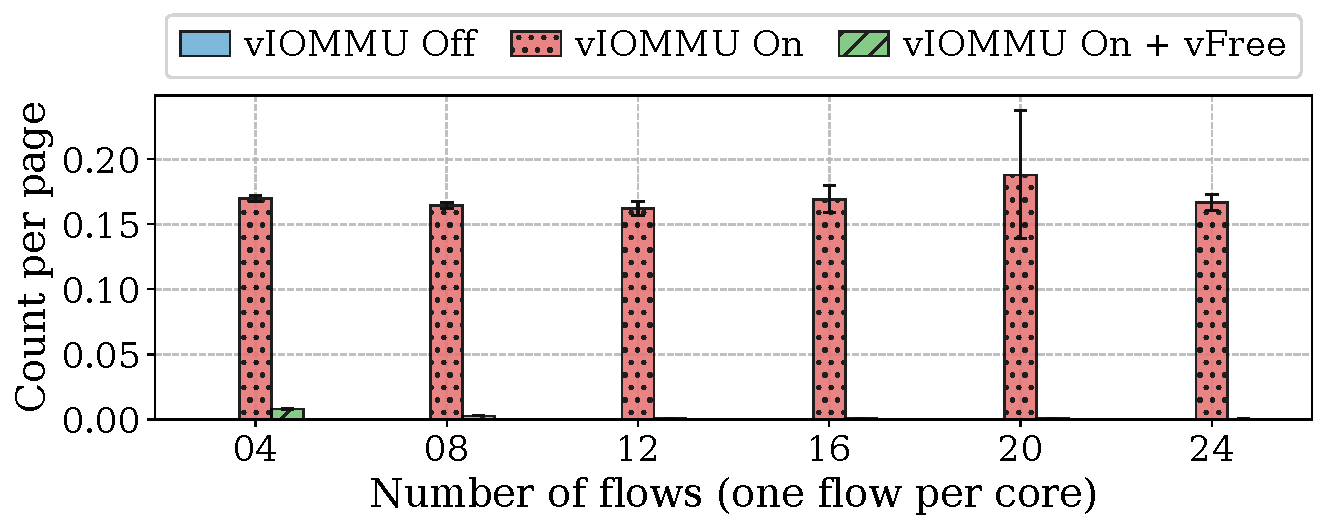
\includegraphics[width=\textwidth]{figures/tx-ebpf-qi_submit_sync-count_per_page.pdf}
        \caption{IR-SUB count per page}
        \label{vfree:fig:tx-qi}
    \end{subfigure}
    \hfill
    \begin{subfigure}[b]{0.32\textwidth}
        \centering
        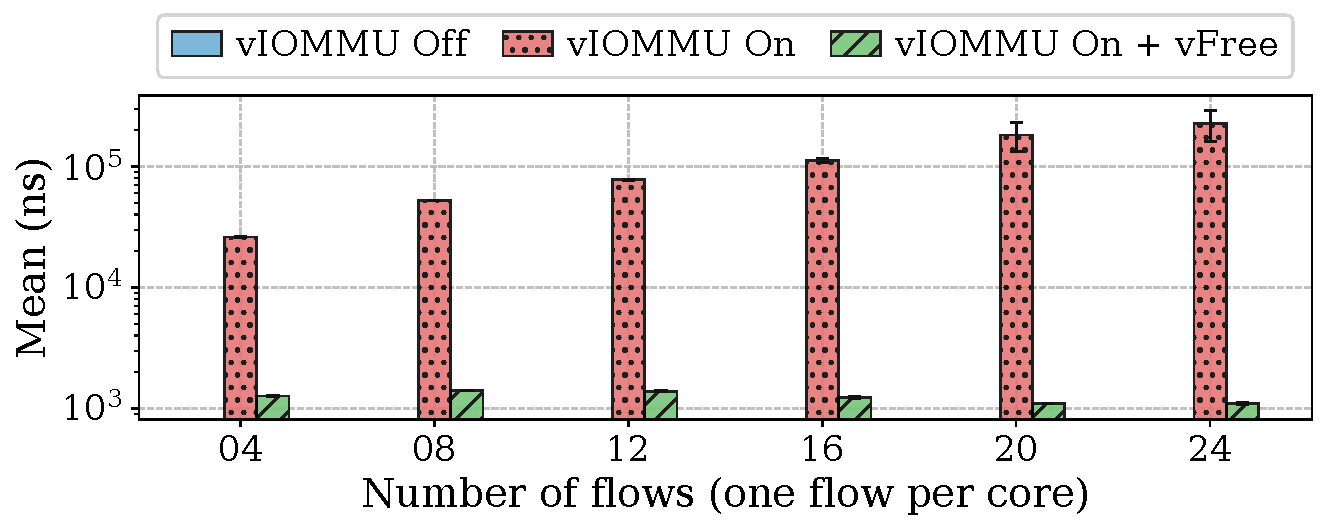
\includegraphics[width=\textwidth]{figures/tx-ebpf-cache_tag_flush_range-mean_ns.pdf}
        \caption{IR processing latency per unmap}
        \label{vfree:fig:tx-flush}
    \end{subfigure} 
%    \caption{Tx microbenchmark (one flow per core): \vfreename{} achieves up to $36\times$ throughput improvement over the vIOMMU On configuration
%    by reducing IR-SUB count per page and IOTLB invalidation overhead.
    \caption{\small {\bf Tx-server.} \vfreename{} achieves up to 36$\times$ Tx throughput improvement over vIOMMU-on.}
    \label{vfree:fig:tx}
\end{figure}

\para{SPDK.} 
% To stress-test \name's ability to handle concurrent Rx and Tx traffic,
% We configure SPDK to serve a mix of read and write IO requests over TCP.
% We use SPDK to evaluate a workload where the VM concurrently receives and transmits network traffic, 
% thereby stressing both Rx and Tx datapaths. 
We create a RAM-backed block device and run 24 SPDK server instances inside a VM, one per core.
On the other host, we run an equal number of \texttt{fio}~\cite{fio} clients, 
    each generating a workload with 60\% reads and 40\% writes and an IO depth of 8\footnote{We opt for 60:40 read-write ratio and IO depth 8 to avoid memory bandwidth bottleneck. 
    In general, writes consume twice the memory bandwidth 
    of reads, as each write involves a memory read followed by a memory write.}.
We vary the block size from 32 KB to 512 KB and report the aggregate throughput.
% \saksham{Try to give more context as to why we create so much fuss about mixed workload---that there would be more no. of unmap requests the IOMMU will have to serve?}\ik{We do not have a good reason besides stressing both Rx and Tx datapaths, and creating a more realistic scenario. The original plan was to use Rx (SET) only, but that lead to memory BW bottleneck.}

Figure~\ref{vfree:fig:spdk} shows over 97\% throughput degradation 
    with vIOMMU-on across all block sizes.
\vfreebrand improves throughput by up to 82$\times$ over vIOMMU-on and 
    achieves close-to-vIOMMU-Off performance, with at most an 8\% gap.

% The gap of 8\% happens at the smallest block size of 32\,KB which 
    % has more overhead (similar to small webpages in NGINX).

% \vspace{0.1in}
% \noindent
% The small, 6-8\%, performance gap is observed only for the smallest-sized IO requests in all three applications. This is because CPU became the bottleneck for these cases even for vIOMMU-off, and additional CPU cycles spent on map/unmap operations with {\vfreename} led to slightly lower throughput. 
    
% Smaller block sizes result in more IO transactions per byte, 
%    increasing the number of unmap calls and invalidation requests that vFree has to handle per unit of time.}

% \textbf{SPDK.} We use SPDK to evaluate concurrent Rx and Tx traffic\saksham{use consistent terminology defined earlier}, thereby stressing datapaths. To configure SPDK, we first create a\ikdelete{ "malloc"}\saksham{"malloc" not needed} block device (backed by RAM) to serve \ikreplace{read and write}{IO} requests over TCP\saksham{say IO requests here; later we show IO workload with read:write ratio}. We then run 24 SPDK server instances inside the VM, with one instance pinned to each core. The other host\saksham{terminology} runs an equal number of \texttt{fio} \cite{fio} clients, each generating a workload with 60\% reads and 40\% writes\saksham{why did we use 60:40? is it something standard workload, or used in prior work? Why not just 50:50?}\ik{Why not 50:50 addressed in footnote. In fact, we use a mixed workload only to avoid memory BW bottleneck}\footnote{We use a 60:40 split of reads v/s writes to avoid memory bandwidth bottleneck. Writes consume twice the memory bandwidth of reads as each write involves a memory read followed by a memory write.} at an IO depth of 8\footnote{We choose an IO depth of 8, as increasing it further does not improve throughput due to memory bandwidth bottlenecks on the SPDK server.}\saksham{why 8? is it the knee point?}. We vary the block size from 16 KB to 512 KB and report the aggregate throughput across reads and writes.
% \saksham{Try to give more context as to why we create so much fuss about mixed workload---that there would be more no. of unmap requests the IOMMU will have to serve?}\ik{We do not have a good reason besides stressing both Rx and Tx datapaths, and creating a more realistic scenario. The original plan was to use Rx (SET) only, but that lead to memory BW bottleneck.}

\subsubsection{Understanding {\vfreename} Benefits}
\label{vfree:ssec:micro}
% Section~\ref{vfree:sec:inefficiencies} presents the overhead of memory protection with vIOMMU.

To better understand the reasons for {\vfreename} performance benefits, we also evaluate {\vfreename} using microbenchmarks. We use Iperf3~\cite{iperf3} to generate network traffic and measure throughput. We use similar setup as in \S\ref{vfree:sec:inefficiencies}, running same sets of controlled experiments, with the VM acting as the Tx-server and Rx-server, respectively. This enables us to analyze the individual impact of these setups on {\vfreename} performance.



\para{Rx-server.} 
% \ikdelete{ We evaluate this setup under the three configurations described in \S\ref{vfree:sec:eval}}
% \saksham{last line is not necessary; already mentioned in setup}
% \ikdelete{. Enabling vIOMMU in strict mode significantly degrades performance compared to vIOMMU off}
% \saksham{this was already discussed earlier in S3, when discussing fig 2}
% In contrast, \vfreename restores throughput to near-vIOMMU-off level.
% \saksham{"restores"}
% \ikdelete{ while preserving the same security guarantees as strict invalidation policy}
% \saksham{this repetitive; and even then also inconsistent, sometimes it says strict protection, sometimes strict invalidation policy}
% Overall, \vfreebrand achieves up to a $83\%$ throughput improvement over the vIOMMU on configuration.
As shown in Figure~\ref{vfree:fig:eval-core-tput}, {\vfreename} improves throughput by up to $4.9\times$ in comparison to vIOMMU-on, 
matching closely to vIOMMU-off performance (with a maximum gap of <6\%).
The key contributor to this throughput improvement is the reduction of IR-SUB operations per page transferred over network. As shown in Figure~\ref{vfree:fig:eval-core-qi}, {\vfreename} reduces the IR-SUB count per page by up to 82\%. Recall from \S\ref{vfree:sec:background-datapath}, each IR-SUB operation requires an unavoidable VM exit, hence, reduction in IR-SUB count translates to a similar reduction in VM exits per page. {\vfreename} achieves this reduction using two design ideas. One-for-many invalidations allow using a single IR-SUB to invalidate concurrently prepared IRs across multiple cores---hence, we see lower IR-SUB counts per page with increasing numbers of cores in Figure~\ref{vfree:fig:eval-core-qi}. Furthermore, deferred free page allows each core to prepare multiple IRs that can be concurrently processed by a single IR-SUB operation. This is achieved by avoiding busy waiting by each core until successful invalidation for each prepared IR, and hence reducing the time spent on IR processing by the core after {\tt unmap}. Figure~\ref{vfree:fig:eval-core-flush} shows the average time spent by application core on IR processing: while vIOMMU-on incurs large IR processing time due to incurring all---\CodeIn{cache\_lock} contention, IR-PREP and IR-SUB overheads,  {\vfreename} avoids lock contention due to its per-CPU locks, and avoids IR-SUB due to deferred free page, and observes up to 99.9\% reduction in IR processing time. 

\para{Tx-server.} 
Figure~\ref{vfree:fig:tx-tput} shows that {\vfreename} achieves up to 36$\times$ throughput improvement over vIOMMU-on,
closely matching vIOMMU-off (with the largest gap of <9\%). The root cause of {\vfreename} benefits are similar to those discussed earlier for the Rx-server case. We briefly discuss the reason behind the relatively larger throughput gains in the Tx-server case. This is because of larger number of unmaps per page performed in Tx datapath (recall that Linux's page pool optimization does not apply to Tx datapath; \S\ref{vfree:sec:background-datapath}). Due to much larger number of unmaps per page, {\vfreename} is able to enqueue much larger number of IR descriptors into the IO-domain queue, which can be submitted using a single IR-SUB---hence further reducing the IR-SUB count per page (as evident from Figure~\ref{vfree:fig:tx-qi}). This leads to relatively larger reductions in VM exits per page for Tx-server case, improving the relative performance gains.

% Both \optOne{} and DFP contribute significantly to the improvements\ik{but in ablation we say DFP is the primary; which is accurate; would be good to mention somewhere that primary contributors to performance are different in Tx and Rx}.
% \optOne{} aggregates multiple invalidation requests into a single IR-SUB operation,
% reducing the IR-SUB count per page by $300\times$ (Figure~\ref{vfree:fig:tx-qi}).
% DFP further increases the batching factor by releasing producer threads from waiting for invalidation to complete,
% reducing the average time the guest spends in the IOMMU subsystem by over 200$\times$ (Figure~\ref{vfree:fig:tx-flush}).


% With vanilla Linux and mlx5 driver, every transmitted socket buffer triggers at least one map, 
%     one unmap, and one cache invalidation---exerting
%     high pressure on the IOMMU subsystem and resulting in a 15$\times$ 
%     higher IR-SUB count per page compared to the Rx case (Figure~\ref{vfree:fig:tx-qi}).

% \schaic{Consider Removing fig:stress-qi and fig:stress-flush if we are short of space.}


% Rather than stalling on each invalidation, producer threads enqueue their requests and continue execution.

% Reduction by by up to 99.9\%
% the near-total reduction confirms that {\vfreename} effectively eliminates both bottlenecks.

% through \optOne{}---which aggregates multiple invalidation requests into a single IR-SUB operation. 


% This batching scales with parallelism: the number of invalidation requests handled per IR-SUB grows linearly from 1.3 to 8.3 as the number of active cores increases.

% DFP further enables asynchronous invalidation without losing strict safety guarantees.


% As shown in Figure~\ref{vfree:fig:eval-core-flush}, {\vfreename} reduces the average time the guest OS spends in the IOMMU subsystem for IOTLB invalidation by up to 99.9\%,
% almost completely eliminating invalidation overhead.
% This metric subsumes locking contention and IR-SUB operation in Figure~\ref{vfree:fig:lock-contention};
% the near-total reduction confirms that {\vfreename} effectively eliminates both bottlenecks.

% \ik{does not match with ablation study data where we say atmost 3 in a batch; it is important to clarify that these numbers are with DFP which can increase batch size} 

% In this experiment, the VM acts as receiver while the client serves as sender.
% \ikdelete{ We evaluate this setup under the three configurations described in \S\ref{vfree:sec:eval}}\saksham{last line is not necessary; already mentioned in setup}\ikdelete{. Enabling vIOMMU in strict mode significantly degrades performance compared to vIOMMU off}\saksham{this was already discussed earlier in S3, when discussing fig 2} In contrast, \vfreebrand restores\saksham{"restores"} throughput to near-vIOMMU-off level\ikdelete{ while preserving the same security guarantees as strict invalidation policy}\saksham{this repetitive; and even then also inconsistent, sometimes it says strict protection, sometimes strict invalidation policy}. Overall, \vfreebrand achieves up to a $83\%$ throughput improvement over the vIOMMU on configuration.

% A key factor behind the substantial throughput improvement is the reduction in VM exits, due to fewer invalidation requests. As shown in Figure~\ref{vfree:fig:eval-core-qi}, \vfreebrand lowers invalidations per page by up to $82\%$ through delegated invalidation: requests from multiple cores are aggregated, and a single core issues a batched invalidation request. Importantly, a batched invalidation to the IOMMU hardware takes roughly the same time as an individual request, so the duration of each VM exit remains unchanged. Another contributing factor is the reduction in the total time the guest OS spends in the IOMMU subsystem, enabled by the deferred free page (DFP) optimization. During a VM exit, only the issuing core is blocked while waiting for the invalidation to complete, whereas other cores can simply enqueue their invalidation requests and continue execution without stalling. As shown in Figure~\ref{vfree:fig:eval-core-flush}, \vfreebrand reduces the average time that guests OS spends in the IOMMU subsystem by up to $99.9\%$, nearly eliminating the overhead of IOTLB invalidation.

% In Figure~\ref{vfree:fig:stress}, we stress-test \vfreebrand by varying the number of flows per core on a 24-core configuration. Combining results from Figure~\ref{vfree:fig:eval-core} and Figure~\ref{vfree:fig:stress}, we observe that \vfreebrand scales well with both increasing core counts and higher number of per-core flows. Across all scenarios, \vfreebrand closely matches vIOMMU off performance.

% A key factor behind the substantial throughput improvement is the reduction in VM exits, due to fewer invalidation requests.

% text on count per page.
% A key factor behind the substantial throughput improvement is the reduction in VM exits, due to fewer invalidation requests. 
% As shown in Figure~\ref{vfree:fig:eval-core-qi}, \vfreebrand lowers invalidations per page by up to $82\%$ through delegated invalidation:
%  requests from multiple cores are aggregated, and a single core issues a batched invalidation request. 
%  Importantly, a batched invalidation to the IOMMU hardware takes roughly the same time as an individual request, so the duration of each VM exit remains unchanged. Another contributing factor is the reduction in the total time the guest OS spends in the IOMMU subsystem, enabled by the deferred free page (DFP) optimization. During a VM exit, only the issuing core is blocked while waiting for the invalidation to complete, whereas other cores can simply enqueue their invalidation requests and continue execution without stalling. As shown in Figure~\ref{vfree:fig:eval-core-flush}, \vfreebrand reduces the average time that guests OS spends in the IOMMU subsystem by up to $99.9\%$, nearly eliminating the overhead of IOTLB invalidation.



% \schaic{I have a figure for this (eval\_core\_exp-unmap\_to\_qi\_submit\_ratio.pdf). Shall we replace it with current Figure~\ref{vfree:fig:eval-core-qi}?}

% Such "one-for-many" optimization completely changes the story of IR-PREP and IR-SUB serlization 
    % in vanilla vIOMMU on.

% aggregating multiple invalidation requests into a single IR-SUB operation.
% As we discussed in \S\ref{vfree:sec:inefficiencies},
% vIOMMU on incurs significant overhead because it couples IR-PREP and IR-SUB operations,
% and serializes them across all network threads.
% A key factor behind the substantial throughput improvement is the reduction 
% in IR-SUB operation per page.
% in VM exits, due to fewer invalidation requests. 
% As shown in Figure~\ref{vfree:fig:eval-core-unmap-ratio}, 
% vIOMMU performs one IR-SUB operation for each unmap call which corresponds to one IR.
% the cross-thread serialization of IR-PREP and IR-SUB operations in 
% \vfreename lowers invalidations per page by up to $82\%$ through delegated invalidation: 
% invalidation requests from multiple producer threads are aggregated, 
% and a single consumer thread issues one IR-SUB operation tha handles all the aggregated requests. 
% Importantly, a batched invalidation to the IOMMU hardware takes roughly the same time as an individual request, 
% so the duration of each VM exit remains unchanged. 


\if 0
We further stress-test \vfreename{} by scaling up to eight concurrent flows across 24 cores (see Figure~\ref{vfree:fig:stress}
    in the appendix).
Under excessive loads, \vfreename{} maintains throughput within 1\% of vIOMMU-off performance.
Combining the results from Figures~\ref{vfree:fig:eval-core} and~\ref{vfree:fig:stress}, 
we observe that \vfreename{} scales robustly with both increasing core counts and flows per core. 
\fi

% reduces the number of invalidation requests by over $300\times$ (Figure~\ref{vfree:fig:tx-flush}) through batching. 

% Combined with DFP, it also reduces the time the guest OS spends in the IOMMU subsystem by over $200\times$ (Figure~\ref{vfree:fig:tx-qi}), as cores can simply enqueue invalidation requests and avoid waiting for IOTLB invalidation to complete.


% \textbf{\vfreename\ performance with Tx traffic.} We use the same setup as in \S\ref{vfree:sec:inefficiencies}. 
% In this experiment, the VM acts as sender and the client as receiver, with traffic generated using Iperf.
% Figure~\ref{vfree:fig:tx} evaluates the setup under the same three configurations as described in \S\ref{vfree:sec:eval}. 


% This is because the vIOMMU on configuration incurs a much higher number of invalidations per page for Tx traffic (Figure~\ref{vfree:fig:tx-qi}) than for Rx traffic (Figure~\ref{vfree:fig:eval-core-qi}). The increase is driven by more frequent \CodeIn{map()}/\CodeIn{unmap()} operations, as discussed in \S\ref{vfree:sec:linux-opt}, leading to more VM exits and greater time per core spent waiting on the \CodeIn{cache\_lock}.

% As shown in Figure~\ref{vfree:fig:tx-tput}, the throughput degradation between vIOMMU Off and the vIOMMU On configuration is significantly more pronounced in the Tx case. Despite this, \vfreename restores throughput to near-vIOMMU-Off level. In fact, \vfreename achieves up to $98\%$ throughput improvement over the vIOMMU On configuration. Similar to the Rx case, this improvement originates from two key optimizations---delegated invalidation and DFP optimization. Delegated invalidation reduces the number of invalidation requests by over $300\times$ (Figure~\ref{vfree:fig:tx-flush}) through batching. Combined with DFP, it also reduces the time the guest OS spends in the IOMMU subsystem by over $200\times$ (Figure~\ref{vfree:fig:tx-qi}), as cores can simply enqueue invalidation requests and avoid waiting for IOTLB invalidation to complete.


\subsubsection{{\vfreename} Ablation Study}
\label{vfree:ssec:ablation}

We quantify the contributions of 
\optOne{}, deferred free page,
and other {\vfreename} code optimizations (\S\ref{vfree:sec:other-opt}) to overall throughput for both Rx- and Tx-server setups.
In our analysis, we vary the number of cores from 4 to 24, 
    each running one flow, and report the corresponding throughput.

\para{Tx-server.} Figure~\ref{vfree:fig:ablation-tx} shows that code optimizations provide a modest contribution in overall gains. One-for-many invalidations improve the throughput further by {1.1-2.9$\times$}, with increasing gains with larger core count. This is expected since more cores enable {\vfreename} to invalidate more concurrent IRs via single IR-SUB. Deferred free page, however, provides most significant contribution to throughput gains---{2.9 to 5.6$\times$}. Without deferred free page, each core stays blocked after IR-PREP until successful invalidation completion for the IR. When no longer constrained to busy wait with deferred free page, each core can continue execution of the future unmaps. And since in Tx-server setup, as discussed earlier, there are a large number of unmaps generated per core, this unblocking of cores results in significant throughput gains. 




% DFP is the primary contributor to throughput gains for Tx traffic.
% As discussed in \S\ref{vfree:sec:linux-opt},
% the Tx datapath invokes significantly more \CodeIn{map()}/\CodeIn{unmap} operations,
% resulting in a much higher rate of invalidation requests.
% While \optOne{} reduces the number of VM exits by batching these invalidations,
% it stalls threads that generate invalidation requests until its invalidation is completed (to mantain strict safety guarantee).
% % it creates a bottleneck:
% % all cores that contribute requests to a batch must synchronously wait for the invalidation to complete.
% As a result, \optOne{} alone fails to scale throughput with increasing core count.
% Although batching opportunities improve with more cores,
%     the wait for invalidation caps the throughput to the rate of IR-SUB operations.\ik{we can probably start by saying that one-to-many alone is not sufficient due to large batch sizes and more cores blocked, and then we say that DFP removes waiting so performance improves}

\para{Rx-server.} 
Unlike Tx-server, Figure~\ref{vfree:fig:ablation-rx} shows that for Rx-server, one-for-many invalidations provides more significant contribution to overall gains. This is due to relatively lower numbers of unmaps per page observed in the Rx-datapath: there is relatively smaller performance impact of unblocking the cores using deferred free page due to larger inter-arrival times between unmap requests within each core. 


% Different from Tx, both \optOne{} and DFP 
%     contribute significantly to the performance improvements 
%     over vIOMMU-on by reducing the number of VM exits. 
% % Since each invalidation triggers a VM exit, 
% % aggregating multiple invalidation requests into a single IR-SUB operation significantly lowers the overall VM exit overhead.
% Specifically, \optOne{} opportunities naturally increase with core count, 
%     improving throughput by 1.5$\times$ at 12 cores and up to 4.8$\times$ at 24 cores.
% Applying DFP atop \optOne{} yields additional gains.
% The relatively modest improvement is expected\ik{imo we see modest gains only because there is no scope to improve on top of vIOMMU off, so DFP simply fills the gap}: at high Rx traffic rates, 
%     few unmap operations---and thus few invalidation requests---are generated.
% In our profiling, 99.9+\% of IOMMU operations are generated by the Tx datapath, which primarily sends ACKs to the sender.
% % , thanks to the page pool optimization (\S\ref{vfree:sec:linux-opt}).
% With a low invalidation rate, only a small number of cores are blocked at a time, waiting for invalidation to complete.\ik{the fact that "one-to-many invalidations achieve good improvement due to small batch sizes and fewer cores blocked" is not clearly conveyed here}
% \if 0 % save space
% Consequently, \optOne{} alone achieves 71\% of vIOMMU Off performance at 12 cores and 99\% at 24 cores.
% DFP closes the residual gap by deferring page reclamation, 
% allowing even those few blocked cores to enqueue their requests and continue without stalling.
% \fi 
% % ---but the additional benefit is inherently limited when synchronization pressure is already low.


% \textbf{Rx Ablation Study.} 
% As shown in Figure~\ref{vfree:fig:ablation-rx}, SBI mitigates a large fraction of the performance lost with vIOMMU On. This improvement stems from batching invalidation requests, which reduces the number of VM exits. Since each invalidation triggers a VM exit, amortizing them across batches significantly lowers the overall VM exit overhead. Moreover, batching opportunities naturally increase with core count. As a result, the relative benefit of SBI grows with scale, improving throughput by \textasciitilde35\% at 12 cores and up to \textasciitilde83\% at 24 cores.

% Applying DFP on top of SBI yields additional, but smaller, gains. The relatively modest improvement is expected, as SBI already addresses the primary bottleneck, while DFP serves to close the residual gap. \leshna{I agree with the first line, but not the reason, why does SBI address the primary bottleneck, a small callback of we have low number of unmap may be helpful. Basically TX and RX explanation should complement} Specifically, DFP reduces time spent in the guest IOMMU subsystem by deferring page reclamation work. During a VM exit, only the issuing core is blocked, while other cores can enqueue invalidation requests and continue execution without stalling.


\begin{figure}[H]
    \centering
    \begin{subfigure}[b]{\columnwidth}
        \centering
        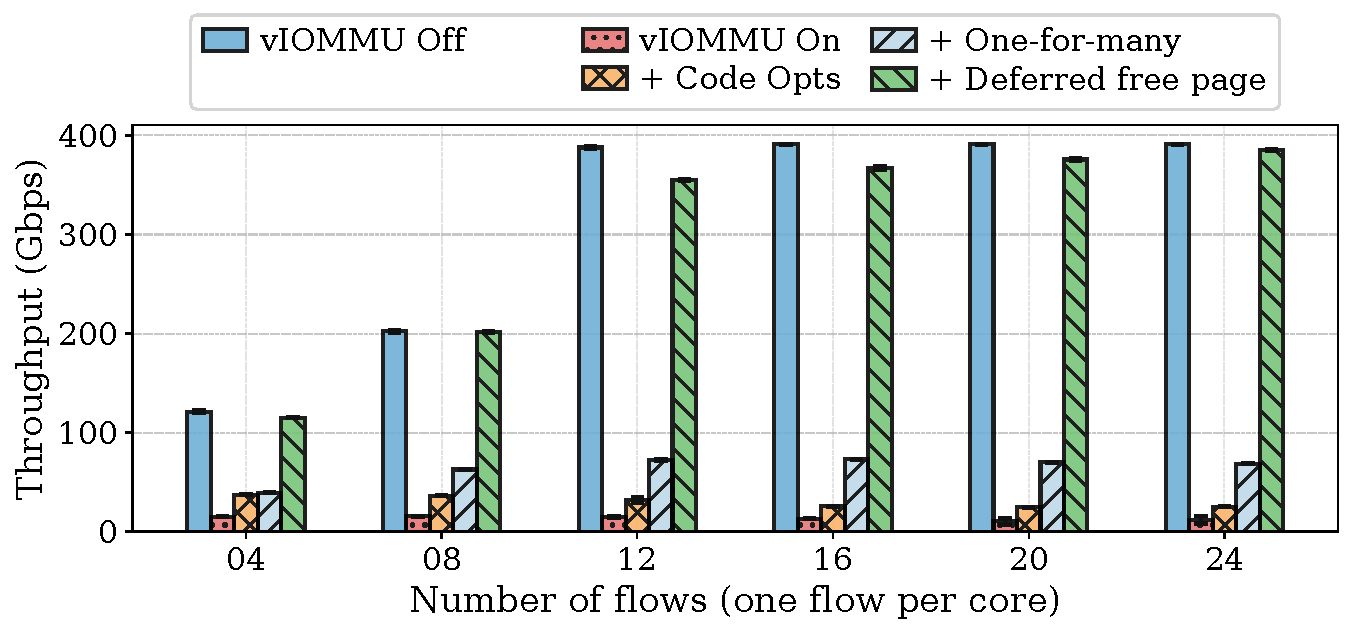
\includegraphics[width=0.95\textwidth]{figures/eval_ablation_tx-tput.pdf}
        \caption{Tx-server}
        \label{vfree:fig:ablation-tx}
    \end{subfigure}
    \begin{subfigure}[b]{\columnwidth}
        \centering
        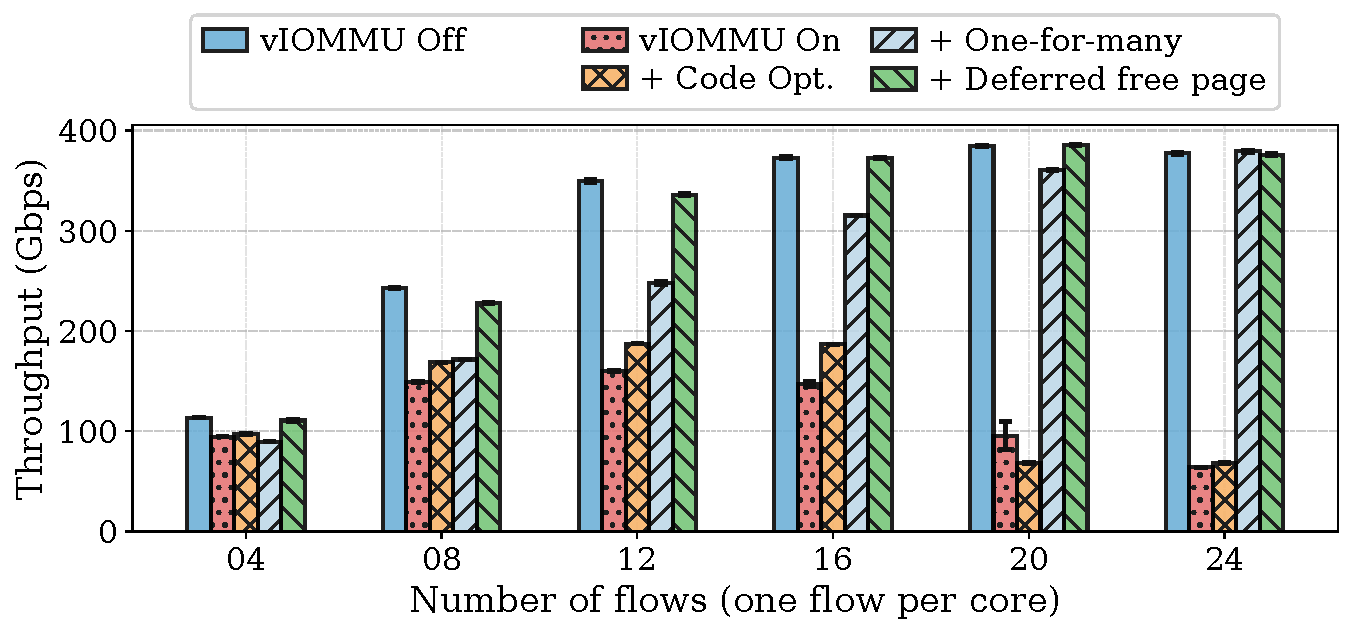
\includegraphics[width=0.95\textwidth]{figures/eval_ablation_rx-tput.pdf}
        \caption{Rx-server}
        \label{vfree:fig:ablation-rx}
    \end{subfigure}
    \caption{\small {\bf Necessity of both design ideas---one-for-many invalidations and deferred free page---to achieve {\vfreename} benefits.}}
    \label{vfree:fig:ablation}
\end{figure}

% \para{Difference between Rx and Tx behavior.} 
% The behavior of Tx contrasts with Rx,
% where datapath optimizations (\S\ref{vfree:sec:inefficiencies})\tianyin{???} reduce the number of invalidation requests,
%     resulting in smaller number of requests per batch (at most three).
% Hence, only a few cores are blocked at a time,
% and small batches are sufficient to amortize VM exit overhead.
% % and recover most of the lost performance.
% % \leshna{looking at both of them why do we not put tx first in both result and ablation study. It has better results and stronger argument of the need of both the design optimizations}

% With DFP, only the issuing core is blocked,
% while other cores can continue execution without stalling.
% Moreover, since unblocked cores can process more packets after enqueuing a request,
% \vfreebrand can batch more than one request per core and issue invalidation requests with larger batch sizes.
% Overall, \vfreebrand recovers the majority of the remaining throughput in the Tx case,
% improving performance by up to 5.6$\times$ over \optOne{}.

% \begin{figure}[!htbp]
%     \centering
%     \begin{subfigure}[b]{\columnwidth}
%         \centering
%         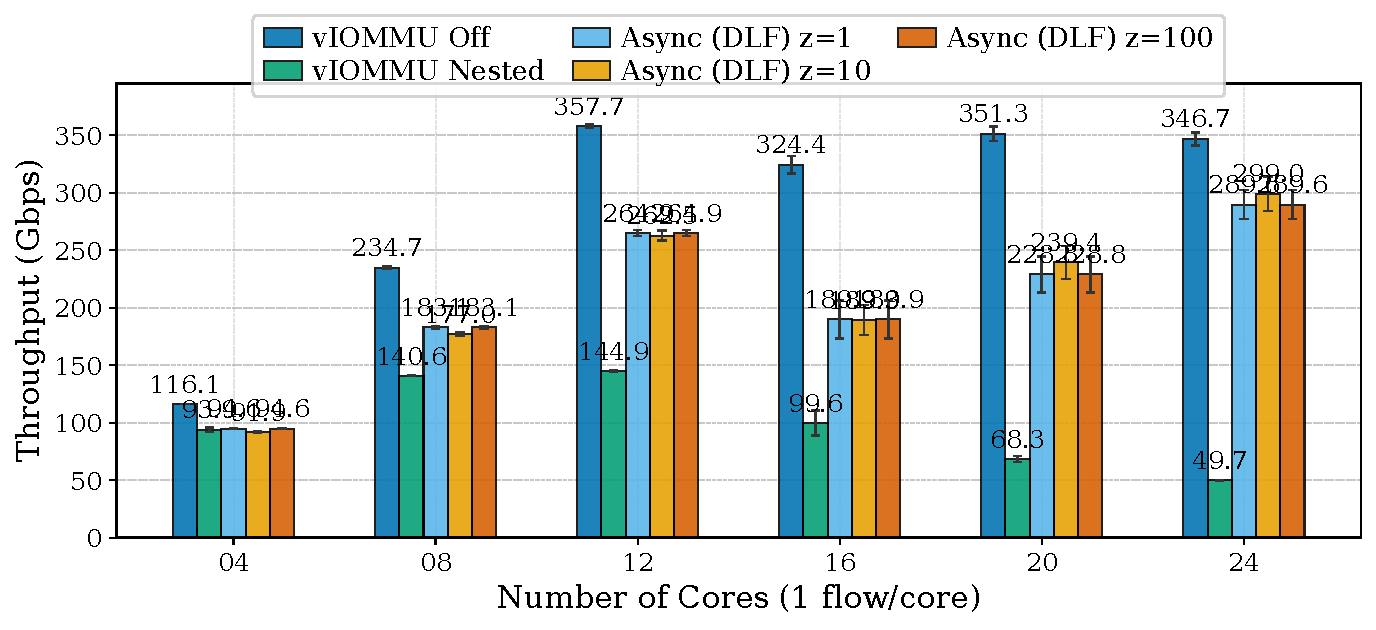
\includegraphics[width=\textwidth]{figures/eval_sensitivity_core_exp-tput.pdf}
%         \Description{Bar chart showing throughput sensitivity analysis when only Async Invalidation is enabled.}
%         \caption{Sensitivity Analysis when only Async Invalidation are enabled }
%         \label{vfree:fig:sensitivity-core}
%     \end{subfigure}
%     \vspace{1em}
%     \begin{subfigure}[b]{\columnwidth}
%         \centering
%         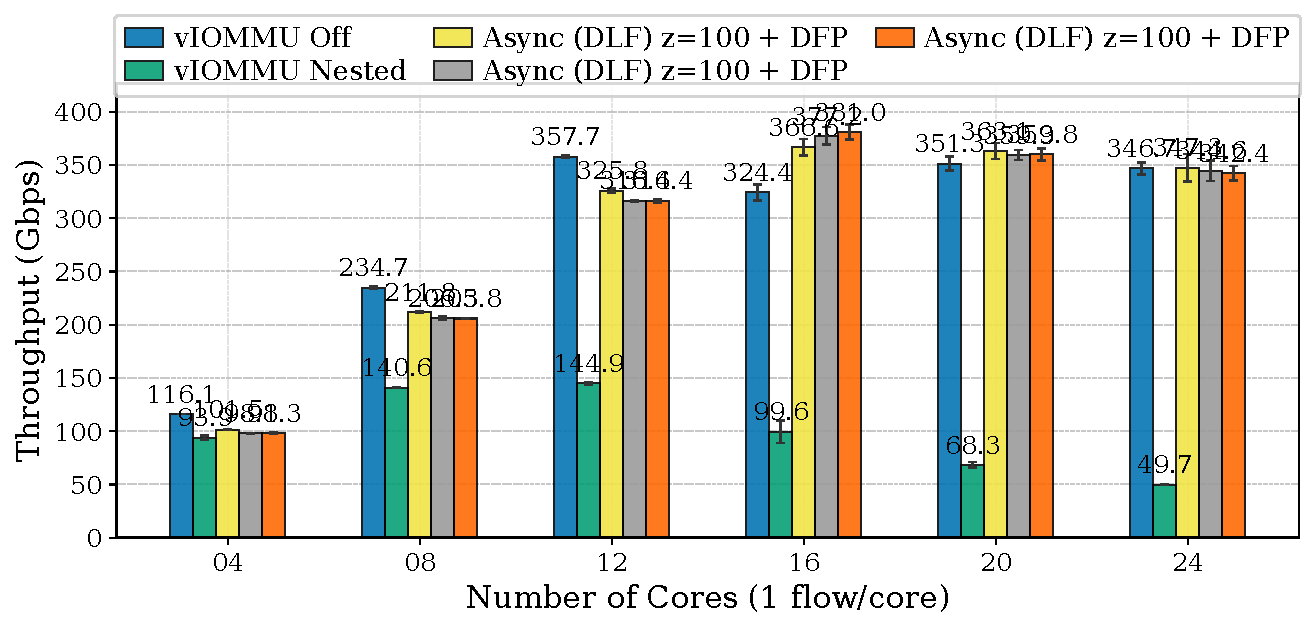
\includegraphics[width=\textwidth]{figures/eval_sensitivity_core_exp_dlf-tput.pdf}
%         \Description{Bar chart showing throughput sensitivity analysis when Async Invalidation is used with DFP.}
%         \caption{Sensitivity Analysis when only Async Invalidation is used in combination with DFP}
%         \label{vfree:fig:sensitivity-dlf}
%     \end{subfigure}
%     \caption{Parameter sensitivity of async invalidation implemented in distributed-leader-follower scheme.
%     Tested on with different maximum flushes per round (z=1, 10, 100)}
%     \label{vfree:fig:sensitivity}
% \end{figure}








\subsubsection{{\vfreename} Scalability with Increasing VM count}
\label{vfree:sec:eval-multi-vm}

Cloud deployments commonly deploy more than one VM per server.
We evaluate how {\vfreename} performance fares with an increasing number of VMs.
We fix the total core budget at 32 (the maximum per socket on our setup) and vary the number of VMs from 1 to 16, dividing the cores equally (\textit{e.g.}, assigning $32/N$ vCPUs) and using a dedicated SR-IOV Virtual Function~\cite{ms_sriov_overview} for each VM.
We report aggregate throughput across all VMs. {We focus on Tx-server setup since it shows the most severe degradation with vIOMMU-on.}


Figure~\ref{vfree:fig:multi-vm} shows that {\vfreename} maintains close-to-vIOMMU-off performance for each evaluated VM count,
while vIOMMU-on results in 80--96\% throughput degradation. As expected, with vIOMMU-on, aggregate throughput {increases} from 16.4\,Gbps with 1~VM to 75.8\,Gbps with 16~VMs.
{This is likely due to each VM independently being able to perform IR-SUB concurrently---increasing the arrival rate of IRs to the IOMMU invalidation queue.}

\begin{figure}[H]
    \centering
    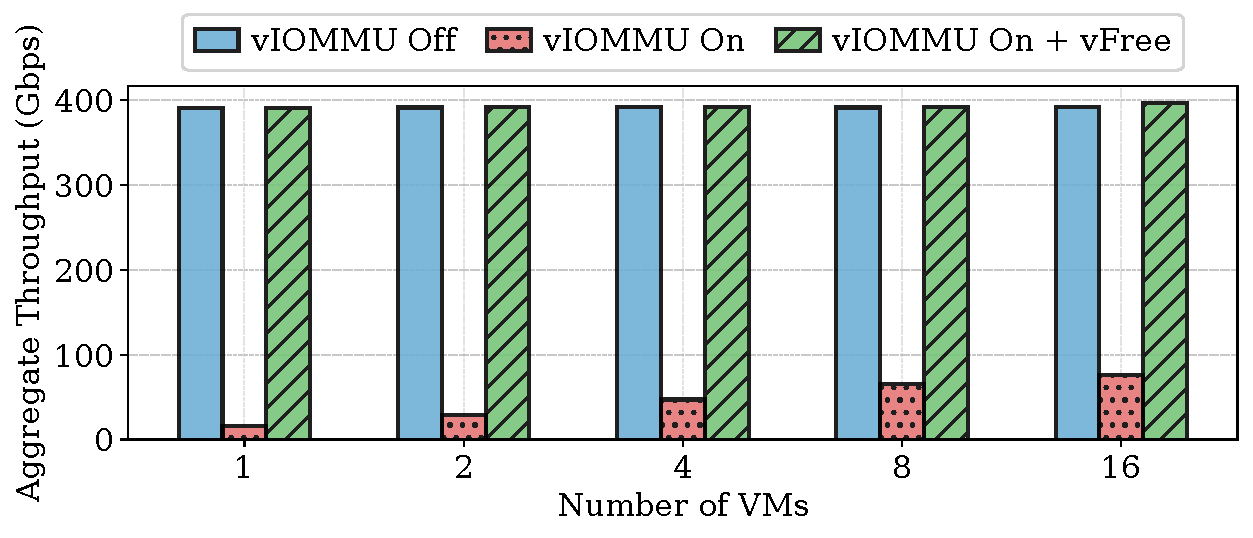
\includegraphics[width=0.75\columnwidth]{figures/many_vm_throughput.pdf}
    \caption{\small {\bf {\vfreename} maintains its benefits with increasing number of VMs per host. Discussion in \S\ref{vfree:sec:eval-multi-vm}}}
%    \vspace{-0.1in}
    \label{vfree:fig:multi-vm}
\end{figure}

% \saksham{Can we get rid of this-->}This is a direct consequence of the intra-VM contention structure identified in \S\ref{vfree:sec:inefficiencies}:
%     each VM has its own emulated invalidation queue,
%     so fewer cores per VM means less intra-VM serialization on the invalidation path.
% However, even in the best case (16~VMs), vIOMMU-on achieves only 19\% of vIOMMU-off throughput.
% {\vfreename} completely eliminates IOMMU overhead and scales well across multi-VM configurations, delivering $5.2$--$24\times$ improvement over vIOMMU-on.

\subsubsection{No Free Lunch: The Cost of {\vfreename} Benefits}
\label{vfree:ssec:cost}
{\vfreename} benefits come with two costs: it requires a dedicated core, and it requires extra memory due to deferred free page. We believe the former is not fundamental: it should be possible to opportunistically distribute the IR-SUB processing to producer threads (\textit{e.g.}, any lightly-loaded producer can become a consumer, and execute IR-SUB on its local core). Nevertheless, even with one dedicated core, {\vfreename} expands the choices of real-world systems: high performance but with weak (or no) IO memory protection, abysmal performance with \textit{significantly underutilized} cores with strict IO memory protection, or, high performance with one dedicated core with strict IO memory protection. For the extra memory, our evaluation results presented in the Appendix-B suggest that the extra memory requirements are less than $4\%$ across all our evaluated workloads.

% The cost of achieving {\vfreename} benefits is an additional core. 


% Cloud deployments commonly partition physical resources among multiple VMs. We evaluate how \vfreename{} performs as the same 32 cores are divided among an increasing number of VMs---from a single 32-vCPU VM to sixteen 2-vCPU VMs.

% We fix the total core budget at 32 and vary the number of VMs
% (1, 2, 4, 8, 16), assigning $32/N$ vCPUs to each of the $N$ VMs.
% Every VM has its own SR-IOV virtual function and runs under the
% same three configurations as in the single-VM experiments.
% We report the aggregate Tx throughput across all VMs.

% Figure~\ref{vfree:fig:multi-vm} shows that \vfreename{} matches vIOMMU-off
% performance at every VM count.
% In contrast, enabling vIOMMU without \vfreename{} causes
% 80--96\% throughput degradation depending on the VM count.

% With vIOMMU-on, aggregate throughput \emph{increases} from 16.4\,Gbps with 1~VM to 75.8\,Gbps with 16~VMs.
% This is a direct consequence of the per-VM contention structure identified in \S\ref{vfree:sec:inefficiencies}:
% each VM has its own emulated invalidation queue,
% so fewer cores per VM means less intra-VM serialization
% on the invalidation path.
% However, even in the best case (16 VMs),
% vIOMMU-on achieves only 19\% of vIOMMU-off throughput.
% \vfreename{} eliminates this bottleneck entirely,
% delivering up to 24$\times$ throughput improvement over vIOMMU-on (1~VM) and 5.2$\times$ at 16~VMs, where the baseline is least degraded.



% \subsubsection{Impact of Consumer Placement.}
% \todo{@Siyuan Add text}

%


\subsection{Related Work}
\label{vfree:sec:related}
% We discuss key works related to {\vfreename}.
% \vfreebrand is the first work that studies IO memory protection in virtualized environments with nested transaction, on modern server hardware architectures.

\para{Bare-metal IO memory protection.}
There is a large and active body of work on enabling IO memory protection with near-zero overheads for the bare metal case~\cite{ben2007price, Malka2015rIOMMU, malka2015efficient, peleg2015utilizing, Markuze2016true, markuze2018damn, RajapakshaIOMMU, Rubin2024FastSafe}. There is also work on rearchitecting IOMMU (\textit{e.g.}, replacing page tables with circular tables~\cite{Malka2015rIOMMU}
    and using hardware support for security checks~\cite{RajapakshaIOMMU}). Collectively, these works have led to mechanisms that enable achieving strict IO memory protection with minimal overheads. 

{\vfreename} builds upon these works for the bare metal case. For example, persistent
mapping for receive buffers has been adopted by Linux (Rx datapath optimizations in \S\ref{vfree:sec:background-datapath}); similarly, as discussed in \S\ref{vfree:sec:impl}, we use the techniques developed in~\cite{Rubin2024FastSafe}. As shown in Figure~\ref{vfree:fig:ablation}, these mechanisms are helpful but not sufficient in virtualized environments---the key focus of our work. Indeed, we show in \S\ref{vfree:sec:inefficiencies} that the performance bottlenecks are quite different in virtualized environments and in fact may require design choices that make very different tradeoffs (\textit{e.g.}, {\vfreename} reduces the number of VM exits by increasing the address translation cost).
    
% % Prior work studies the overhead of IOMMU protection in bare-mental environments.
% Markuze et al.\ proposed shadow DMA buffers that restrict devices to
% permanently mapped memory regions, eliminating IOTLB invalidations and
% achieving up to 5$\times$ higher throughput than strict mode~\cite{Markuze2016true}.  
% DAMN specializes this approach for networking by allocating packet buffers from a
% permanently mapped pool~\cite{markuze2018damn}. Persistent
% mapping for receive buffers has been adopted by Linux (Rx datapath optimizations in \S\ref{vfree:sec:background-datapath}).
% % subsystem, so the copy-based approach cannot support zero-copy workloads.
% % and DAMN is inapplicable to non-networking devices such as NVMe.  
% In fact, the CPU and memory bandwidth cost of copying scales with IO throughput, 
%     limiting the approach at higher link speeds.
% F\&S exploits IO PWCs to reduce the cost of IOTLB misses, 
%     achieving strict safety with near-zero overhead on bare metal~\cite{Rubin2024FastSafe}. 
% F\&S's IOVA allocation strategy and page pools apply to virtualized environments, 
%     but are insufficient:
%     under nested translation, the dominant overhead shifts from the cost of IOTLB misses 
%     to VM exits. \vfreebrand builds on the bare-metal foundations and reduces VM exits due to 
%     cache invalidations, the dominant bottleneck as link speeds increase.

% \vfreebrand requires no IOMMU hardware modification and is 
%     complementary to research that proposes to rearchitect
%     IOMMU (e.g., replacing page tables with circular tables~\cite{Malka2015rIOMMU}
%     and hardware support for security checks~\cite{RajapakshaIOMMU}).
% Faster IOMMU hardware would further amplify gains of \vfreebrand.
% Several proposals rearchitect IOMMU hardware to reduce translation or
% invalidation costs.  Malka et al.\ (rIOMMU) replace the page-table hierarchy
% with a flat circular table for ring-buffer devices~\cite{Malka2015rIOMMU}.  
% Rajapaksha et al.\ proposed a hardware indicator-bit to close the exploitable stale-entry window created by deferred invalidation~\cite{RajapakshaIOMMU}.  
% These approaches are complementary to \vfreebrand: reducing the hardware 
% cost of each invalidation could further amplify the gains from \vfreebrand's software-side batching and serialization elimination.

\para{vIOMMU emulation.}
Amit et al.\ presented an vIOMMU emulation for
    unmodified guests~\cite{Amit2011vIOMMU}. Prior work also optimized other virtualization overhead including 
    memory pinning~\cite{Tian2020coIOMMU} and interrupts~\cite{Gordon2012eli, Har2013paraIO}. All the above work was conducted at 10--100\,Gbps. \vfreebrand extends these works in two ways. First, it presents new insights related to performance bottleneck at 400\,Gbps (\S\ref{vfree:sec:inefficiencies}); and second, {\vfreename} addresses these bottlenecks with software techniques that require no paravirtualization or hardware modifications.

%     with 
%     two optimizations: sidecore offloading and optimistic teardown. 
% Sidecore offloading requires hypervisor modifications and a dedicated core; 
% \vfreebrand uses a push-based design where vCPUs enqueue invalidations into per-CPU buffers without waiting
% or dedicating a core. Optimistic teardown recovers line rate at 10\,GbE,
%     but weakens security guarantees; \vfreebrand preserves strict safety.

\if 0 % this conference is way too weird
LA-vIOMMU added a fixed IOTLB for long-lived mappings and a guest-side DMA mapping cache 
    to reduce VM-exit frequency~\cite{Lv2022LAvIOMMU}.
LA-vIOMMU's guest-side cache optimization targets the map/unmap exit cost; 
    under nested translation, mapping overhead is already low. 
LA-vIOMMU also requires hardware modifications to the IOTLB.
\fi 


% coIOMMU introduced cooperative DMA buffer tracking between
%guest and hypervisor for fine-grained memory pinning~\cite{Tian2020coIOMMU}. 
% coIOMMU targets the memory pinning problem --- determining which guest pages to pin in host memory---which 
% is orthogonal to the IOTLB invalidation serialization that \vfreebrand addresses.  

% Parallel efforts have targeted other virtualization overheads.  Gordon et al.\
% (ELI) and Har'El et al.\ reduced interrupt and exit costs for assigned
% devices, recovering near-native throughput~\cite{Gordon2012eli, Har2013paraIO}.  
% These optimizations are complementary to \vfreebrand, which focuses on the IOMMU emulation path rather than the interrupt delivery path.




\para{virtIO IOMMU.} \vfreebrand targets hardware-assisted vIOMMU, not virtio-IOMMU;
    despite that, the {\vfreename} ideas may apply.
vIOMMU offers VMs with native hardware interfaces, 
    ensuring compatibility with nested translation and modern drivers.
It is supported by mainstream systems such as QEMU~\cite{qemu_10_0}.
On our platform (\S\ref{vfree:sec:inefficiencies}),
    virtio-IOMMU can only hit 51\% of the vanilla 
    vIOMMU throughput with nested translation.
%    , and just 9\% compared to vIOMMU Off and \vfreename{}.}

% \tianyin{@Siyuan: do we have one result that virtio-IOMMU is slower?}



% Besides hardware-assisted vIOMMU, IOMMU can be virtualized through virtio-IOMMU, a paravirtualization method 
%    that requires a synchronized software stack involving both a guest-side frontend driver and a host-side backend.
% Each DMA operation requires a hypercall, mutex acquisition, and software tree traversal.
% \schaic{I replaced VM exit with hypercall to reinforce their VM exit nature. @Owen Is it one hypercall on both map and unmap time? If so, we should explicitly state it. Also, let's explain from functionality wise what is the hypercall doing.}
% Although this implementation is simple, it is considerably less efficient compared to Intel VT-d,
% which does not require a VM exit when new mappings are built.
% \schaic{@Owen, let's include a percentage number based on our profiling. aka vanilla virtio vs. vanilla nested strict.}

% The virtio-vIOMMU also introduces a non-architectural software abstraction that precludes the use of unmodified guest vendor drivers.
% These high-performance proprietary stacks and userspace drivers (e.g., DPDK) often bypass standard kernel DMA APIs to interact directly with architectural register sets.
% Because virtio-IOMMU exposes a generic software device rather than the expected hardware interfaces, 
%    these drivers may fail to detect a compatible IOMMU, breaking support for advanced features like p2p DMA and PASID.
% \schaic{@Owen, can you help search for reference to support our argmument.s}
    
% Building upon the vIOMMU framework, our work provides virtual machines with the exact same architectural interface used by a bare-metal kernel. 
% It ensures compatibility with emerging hardware-assisted nested translation and modern drivers.
% Our approach targets the production-standard interface used in modern data centers:
%    \vfreebrand eliminates vIOMMU overhead while maintaining strict safety protection.  
    % allowing for optimizations in DMA mapping and IOTLB invalidation that remain entirely transparent to the guest while utilizing hardware-assisted nested translation.

\subsection{Concluding Remarks}

We show that it is feasible to achieve both strict IO memory protection
    and high-performance DMA by 
    carefully analyzing performance bottlenecks
    and reconstructing the software stack.
{\vfreename} makes a practical solution which can be readily applied to 
    commodity OSes and hypervisors.
We hope our work to greatly improve the safety 
    and security of real-world systems with emerging high-speed 
    devices.
% \begin{figure}[t]
%     \centering
%     \begin{subfigure}[b]{0.32\textwidth}
%         \centering
%         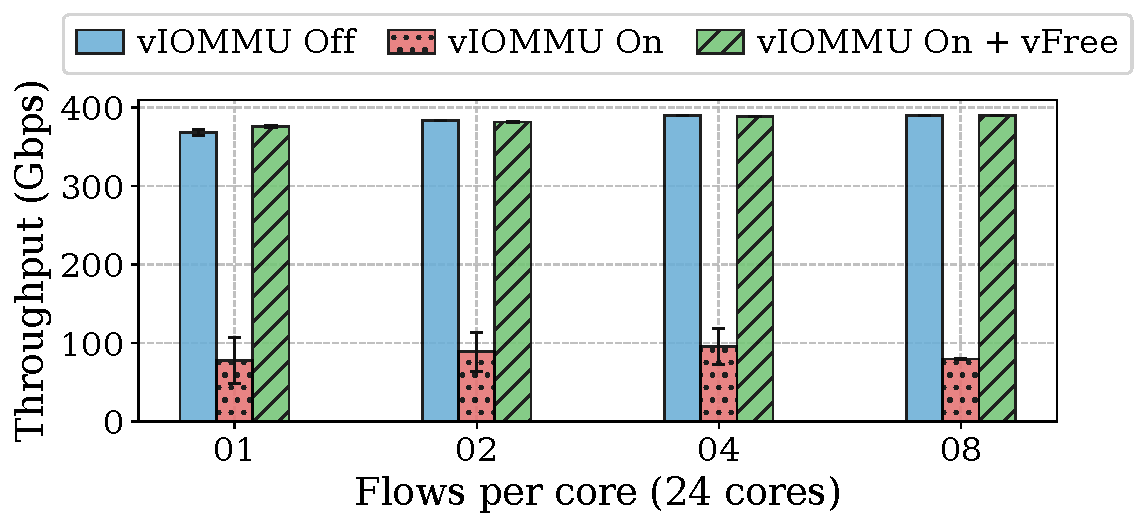
\includegraphics[width=\textwidth]{figures/stress_exp-tput.pdf}
%         \caption{Throughput}
%         \label{vfree:fig:stress-tput}
%     \end{subfigure}
%     \hfill
%     \begin{subfigure}[b]{0.32\textwidth}
%         \centering
%         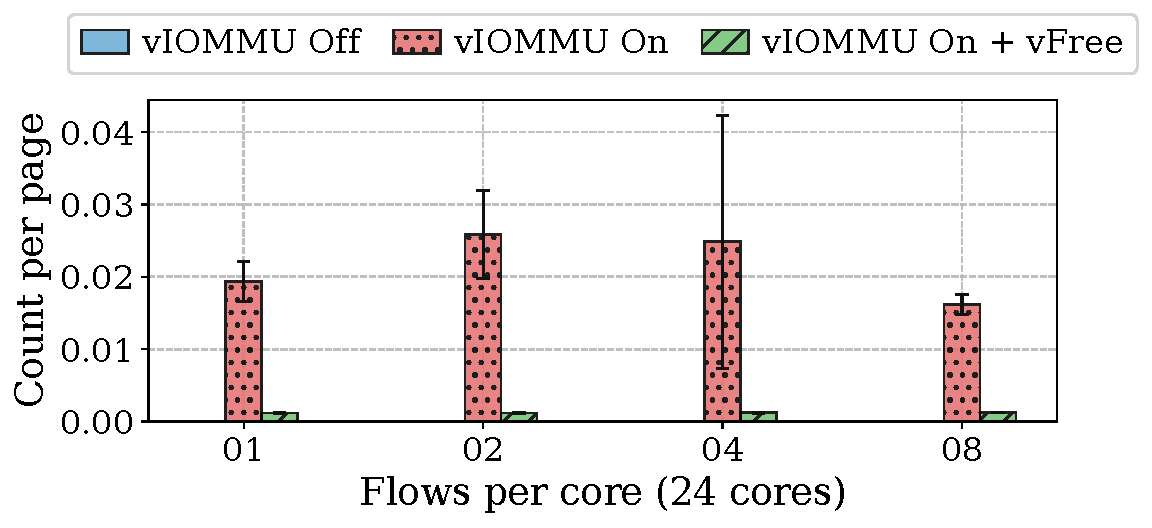
\includegraphics[width=\textwidth]{figures/stress_exp-qi_submit_sync-count_per_page.pdf}
%         \caption{IR-SUB count per page}
%         \label{vfree:fig:stress-qi}
%     \end{subfigure}
%     % \begin{subfigure}[b]{0.32\textwidth}
%     %     \centering
%     %     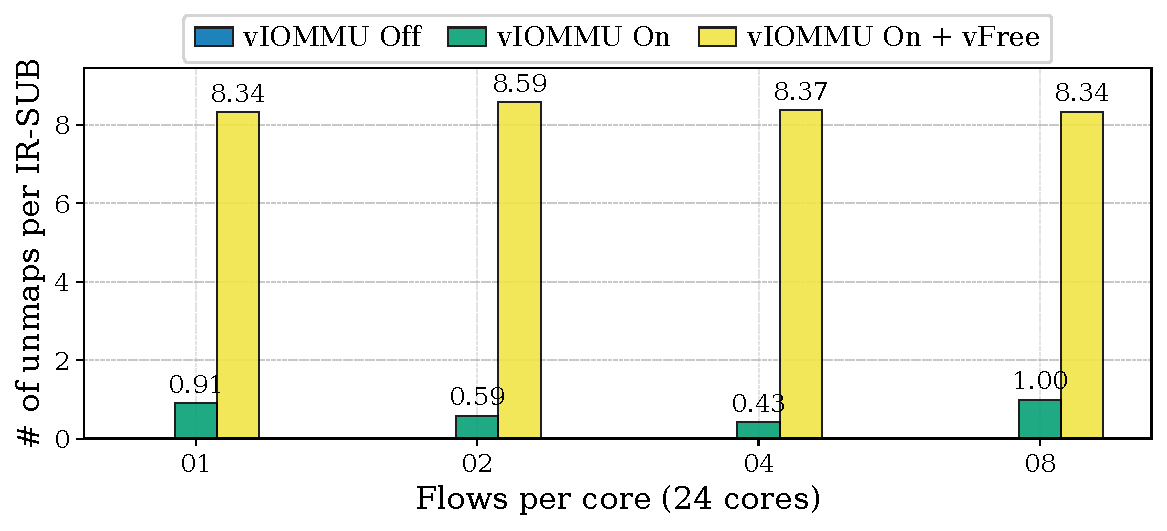
\includegraphics[width=\textwidth]{figures/stress_exp-unmap_to_qi_submit_ratio.pdf}
%     %     \caption{Number of unmap calls per IR-SUB}
%     %     \label{vfree:fig:stress-qi}
%     % \end{subfigure}
%     \hfill
%     \begin{subfigure}[b]{0.32\textwidth}
%         \centering
%         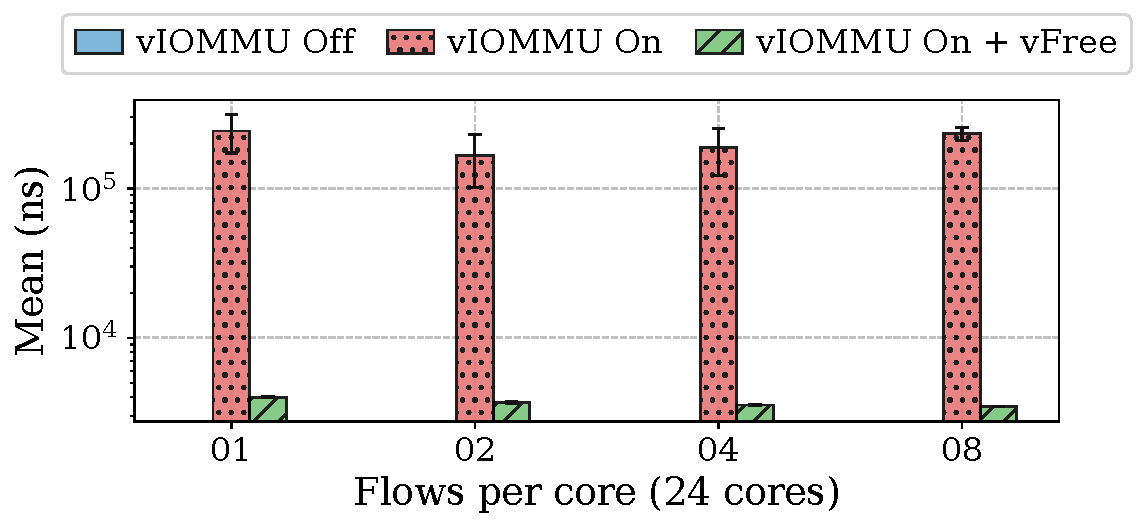
\includegraphics[width=\textwidth]{figures/stress_exp-cache_tag_flush_range-mean_ns.pdf}
%         \caption{IOTLB invalidation overhead per unmap}
%         \label{vfree:fig:stress-flush}
%     \end{subfigure} 
%     \caption{Rx stress test (multiple flows per core): \vfreename{} consistently matches vIOMMU-off throughput.
%     }
%     \label{vfree:fig:stress}
% \end{figure}

% \begin{figure}[t]
%     \centering
%     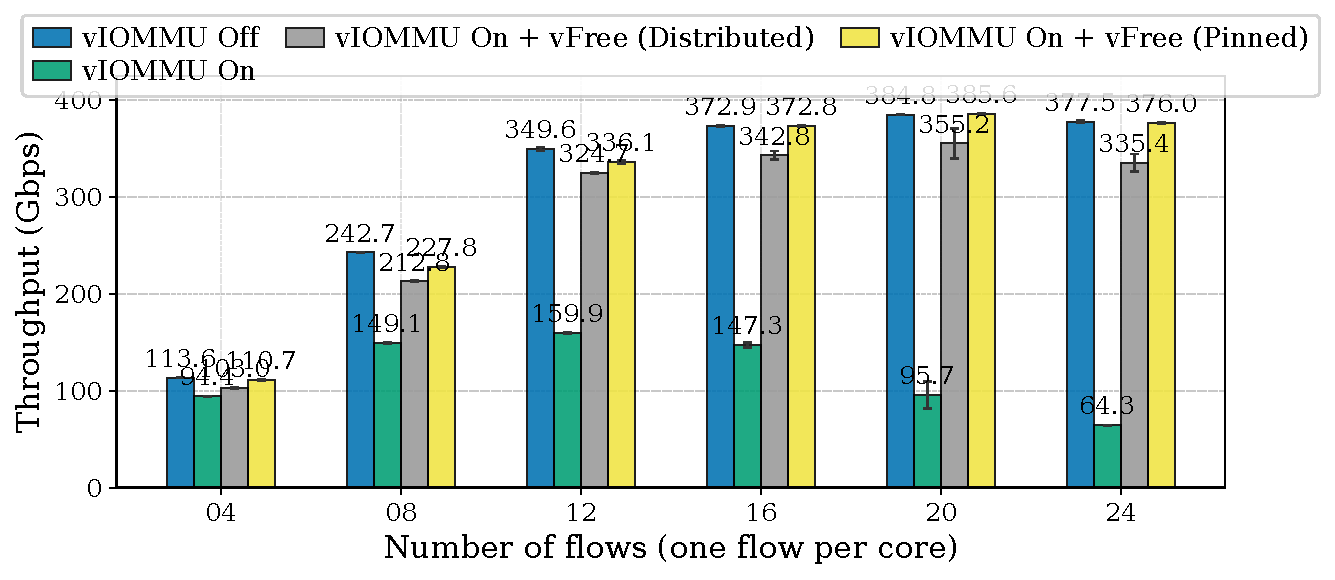
\includegraphics[width=\columnwidth]{figures/eval_core_exp_dlf-tput.pdf}
%     \caption{Rx throughput with DLF.\todo{Rerun with DLF (we should hit 400Gbps)}}
%     \label{vfree:fig:eval-core-dlf}
% \end{figure}

% \begin{figure}[t]
%     \centering
%     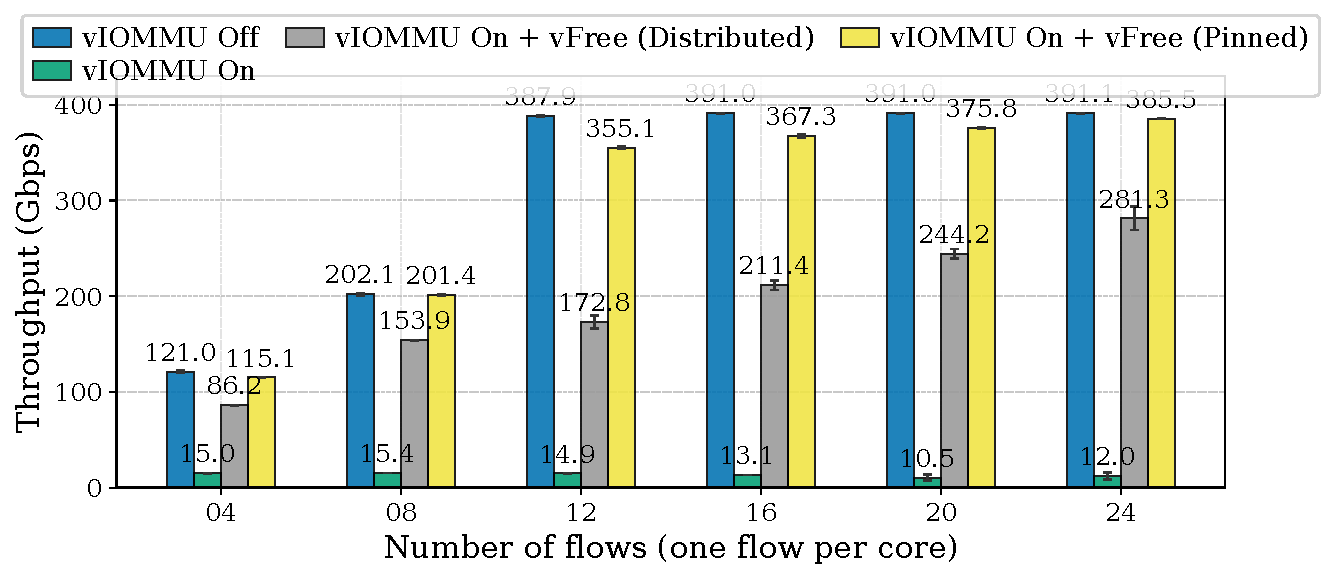
\includegraphics[width=\columnwidth]{figures/tx-ebpf-dlf-tput.pdf}
%     \caption{Tx throughput with DLF.\todo{This is the best we have now}}
%     \label{vfree:fig:tx-dlf}
% \end{figure}

\subsection{Appendix}
\subsubsection{Threat Model}
\label{vfree:sec:threat_model}

Modern OSes typically offer two modes of IO memory protection. 
The strongest guarantee is that of so-called strict mode~\cite{nadav2010iommu, Amit2011vIOMMU} 
% \vfreebrand maintains strict IO memory protection provided by 
    % Linux's strict mode~\cite{} 
    which enforces  
    the free-after-invalidation invariant to ensure % I assume it's the invariant was made early in the design
    \emph{no page can be freed with a stale entry 
        that permits access to the page in hardware caches (\textit{e.g.}, IOTLB)}.
This invariant is key to data integrity~\cite{AlexCodeInjection} and confidentiality~\cite{RajapakshaIOMMU}.
The other mode---referred to as the lazy or deferred mode~\cite{RajapakshaIOMMU,AlexCodeInjection}---provides 
    weaker protection because it violates this invariant by
    deferring invalidation after the DMA 
    buffer is unmapped, creating a window of vulnerabilities to integrity and confidentiality attacks.

{\vfreename} follows the threat model of strict protection mode of Linux IOMMU~\cite{nadav2010iommu} and prior work~\cite{markuze2018damn,Amit2011vIOMMU,RajapakshaIOMMU}.
Our trusted computing base includes the guest OS (including the device driver), 
    the host OS, hypervisor (including the vIOMMU subsystem), 
    and the underlying hardware (CPU, memory system, and physical IOMMU).
We assume that the guest OS correctly configures and manages DMA mappings
    and that the host OS and physical IOMMU faithfully enforces these mappings.
{\vfreename} defends against attacks that control malicious or compromised IO devices.
The focus is protection from unauthorized DMAs in the intra-VM context.

    % which attempt to 
    % access memory beyond regions assigned by the guest OS
    % or reuse stale IOVAs after mappings were revoked.

Boot-time DMA attacks are assumed to be mitigated independently and 
    thus out of the scope of IOMMU protection~\cite{markuze2018damn}.
Data integrity attacks performed while the device \emph{legitimately} 
    holds a mapping (\textit{e.g.}, a malicious NIC modifying packet payload before the DMA is complete) 
    is equivalent to corruption on disk or a man-in-the-middle attack; 
    this is also outside the IOMMU's scope of protection.
% For sub-page vulnerabilities~\cite{}, we provide the same defense 
%    as Linux's strict mode;
% \leshna{needs slight rephrasing, it reads like we claim linux strict doesn't handle it, we want to state we don't change how it is handles so we don't introduce any attack here}
%    \vfreebrand neither introduces nor mitigates this class.

\subsubsection{Memory Overhead of \vfreename}

% \textbf{Parameter sensitivity of async invalidation.}

% Figure \ref{vfree:fig:sensitivity} shows the parameter sensitivity of async invalidation implemented in distributed-leader-follower scheme.
% We test with different maximum flushes per round (z=1, 10, 100).
% Regardless of whether DFP is enabled, \vfreebrand's performance is not sensitive to the number of maximum flushes per round.

Using deferred protection in {\vfreename} provides higher performance at the cost of potentially larger memory utilization. This is because we delay the time when a page is freed. Therefore, for achieving any given throughput, using deferred free page would result in larger number of {\em active pages} at any point of time, where a page is considered active from the moment it is mapped to an IOVA, until it is freed. 

% A trade-off made by \vfreename{} is to 
%     defer the free page operation \emph{after} invalidation.
%This may require more active physical pages to be allocated by the driver 
%    to reach the same throughput, compared with vIOMMU off. 
% Intuitively, to achieve the same throughput, more pages will be activated by {\vfreename}. 
We show that the memory overhead of \vfreebrand
for our evaluation setup is pretty small.
We run 24 Iperf flows for 120 seconds, sampling the number of active pages every 0.5 seconds for {\vfreename} and vIOMMU-off.
\vfreename's throughput is within 1\% of vIOMMU-off in these experiments.

\begin{figure}[!htbp]
    \centering
    \begin{subfigure}[b]{0.49\columnwidth}
        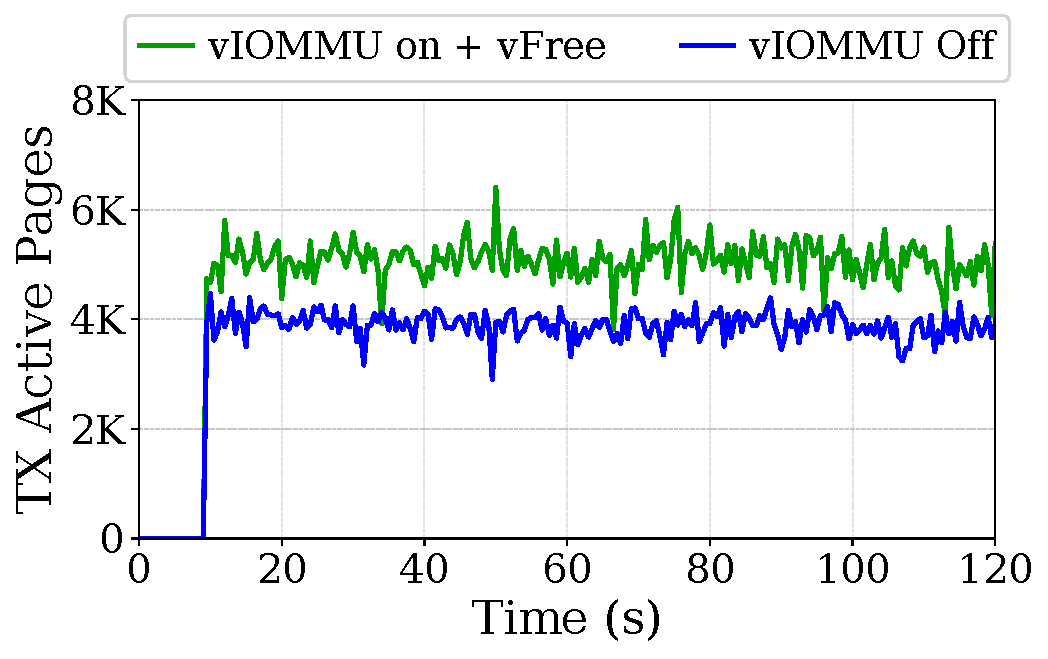
\includegraphics[width=\columnwidth]{figures/tx_mem/mem_fig_tx_active_pages.pdf}
        \Description{Plot showing TX page usage over time.}
        \caption{Active pages required by the Tx datapath over time.}
        \label{vfree:fig:tx_exp_memory_tx}
    \end{subfigure}
    \begin{subfigure}[b]{0.49\columnwidth}
        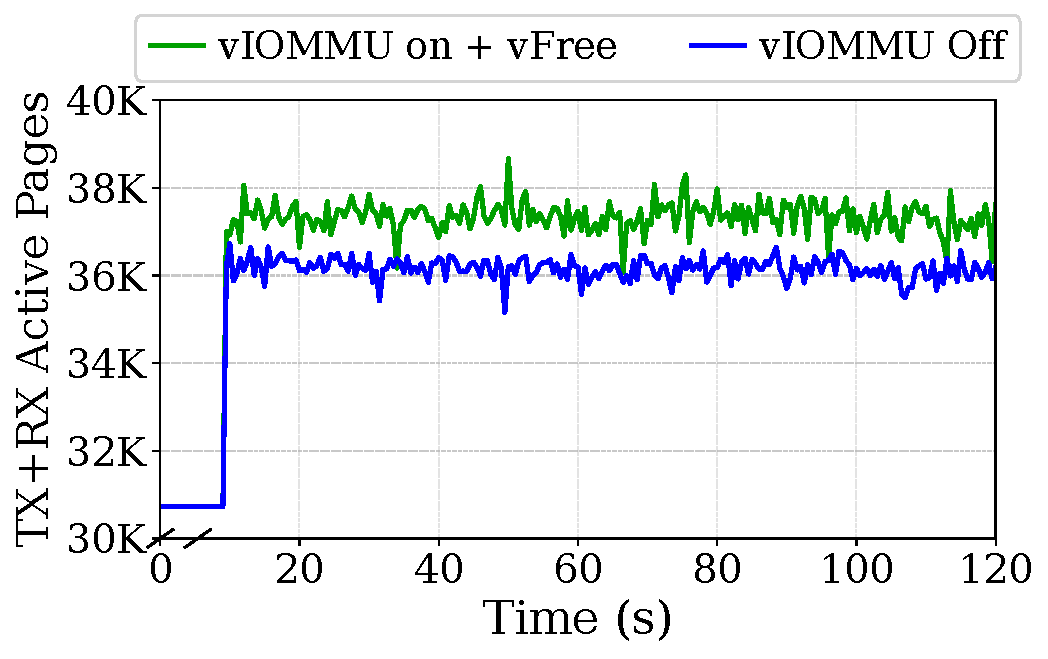
\includegraphics[width=\columnwidth]{figures/tx_mem/mem_fig_tx_rx_active_pages.pdf}
        \Description{Plot showing RX+TX page usage over time.}
        \caption{Active pages required by the Rx and Tx datapath over time.}
        \label{vfree:fig:tx_exp_memory_total}
    \end{subfigure}
    \caption{For Tx-server setup, {\vfreename} incurs less than 3.3\%
     memory overhead over vIOMMU-off.}
    \label{vfree:fig:tx_memory}
\end{figure}

\begin{figure}[!htbp]
    \centering
    \begin{subfigure}[b]{0.49\columnwidth}
        
\includegraphics[width=\columnwidth]{figures/rx_mem/mem_fig_tx_active_pages.pdf}
        \Description{Plot showing TX page usage over time.}
        \caption{Active pages required by the Tx datapath over time.}
        \label{vfree:fig:rx_exp_memory_tx}
    \end{subfigure}
    \begin{subfigure}[b]{0.49\columnwidth}
        
\includegraphics[width=\columnwidth]{figures/rx_mem/mem_fig_tx_rx_active_pages.pdf}
        \Description{Plot showing RX+TX page usage over time.}
        \caption{Active pages required by the Rx and Tx datapath over time.}
        \label{vfree:fig:rx_exp_memory_total}
    \end{subfigure}
    \caption{For Rx-server setup, {\vfreename} incurs less than 2.3\% additional memory overhead over vIOMMU-off.}
    \label{vfree:fig:rx_memory}
\end{figure}

\para{Tx-server.} We measure active physical pages for Tx held by the mlx5 driver. The Tx datapath shows an increase by 30.5\%, an inherent cost of deferring free page (Figure~\ref{vfree:fig:tx_exp_memory_tx}).
However, Figure~\ref{vfree:fig:tx_exp_memory_total} shows that when accounting for both Tx and Rx-datapath active pages, the total page count increases by only 3.28\% over vIOMMU-off,
because the page pool on the Rx side retains pages in its cache rather than actively releasing them to the kernel allocator.

\para{Rx-server.} 
% We measure active page count for Rx using page pool stats~\cite{linux_page_pool,linux_page_pool_stats}.
As shown in Figure~\ref{vfree:fig:rx_exp_memory_total}
\vfreename{} requires only 2.23\% more total pages over vIOMMU-off.
The active page count for Tx datapath only (Figure~\ref{vfree:fig:rx_exp_memory_tx}) shows a larger relative difference,
but memory consumption is dominated by the Rx datapath, so the overall memory overhead is minimal.


\tagpdfsetup{para/tagging=true}
